
% This LaTeX was auto-generated from MATLAB code.
% To make changes, update the MATLAB code and republish this document.

\documentclass{article}
\usepackage{graphicx}
\usepackage{color}

\sloppy
\definecolor{lightgray}{gray}{0.5}
\setlength{\parindent}{0pt}

\begin{document}

    
    
\subsection*{Contents}

\begin{itemize}
\setlength{\itemsep}{-1ex}
   \item Guaranteed Automatic Integration Library (GAIL) Version 2.2 Documentation
   \item Introduction
   \item Functions
   \item Demos
   \item Website
   \item GAIL License
   \item Developed by
   \item Downloads
   \item Requirements
   \item Documentation
   \item General Usage Notes
   \item Installation Instruction
   \item Tests
   \item Contact Information
   \item Acknowledgements
   \item 1-D approximation
   \item 1-D integration
   \item 1-D minimization
   \item Higher dimensional integration
   \item GAIL Demos
   \item 1-D approximation
   \item 1-D minimization
   \item 1-D integration
   \item Higher dimensional integration
   \item funappx\_g
   \item Syntax
   \item Description
   \item Guarantee
   \item Examples
   \item See Also
   \item References
   \item funmin\_g
   \item Syntax
   \item Description
   \item Guarantee
   \item Examples
   \item See Also
   \item References
   \item integral\_g
   \item Syntax
   \item Description
   \item Guarantee
   \item Examples
   \item See Also
   \item References
   \item meanMC\_g
   \item Syntax
   \item Description
   \item Guarantee
   \item Examples
   \item See Also
   \item References
   \item cubMC\_g
   \item Syntax
   \item Description
   \item Guarantee
   \item Examples
   \item See Also
   \item References
   \item cubLattice\_g
   \item Syntax
   \item Description
   \item Guarantee
   \item Examples
   \item See Also
   \item References
   \item cubSobol\_g
   \item Syntax
   \item Description
   \item Guarantee
   \item Examples
   \item See Also
   \item References
   \item Demos for funappx\_g
   \item Approximate a highly fluctuating curve using \textbf{funappx\_g}.
   \item Function definition
   \item Function approximation
   \item Plots of the function and approximant
   \item Plot of the apprroximation errors
   \item A slightly different example
   \item A workaround
   \item A better way
   \item References
   \item A GUI (graphical user interface) for \textbf{funappx\_g}
   \item Function definition
   \item Function Approximation
   \item Process to Generate Grid Points
   \item References
   \item Demos for funmin\_g
   \item Function definition
   \item Function minimization
   \item Plots of the function and its minimum
   \item A fix
   \item References
   \item Compare \textbf{funmin\_g} with \textbf{fminbnd}
   \item Function definition
   \item Function minimization
   \item Plot of the function and minima
   \item References
   \item Demos for integral\_g
   \item Integrate a spiky function using \textbf{integral\_g}
   \item Function definition
   \item Plot of the spiky function
   \item Integral approximation
   \item Compute apprroximation errors
   \item References
   \item Demos for meanMC\_g
   \item Demos for cubMC\_g
   \item Basic integration parameters set up
   \item First test: $\Sigma=I_d$ (Monte Carlo cubMC\_g)
   \item Second test: $\Sigma=0.4I_d + 0.6\bf{1}\bf{1}^T$ (Monte Carlo cubMC\_g)
   \item Third test: $\Sigma=0.4I_d + 0.6\bf{1}\bf{1}^T$ (Monte Carlo cubMC\_g)
   \item APPENDIX: Auxiliary function definitions
   \item References
   \item Estimation of normal probabilities by \textbf{cubSobol\_g}
   \item Basic integration parameters set up
   \item First test: $\Sigma=I_d$ (quasi-Monte Carlo cubSobol\_g)
   \item Second test: $\Sigma=0.4I_d + 0.6\bf{1}\bf{1}^T$ (quasi-Monte Carlo cubSobol\_g)
   \item Third test: $\Sigma=0.4I_d + 0.6\bf{1}\bf{1}^T$ (quasi-Monte Carlo cubSobol\_g)
   \item Third test with IID Monte Carlo (Monte Carlo meanMC\_g)
   \item APPENDIX: Auxiliary function definitions
   \item References
   \item The following output was obtained on 2014-10-13  by Lan Jiang
\end{itemize}
\begin{verbatim}
function gail_ug_2()
\end{verbatim}


\subsection*{Guaranteed Automatic Integration Library (GAIL) Version 2.2 Documentation}

\begin{par}
GAIL (Guaranteed Automatic Integration Library) is created, developed, and maintained by Fred Hickernell (Illinois Institute of Technology), Sou-Cheng Choi (NORC at the University of Chicago and IIT), Yuhan Ding (IIT), Lan Jiang (IIT), Lluis Antoni Jimenez Rugama (IIT), Xin Tong (University of Illinois at Chicago), Yizhi Zhang (IIT), and Xuan Zhou (IIT).
\end{par} \vspace{1em}
\begin{par}
GAIL is a suite of algorithms for integration problems in one, many, and infinite dimensions, and whose answers are guaranteed to be correct.
\end{par} \vspace{1em}


\subsection*{Introduction}

\begin{par}

\end{par} \vspace{1em}


\subsection*{Functions}

\begin{par}

\end{par} \vspace{1em}


\subsection*{Demos}

\begin{par}

\end{par} \vspace{1em}


\subsection*{Website}

\begin{par}
For more information about GAIL, visit \begin{verbatim}Gailteam\end{verbatim}
\end{par} \vspace{1em}


\subsection*{GAIL License}

\begin{verbatim}
%Copyright � 2015, Illinois Institute of Technology. All rights reserved.
%
% Redistribution and use in source and binary forms, with or without
% modification, are permitted provided that the following conditions are
% met:
%
%   * Redistributions of source code must retain the above copyright
%     notice, this list of conditions and the following disclaimer.
%
%   * Redistributions in binary form must reproduce the above copyright
%     notice, this list of conditions and the following disclaimer in the
%     documentation and/or other materials provided with the distribution.
%
%   * Neither the name of Illinois Institute of Technology nor the names of
%     its contributors may be used to endorse or promote products derived
%     from this software without specific prior written permission.
%
% THIS SOFTWARE IS PROVIDED BY THE COPYRIGHT HOLDER AND CONTRIBUTORS
% "AS IS" AND WITHOUT ANY WARRANTY OF ANY KIND, WHETHER EXPRESS, IMPLIED,
% STATUTORY OR OTHERWISE, INCLUDING WITHOUT LIMITATION WARRANTIES OF
% MERCHANTABILITY, FITNESS FOR A PARTICULAR USE AND NON-INFRINGEMENT, ALL
% OF WHICH ARE HEREBY EXPRESSLY DISCLAIMED. MOREOVER, THE USER OF THE
% SOFTWARE UNDERSTANDS AND AGREES THAT THE SOFTWARE MAY CONTAIN BUGS,
% DEFECTS, ERRORS AND OTHER PROBLEMS THAT COULD CAUSE SYSTEM FAILURES, AND
% ANY USE OF THE SOFTWARE SHALL BE AT USER?S OWN RISK. THE COPYRIGHT
% HOLDERS AND CONTRIBUTORS MAKES NO REPRESENTATION THAT THEY WILL ISSUE
% UPDATES OR ENHANCEMENTS TO THE SOFTWARE.
%
% IN NO EVENT WILL THE COPYRIGHT HOLDER OR CONTRIBUTORS BE LIABLE FOR ANY
% DIRECT, INDIRECT, SPECIAL, INCIDENTAL, CONSEQUENTIAL, EXEMPLARY OR
% PUNITIVE DAMAGES, INCLUDING, BUT NOT LIMITED TO, DAMAGES FOR INTERRUPTION
% OF USE OR FOR LOSS OR INACCURACY OR CORRUPTION OF DATA, LOST PROFITS, OR
% COSTS OF PROCUREMENT OF SUBSTITUTE GOODS OR SERVICES, HOWEVER CAUSED
% (INCLUDING BUT NOT LIMITED TO USE, MISUSE, INABILITY TO USE, OR
% INTERRUPTED USE) AND UNDER ANY THEORY OF LIABILITY, INCLUDING BUT NOT
% LIMITED TO CONTRACT, STRICT LIABILITY, OR TORT (INCLUDING NEGLIGENCE OR
% OTHERWISE) ARISING IN ANY WAY OUT OF THE USE OF THIS SOFTWARE, EVEN IF
% ADVISED OF THE POSSIBILITY OF SUCH DAMAGE AND WHETHER OR NOT THE
% COPYRIGHT HOLDER AND CONTRIBUTORS WAS OR SHOULD HAVE BEEN AWARE OR
% ADVISED OF THE POSSIBILITY OF SUCH DAMAGE OR FOR ANY CLAIM ALLEGING
% INJURY RESULTING FROM ERRORS, OMISSIONS, OR OTHER INACCURACIES IN THE
% SOFTWARE OR DESTRUCTIVE PROPERTIES OF THE SOFTWARE.  TO THE EXTENT THAT
% THE LAWS OF ANY JURISDICTIONS DO NOT ALLOW THE FOREGOING EXCLUSIONS AND
% LIMITATION, THE USER OF THE SOFTWARE AGREES THAT DAMAGES MAY BE
% DIFFICULT, IF NOT IMPOSSIBLE TO CALCULATE, AND AS A RESULT, SAID USER HAS
% AGREED THAT THE MAXIMUM LIABILITY OF THE COPYRITGHT HOLDER AND
% CONTRIBUTORS SHALL NOT EXCEED US$100.00.
%
% THE USER OF THE SOFTWARE ACKNOWLEDGES THAT THE SOFTWARE IS BEING PROVIDED
% WITHOUT CHARGE, AND AS A RESULT, THE USER, ACKNOWLEDGING THAT HE OR SHE
% HAS READ THE SAME, AGREES THAT THE FOREGOING LIMITATIONS AND RESTRICTIONS
% REPRESENT A REASONABLE ALLOCATION OF RISK.%% Guaranteed Automatic Integration Library (GAIL)
%
% GAIL Version 2.2, 2017.
% See LICENSE.m for copyright and disclaimer.
%
% GAIL is a suite of algorithms for integration problems in one and many
% dimensions, and whose answers are guaranteed to be correct.
%
%
%
\end{verbatim}


\subsection*{Developed by}

\begin{par}
Fred Hickernell, Sou-Cheng Choi, and their collaborators including Yuhan Ding, Lan Jiang, Lluis Antoni Jimenez Rugama, Yizhi Zhang and Xuan Zhou, Department of Applied Mathematics, Illinois Institute of Technology (IIT) and  Xin Tong, Department of Mathematics, Statistics, and Computer Science, University of Illinois at Chicago. We thank the contributions of Xincheng Sheng, and the IIT class of Math 573 Reliable Mathematical Software, Fall 2013.
\end{par} \vspace{1em}
\begin{par}
Please cite the following software, papers, and materials:
\end{par} \vspace{1em}
\begin{par}
Sou-Cheng T. Choi, "MINRES-QLP Pack and Reliable Reproducible Research via Supportable Scientific Software," Journal of Open Research Software, Volume 2, Number 1, e22, pp. 1-7, 2014. (describes principles of Reliable Reproducible Research and Supportable Scientific Software)
\end{par} \vspace{1em}
\begin{par}
Sou-Cheng T. Choi, Yuhan Ding, Fred J. Hickernell, Lan Jiang, Lluis Antoni Jimenez Rugama, Xin Tong, Yizhi Zhang, and Xuan Zhou, GAIL: Guaranteed Automatic Integration Library (Version 2.2) [MATLAB Software], 2017. Available from \begin{verbatim}http://gailgithub.github.io/GAIL_Dev/\end{verbatim} (this software)
\end{par} \vspace{1em}
\begin{par}
Sou-Cheng T. Choi, Yuhan Ding, Fred J.Hickernell, Xin Tong, "Local Adaption for Approximation and Minimization of Univariate Functions," Journal of Complexity 40, pp. 17-33, 2017. (describes \textbf{funappx\_g.m} and \textbf{funmin\_g.m})
\end{par} \vspace{1em}
\begin{par}
Sou-Cheng T. Choi and Fred J. Hickernell, "IIT MATH-573 Reliable Mathematical Software" [Course Slides], Illinois Institute of Technology, Chicago, IL, 2013. Available from \begin{verbatim}http://gailgithub.github.io/GAIL_Dev/\end{verbatim} (develops practices of Reliable Reproducible Research and Supportable Scientific Software)
\end{par} \vspace{1em}
\begin{par}
Nicholas Clancy, Yuhan Ding, Caleb Hamilton, Fred J. Hickernell, and Yizhi Zhang, "The Cost of Deterministic, Adaptive, Automatic Algorithms: Cones, Not Balls," Journal of Complexity 30, pp. 21-45, 2014. (describes deprecated \textbf{integralPenalty\_g.m} and deprecated \textbf{funappxtau\_g.m})
\end{par} \vspace{1em}
\begin{par}
Yuhan Ding, "Guaranteed Adaptive Univariate Function Approximation," PhD thesis, Illinois Institute of Technology, 2015. (describes deprecated \textbf{funappxPenalty\_g.m})
\end{par} \vspace{1em}
\begin{par}
Fred J. Hickernell, Lan Jiang, Yuewei Liu, and Art B. Owen, "Guaranteed conservative fixed width confidence intervals via Monte Carlo sampling," Monte Carlo and Quasi-Monte Carlo Methods 2012 (J. Dick, F. Y. Kuo, G. W. Peters, and I. H. Sloan, eds.), Springer-Verlag, Berlin, pp. 105-128, 2014. (describes \textbf{meanMC\_g.m} and \textbf{cubMC\_g.m})
\end{par} \vspace{1em}
\begin{par}
Fred J. Hickernell and Lluis Antoni Jimenez Rugama, "Reliable adaptive cubature using digital sequences", Monte Carlo and Quasi-Monte Carlo Methods: MCQMC, Leuven, Belgium, April 2014 (R. Cools and D. Nuyens, eds.), Springer Proceedings in Mathematics and Statistics, vol. 163, Springer-Verlag, Berlin, 2016, arXiv:1410.8615 [math.NA], pp. 367-383. (describes \textbf{cubSobol\_g.m})
\end{par} \vspace{1em}
\begin{par}
Fred J. Hickernell, Lluis Antoni Jimenez Rugama a, and D. Li,"Adaptive quasi-\{M\}onte \{C\}arlo methods, 2017+, submitted for publication, arXiv:1702.01491 [math.NA].
\end{par} \vspace{1em}
\begin{par}
Fred J. Hickernell, Martha Razo, and Sunny Yun, "Reliable Adaptive Numerical Integration", 2015+, working. (describes \textbf{integral\_g.m})
\end{par} \vspace{1em}
\begin{par}
Lan Jiang, Guaranteed Adaptive Monte Carlo Methods for Estimating Means of Random Variables, Ph.D Thesis, Illinois Institute of Technology, 2016. (describes \textbf{meanMC\_g.m} and \textbf{cubMC\_g.m})
\end{par} \vspace{1em}
\begin{par}
Lluis Antoni Jimenez Rugama and Fred J. Hickernell, "Adaptive multidimensional integration based on rank-1 lattices," Monte Carlo and Quasi-Monte Carlo  Methods: MCQMC, Leuven, Belgium, April 2014 (R. Cools and D. Nuyens, eds.), Springer Proceedings in Mathematics and Statistics, vol. 163, Springer-Verlag, Berlin, 2016, arXiv:1411.1966, pp. 407-422. (describes cubLattice\_g.m)
\end{par} \vspace{1em}
\begin{par}
Daniel S. Katz, Sou-Cheng T. Choi, Hilmar Lapp, Ketan Maheshwari, Frank Loffler, Matthew Turk, Marcus D. Hanwell, Nancy Wilkins-Diehr, James Hetherington, James Howison, Shel Swenson, Gabrielle D. Allen, Anne C. Elster, Bruce Berriman, Colin Venters, "Summary of the First Workshop On Sustainable Software for Science: Practice And Experiences (WSSSPE1)," Journal of Open Research Software, Volume 2, Number 1, e6, pp. 1-21, 2014. (discusses practice and challenges in Sustainable Software for Science)
\end{par} \vspace{1em}
\begin{par}
Da Li, "Reliable Quasi-Monte Carlo with Control Variates," Master's thesis, Illinois Institute of Technology, 2016. (describes \textbf{cubSobol\_g.m} for control variates)
\end{par} \vspace{1em}
\begin{par}
Xin Tong, "A Guaranteed, Adaptive, Automatic Algorithm for Univariate Function Minimization," MS thesis, Illinois Institute of Technology, 2014. (describes deprecated funmin01\_g.m)
\end{par} \vspace{1em}


\subsection*{Downloads}

\begin{par}
GAIL can be downloaded from \begin{verbatim}http://gailgithub.github.io/GAIL_Dev/\end{verbatim}.
\end{par} \vspace{1em}
\begin{par}
Alternatively, you can get a local copy of the GAIL repository with this command:
\end{par} \vspace{1em}
\begin{verbatim}git clone https://github.com/GailGithub/GAIL_Dev.git\end{verbatim}


\subsection*{Requirements}

\begin{par}
You will need to install MATLAB 7 or a later version.
\end{par} \vspace{1em}


\subsection*{Documentation}

\begin{par}
Detailed documentation is available at GAIL\_Matlab/Documentation.
\end{par} \vspace{1em}


\subsection*{General Usage Notes}

\begin{par}
GAIL version 2.2 includes the following eight algorithms:
\end{par} \vspace{1em}
\begin{par}
1.  funappx\_g: One-dimensional function approximation on bounded interval
\end{par} \vspace{1em}
\begin{par}
2.  funmin\_g: global minimum value of univariate function on a closed interval
\end{par} \vspace{1em}
\begin{par}
3.  integral\_g: One-dimensional integration on bounded interval
\end{par} \vspace{1em}
\begin{par}
4.  meanMC\_g: Monte Carlo method for estimating mean of a random variable
\end{par} \vspace{1em}
\begin{par}
5.  cubMC\_g: Monte Carlo method for numerical multiple integration
\end{par} \vspace{1em}
\begin{par}
6.  cubSobol\_g: Quasi-Monte Carlo method using Sobol' cubature for d-dimensional integration
\end{par} \vspace{1em}
\begin{par}
7.  cubLattice\_g: Quasi-Monte Carlo method using rank-1 Lattices cubature for d-dimensional integration
\end{par} \vspace{1em}


\subsection*{Installation Instruction}

\begin{par}
1.  Unzip the contents of the zip file to a directory and maintain the     existing directory and subdirectory structure. (Please note: If you     install into the "toolbox" subdirectory of the MATLAB program     hierarchy, you will need to click the button "Update toolbox path     cache" from the File/Preferences... dialog in MATLAB.)
\end{par} \vspace{1em}
\begin{par}
2.  In MATLAB, add the GAIL directory to your path. This can be done     by running "GAIL\_Install.m".  Alternatively, this can be done by     selecting "File/Set Path..." from the main or Command window     menus, or with the command "pathtool". We recommend that you     select the "Save" button on this dialog so that GAIL is on the     path automatically in future MATLAB sessions.
\end{par} \vspace{1em}
\begin{par}
3.  To check if you have installed GAIL successfully, type "help     funappx\_g" to see if its documentation shows up.
\end{par} \vspace{1em}
\begin{par}
Alternatively, you could do this:
\end{par} \vspace{1em}
\begin{par}
1.  Download DownloadInstallGail\_2\_2.m and put it where you want     GAIL to be installed.
\end{par} \vspace{1em}
\begin{par}
2.  Execute it in MATLAB.
\end{par} \vspace{1em}
\begin{par}
To uninstall GAIL, execute "GAIL\_Uninstall".
\end{par} \vspace{1em}
\begin{par}
To reinstall GAIL, execute "GAIL\_Install".
\end{par} \vspace{1em}


\subsection*{Tests}

\begin{par}
We provide quick doctests for each of the functions above. To run doctests in funappx\_g, for example, issue the command doctest funappx\_g.
\end{par} \vspace{1em}
\begin{par}
We also provide unit tests for MATLAB version 8 or later. To run unit tests for funmin\_g, for instance, execute run(ut\_funmin\_g).
\end{par} \vspace{1em}


\subsection*{Contact Information}

\begin{par}
Please send any queries, questions, or comments to \begin{verbatim}gail-users@googlegroups.com\end{verbatim} or visit our project website: \begin{verbatim}http://gailgithub.github.io/GAIL_Dev/\end{verbatim}
\end{par} \vspace{1em}


\subsection*{Acknowledgements}

\begin{par}
Our work was supported in part by grants from the National Science Foundation under grant NSF-DMS-1115392, and the Office of Advanced Scientific Computing Research, Office of Science, U.S. Department of Energy, under contract DE-AC02-06CH11357. \%\% Functions
\end{par} \vspace{1em}


\subsection*{1-D approximation}

\begin{par}

\end{par} \vspace{1em}


\subsection*{1-D integration}

\begin{par}

\end{par} \vspace{1em}


\subsection*{1-D minimization}

\begin{par}

\end{par} \vspace{1em}


\subsection*{Higher dimensional integration}

\begin{par}

\end{par} \vspace{1em}
\begin{par}

\end{par} \vspace{1em}
\begin{par}

\end{par} \vspace{1em}
\begin{par}

\end{par} \vspace{1em}


\subsection*{GAIL Demos}



\subsection*{1-D approximation}

\begin{par}

\end{par} \vspace{1em}


\subsection*{1-D minimization}

\begin{par}

\end{par} \vspace{1em}


\subsection*{1-D integration}

\begin{par}

\end{par} \vspace{1em}


\subsection*{Higher dimensional integration}

\begin{par}

\end{par} \vspace{1em}
\begin{par}

\end{par} \vspace{1em}
\begin{par}

\end{par} \vspace{1em}


\subsection*{funappx\_g}

\begin{par}
1-D guaranteed locally adaptive function approximation (or   function recovery) on [a,b]
\end{par} \vspace{1em}


\subsection*{Syntax}

\begin{par}
fappx = \textbf{funappx\_g}(f)
\end{par} \vspace{1em}
\begin{par}
fappx = \textbf{funappx\_g}(f,a,b,abstol)
\end{par} \vspace{1em}
\begin{par}
fappx = \textbf{funappx\_g}(f,'a',a,'b',b,'abstol',abstol)
\end{par} \vspace{1em}
\begin{par}
fappx = \textbf{funappx\_g}(f,in\_param)
\end{par} \vspace{1em}
\begin{par}
[fappx, out\_param] = \textbf{funappx\_g}(f,...)
\end{par} \vspace{1em}


\subsection*{Description}

\begin{par}
fappx = \textbf{funappx\_g}(f) approximates function f on the default interval  [0,1] by an approximated function handle fappx within the guaranteed  absolute error tolerance of 1e-6. When Matlab version is higher or  equal to 8.3, fappx is an interpolant generated by griddedInterpolant.  When Matlab version is lower than 8.3, fappx is a function handle  generated by ppval and interp1. Input f is a function handle. The  statement y = f(x) should accept a vector argument x and return a  vector y of function values that is of the same size as x.
\end{par} \vspace{1em}
\begin{par}
fappx = \textbf{funappx\_g}(f,a,b,abstol) for a given function f and the ordered  input parameters that define the finite interval [a,b], and a  guaranteed absolute error tolerance abstol.
\end{par} \vspace{1em}
\begin{par}
fappx = \textbf{funappx\_g}(f,'a',a,'b',b,'abstol',abstol) approximates function  f on the finite interval [a,b], given a guaranteed absolute error  tolerance abstol. All four field-value pairs are optional and can be  supplied in different order.
\end{par} \vspace{1em}
\begin{par}
fappx = \textbf{funappx\_g}(f,in\_param) approximates function f on the finite  interval [in\_param.a,in\_param.b], given a guaranteed absolute error  tolerance in\_param.abstol. If a field is not specified, the default  value is used.
\end{par} \vspace{1em}
\begin{par}
[fappx, out\_param] = \textbf{funappx\_g}(f,...) returns an approximated function  fappx and an output structure out\_param.
\end{par} \vspace{1em}
\begin{par}
\textbf{Properties}
\end{par} \vspace{1em}
\begin{itemize}
\setlength{\itemsep}{-1ex}
   \item fappx can be used for linear extrapolation outside [a,b].
\end{itemize}
\begin{par}
\textbf{Input Arguments}
\end{par} \vspace{1em}
\begin{itemize}
\setlength{\itemsep}{-1ex}
   \item f --- input function
\end{itemize}
\begin{itemize}
\setlength{\itemsep}{-1ex}
   \item in\_param.a --- left end point of interval, default value is 0.
\end{itemize}
\begin{itemize}
\setlength{\itemsep}{-1ex}
   \item in\_param.b --- right end point of interval, default value is 1.
\end{itemize}
\begin{itemize}
\setlength{\itemsep}{-1ex}
   \item in\_param.abstol --- guaranteed absolute error tolerance, default  value is 1e-6.
\end{itemize}
\begin{par}
\textbf{Optional Input Arguments}
\end{par} \vspace{1em}
\begin{itemize}
\setlength{\itemsep}{-1ex}
   \item in\_param.ninit --- initial number of subintervals. Default to 20.
\end{itemize}
\begin{itemize}
\setlength{\itemsep}{-1ex}
   \item in\_param.nmax --- when number of points hits the value, iteration  will stop, default value is 1e7.
\end{itemize}
\begin{itemize}
\setlength{\itemsep}{-1ex}
   \item in\_param.maxiter --- max number of iterations, default value is 1000.
\end{itemize}
\begin{par}
\textbf{Output Arguments}
\end{par} \vspace{1em}
\begin{itemize}
\setlength{\itemsep}{-1ex}
   \item fappx --- approximated function handle (Note: When Matlab version is  higher or equal to 8.3, fappx is an interpolant generated by  griddedInterpolant. When Matlab version is lower than 8.3, fappx is a  function handle generated by ppval and interp1.)
\end{itemize}
\begin{itemize}
\setlength{\itemsep}{-1ex}
   \item out\_param.f --- input function.
\end{itemize}
\begin{itemize}
\setlength{\itemsep}{-1ex}
   \item out\_param.a --- left end point of interval.
\end{itemize}
\begin{itemize}
\setlength{\itemsep}{-1ex}
   \item out\_param.b --- right end point of interval.
\end{itemize}
\begin{itemize}
\setlength{\itemsep}{-1ex}
   \item out\_param.abstol --- guaranteed absolute error tolerance.
\end{itemize}
\begin{itemize}
\setlength{\itemsep}{-1ex}
   \item out\_param.maxiter --- max number of iterations.
\end{itemize}
\begin{itemize}
\setlength{\itemsep}{-1ex}
   \item out\_param.ninit --- initial number of subintervals.
\end{itemize}
\begin{itemize}
\setlength{\itemsep}{-1ex}
   \item out\_param.exitflag --- this is a vector with two elements, for   tracking important warnings in the algorithm. The algorithm is   considered successful (with out\_param.exitflag == [0 0]) if no other   flags arise warning that the results are not guaranteed. The initial   value is [0 0] and the final value of this parameter is encoded as   follows:
\end{itemize}

\begin{verbatim}                   [1 0]   If reaching overbudget. It states whether
                   the max budget is attained without reaching the
                   guaranteed error tolerance.\end{verbatim}
    
\begin{verbatim}                   [0 1]   If reaching overiteration. It states whether
                   the max iterations is attained without reaching the
                   guaranteed error tolerance.\end{verbatim}
    \begin{itemize}
\setlength{\itemsep}{-1ex}
   \item out\_param.iter --- number of iterations.
\end{itemize}
\begin{itemize}
\setlength{\itemsep}{-1ex}
   \item out\_param.npoints --- number of points we need to reach the  guaranteed absolute error tolerance.
\end{itemize}
\begin{itemize}
\setlength{\itemsep}{-1ex}
   \item out\_param.errest --- an estimation of the absolute error for the  approximation.
\end{itemize}


\subsection*{Guarantee}

\begin{par}
\textbf{Please check the details of the guarantee in [1].}
\end{par} \vspace{1em}


\subsection*{Examples}

\begin{par}
\textbf{Example 1}
\end{par} \vspace{1em}
\begin{verbatim}
f = @(x) x.^2; [~, out_param] = funappx_g(f,-2,2,1e-7,18)

% Approximate function x^2 on [-2,2] with error tolerance 1e-7, default
% cost budget and initial number of subintervals 18.
\end{verbatim}

        \color{lightgray} \begin{verbatim}out_param = 
           a: -2
      abstol: 1.0000e-07
           b: 2
           f: @(x)x.^2
     maxiter: 1000
       ninit: 18
        nmax: 10000000
    exitflag: [0 0]
        iter: 12
     npoints: 36865
      errest: 2.9448e-08
\end{verbatim} \color{black}
    \begin{par}
\textbf{Example 2}
\end{par} \vspace{1em}
\begin{verbatim}
f = @(x) x.^2;
[~, out_param] = funappx_g(f,'a',-2,'b',2,'ninit',17)

% Approximate function x^2 on [-2,2] with default error tolerance, default
% cost budget and initial number of subintervals 17.
\end{verbatim}

        \color{lightgray} \begin{verbatim}out_param = 
           a: -2
      abstol: 1.0000e-06
           b: 2
           f: @(x)x.^2
     maxiter: 1000
       ninit: 17
        nmax: 10000000
    exitflag: [0 0]
        iter: 10
     npoints: 8705
      errest: 5.2896e-07
\end{verbatim} \color{black}
    \begin{par}
\textbf{Example 3}
\end{par} \vspace{1em}
\begin{verbatim}
clear in_param; in_param.a = -5; in_param.b = 5; f = @(x) x.^2;
in_param.abstol = 10^(-6); in_param.ninit=18;
[~, out_param] = funappx_g(f,in_param)

% Approximate function x^2 on [-5,5] with error tolerance 1e-6, default
% cost budget and initial number of subintervals 18.
\end{verbatim}

        \color{lightgray} \begin{verbatim}out_param = 
           a: -5
      abstol: 1.0000e-06
           b: 5
           f: @(x)x.^2
     maxiter: 1000
       ninit: 18
        nmax: 10000000
    exitflag: [0 0]
        iter: 11
     npoints: 18433
      errest: 7.3654e-07
\end{verbatim} \color{black}
    

\subsection*{See Also}

\begin{par}

\end{par} \vspace{1em}
\begin{par}

\end{par} \vspace{1em}
\begin{par}

\end{par} \vspace{1em}
\begin{par}

\end{par} \vspace{1em}
\begin{par}

\end{par} \vspace{1em}
\begin{par}

\end{par} \vspace{1em}
\begin{par}
\begin{verbatim}GAIL_Dev\end{verbatim}
\end{par} \vspace{1em}


\subsection*{References}

\begin{par}
[1] Sou-Cheng T. Choi, Yuhan Ding, Fred J.Hickernell, Xin Tong, "Local Adaption for Approximation and Minimization of Univariate Functions," Journal of Complexity 40, pp. 17-33, 2017.
\end{par} \vspace{1em}
\begin{par}
[2] Nick Clancy, Yuhan Ding, Caleb Hamilton, Fred J. Hickernell, and Yizhi Zhang, "The Cost of Deterministic, Adaptive, Automatic Algorithms: Cones, Not Balls," Journal of Complexity 30, pp. 21-45, 2014.
\end{par} \vspace{1em}
\begin{par}
[3] Sou-Cheng T. Choi, Yuhan Ding, Fred J. Hickernell, Lan Jiang, Lluis Antoni Jimenez Rugama, Xin Tong, Yizhi Zhang and Xuan Zhou, GAIL: Guaranteed Automatic Integration Library (Version 2.2) [MATLAB Software], 2017. Available from \begin{verbatim}http://gailgithub.github.io/GAIL_Dev/\end{verbatim}
\end{par} \vspace{1em}
\begin{par}
[4] Sou-Cheng T. Choi, "MINRES-QLP Pack and Reliable Reproducible Research via Supportable Scientific Software," Journal of Open Research Software, Volume 2, Number 1, e22, pp. 1-7, 2014.
\end{par} \vspace{1em}
\begin{par}
[5] Sou-Cheng T. Choi and Fred J. Hickernell, "IIT MATH-573 Reliable Mathematical Software" [Course Slides], Illinois Institute of Technology, Chicago, IL, 2013. Available from \begin{verbatim}http://gailgithub.github.io/GAIL_Dev/\end{verbatim}
\end{par} \vspace{1em}
\begin{par}
If you find GAIL helpful in your work, please support us by citing the above papers, software, and materials.
\end{par} \vspace{1em}


\subsection*{funmin\_g}

\begin{par}
1-D guaranteed locally adaptive function optimization on [a,b]
\end{par} \vspace{1em}


\subsection*{Syntax}

\begin{par}
fmin = \textbf{funmin\_g}(f)
\end{par} \vspace{1em}
\begin{par}
fmin = \textbf{funmin\_g}(f,a,b,abstol)
\end{par} \vspace{1em}
\begin{par}
fmin = \textbf{funmin\_g}(f,'a',a,'b',b,'abstol',abstol)
\end{par} \vspace{1em}
\begin{par}
fmin = \textbf{funmin\_g}(f,in\_param)
\end{par} \vspace{1em}
\begin{par}
[fmin, out\_param] = \textbf{funmin\_g}(f,...)
\end{par} \vspace{1em}


\subsection*{Description}

\begin{par}
fmin = \textbf{funmin\_g}(f) finds minimum value of function f on the  default interval [0,1] within the guaranteed absolute error tolerance  of 1e-6. Input f is a function handle.
\end{par} \vspace{1em}
\begin{par}
fmin = \textbf{funmin\_g}(f,a,b,abstol) finds minimum value of  function f with ordered input parameters that define the finite  interval [a,b], and a guaranteed absolute error tolerance abstol.
\end{par} \vspace{1em}
\begin{par}
fmin = \textbf{funmin\_g}(f,'a',a,'b',b,'abstol',abstol) finds minimum  value of function f on the interval [a,b] with a guaranteed absolute  error tolerance. All three field-value pairs are optional and can be  supplied in different order.
\end{par} \vspace{1em}
\begin{par}
fmin = \textbf{funmin\_g}(f,in\_param) finds minimum value of function f  on the interval [in\_param.a,in\_param.b] with a guaranteed absolute  error tolerance in\_param.abstol. If a field is not specified, the  default value is used.
\end{par} \vspace{1em}
\begin{par}
[fmin, out\_param] = \textbf{funmin\_g}(f,...) returns minimum value fmin  of function f and an output structure out\_param.
\end{par} \vspace{1em}
\begin{par}
\textbf{Input Arguments}
\end{par} \vspace{1em}
\begin{itemize}
\setlength{\itemsep}{-1ex}
   \item f --- input function.
\end{itemize}
\begin{itemize}
\setlength{\itemsep}{-1ex}
   \item in\_param.a --- left end point of interval, default value is 0.
\end{itemize}
\begin{itemize}
\setlength{\itemsep}{-1ex}
   \item in\_param.b --- right end point of interval, default value is 1.
\end{itemize}
\begin{itemize}
\setlength{\itemsep}{-1ex}
   \item in\_param.abstol --- guaranteed absolute error tolerance, default  value is 1e-6.
\end{itemize}
\begin{par}
\textbf{Optional Input Arguments}
\end{par} \vspace{1em}
\begin{itemize}
\setlength{\itemsep}{-1ex}
   \item in\_param.ninit --- initial number of subintervals. Default to 20.
\end{itemize}
\begin{itemize}
\setlength{\itemsep}{-1ex}
   \item in\_param.nmax --- cost budget, default value is 1e7.
\end{itemize}
\begin{itemize}
\setlength{\itemsep}{-1ex}
   \item in\_param.maxiter --- max number of iterations, default value is 1000.
\end{itemize}
\begin{par}
\textbf{Output Arguments}
\end{par} \vspace{1em}
\begin{itemize}
\setlength{\itemsep}{-1ex}
   \item out\_param.f --- input function
\end{itemize}
\begin{itemize}
\setlength{\itemsep}{-1ex}
   \item out\_param.a --- left end point of interval
\end{itemize}
\begin{itemize}
\setlength{\itemsep}{-1ex}
   \item out\_param.b --- right end point of interval
\end{itemize}
\begin{itemize}
\setlength{\itemsep}{-1ex}
   \item out\_param.abstol --- guaranteed absolute error tolerance
\end{itemize}
\begin{itemize}
\setlength{\itemsep}{-1ex}
   \item out\_param.nmax --- cost budget
\end{itemize}
\begin{itemize}
\setlength{\itemsep}{-1ex}
   \item out\_param.ninit --- initial number of points we use
\end{itemize}
\begin{itemize}
\setlength{\itemsep}{-1ex}
   \item out\_param.npoints --- number of points needed to reach the guaranteed  absolute error tolerance
\end{itemize}
\begin{par}

\end{par} \vspace{1em}
\begin{itemize}
\setlength{\itemsep}{-1ex}
   \item out\_param.errest --- estimation of the absolute error bound
\end{itemize}
\begin{itemize}
\setlength{\itemsep}{-1ex}
   \item out\_param.iter --- number of iterations
\end{itemize}
\begin{itemize}
\setlength{\itemsep}{-1ex}
   \item out\_param.intervals --- the intervals containing point(s) where the  minimum occurs. Each column indicates one interval where the first raw  is the left point and the second row is the right point
\end{itemize}


\subsection*{Guarantee}

\begin{par}
\textbf{Please check the details of the guarantee in [1].}
\end{par} \vspace{1em}


\subsection*{Examples}

\begin{par}
\textbf{Example 1}
\end{par} \vspace{1em}
\begin{verbatim}
f=@(x) exp(0.01*(x-0.5).^2); [fmin,out_param] = funmin_g(f)

% Minimize function exp(0.01*(x-0.5).^2) with default input parameter.
\end{verbatim}

        \color{lightgray} \begin{verbatim}fmin =
     1
out_param = 
            f: @(x)exp(0.01*(x-0.5).^2)
            a: 0
            b: 1
       abstol: 1.0000e-06
        ninit: 20
         nmax: 10000000
      maxiter: 1000
     exitflag: [0 0]
         iter: 5
      npoints: 69
       errest: 2.5955e-07
    intervals: [2x1 double]
\end{verbatim} \color{black}
    \begin{par}
\textbf{Example 2}
\end{par} \vspace{1em}
\begin{verbatim}
f = @(x) exp(0.01*(x-0.5).^2);
[fmin,out_param] = funmin_g(f,-2,2,1e-7,10,1000000)

% Minimize function exp(0.01*(x-0.5).^2) on [-2,2] with error tolerance
% 1e-7, cost budget 1000000, initial number of points 10
\end{verbatim}

        \color{lightgray} \begin{verbatim}fmin =
     1
out_param = 
            f: @(x)exp(0.01*(x-0.5).^2)
            a: -2
            b: 2
       abstol: 1.0000e-07
        ninit: 10
         nmax: 1000000
      maxiter: 1000
     exitflag: [0 0]
         iter: 9
      npoints: 79
       errest: 6.1251e-08
    intervals: [2x1 double]
\end{verbatim} \color{black}
    \begin{par}
\textbf{Example 3}
\end{par} \vspace{1em}
\begin{verbatim}
clear in_param; in_param.a = -13; in_param.b = 8;
in_param.abstol = 1e-7;
in_param.ninit = 100;
in_param.nmax = 10^6;
[fmin,out_param] = funmin_g(f,in_param)

% Minimize function exp(0.01*(x-0.5).^2) on [-13,8] with error tolerance
% 1e-7, cost budget 1000000, initial number of points 100
\end{verbatim}

        \color{lightgray} \begin{verbatim}fmin =
   1.0000e+00
out_param = 
            f: @(x)exp(0.01*(x-0.5).^2)
            a: -13
            b: 8
       abstol: 1.0000e-07
        ninit: 100
         nmax: 1000000
      maxiter: 1000
     exitflag: [0 0]
         iter: 8
      npoints: 203
       errest: 6.7816e-08
    intervals: [2x1 double]
\end{verbatim} \color{black}
    \begin{par}
\textbf{Example 4}
\end{par} \vspace{1em}
\begin{verbatim}
f=@(x) exp(0.01*(x-0.5).^2);
[fmin,out_param] = funmin_g(f,'a',-2,'b',2,'ninit',64,'nmax',1e6,'abstol',1e-5)

% Minimize function exp(0.01*(x-0.5).^2) on [-2,2] with error tolerance 1e-5,
% cost budget 1000000, initial number of points 64
\end{verbatim}

        \color{lightgray} \begin{verbatim}fmin =
     1
out_param = 
            f: @(x)exp(0.01*(x-0.5).^2)
            a: -2
            b: 2
       abstol: 1.0000e-05
        ninit: 64
         nmax: 1000000
      maxiter: 1000
     exitflag: [0 0]
         iter: 3
      npoints: 107
       errest: 8.0997e-06
    intervals: [2x1 double]
\end{verbatim} \color{black}
    

\subsection*{See Also}

\begin{par}

\end{par} \vspace{1em}
\begin{par}

\end{par} \vspace{1em}
\begin{par}

\end{par} \vspace{1em}


\subsection*{References}

\begin{par}
[1] Sou-Cheng T. Choi, Yuhan Ding, Fred J.Hickernell, Xin Tong, "Local Adaption for Approximation and Minimization of Univariate Functions," Journal of Complexity 40, pp. 17-33, 2017.
\end{par} \vspace{1em}
\begin{par}
[2] Xin Tong. A Guaranteed, "Adaptive, Automatic Algorithm for Univariate Function Minimization," MS thesis, Illinois Institute of Technology, 2014.
\end{par} \vspace{1em}
\begin{par}
[3] Sou-Cheng T. Choi, Fred J. Hickernell, Yuhan Ding, Lan Jiang, Lluis Antoni Jimenez Rugama, Xin Tong, Yizhi Zhang and Xuan Zhou, GAIL: Guaranteed Automatic Integration Library (Version 2.2) [MATLAB Software], 2017. Available from \begin{verbatim}http://gailgithub.github.io/GAIL_Dev/\end{verbatim}
\end{par} \vspace{1em}
\begin{par}
[4] Sou-Cheng T. Choi, "MINRES-QLP Pack and Reliable Reproducible Research via Supportable Scientific Software," Journal of Open Research Software, Volume 2, Number 1, e22, pp. 1-7, 2014.
\end{par} \vspace{1em}
\begin{par}
[5] Sou-Cheng T. Choi and Fred J. Hickernell, "IIT MATH-573 Reliable Mathematical Software" [Course Slides], Illinois Institute of Technology, Chicago, IL, 2013. Available from \begin{verbatim}http://gailgithub.github.io/GAIL_Dev/\end{verbatim}
\end{par} \vspace{1em}
\begin{par}
If you find GAIL helpful in your work, please support us by citing the above papers, software, and materials.
\end{par} \vspace{1em}


\subsection*{integral\_g}

\begin{par}
1-D guaranteed function integration using trapezoidal rule
\end{par} \vspace{1em}


\subsection*{Syntax}

\begin{par}
q = \textbf{integral\_g}(f)
\end{par} \vspace{1em}
\begin{par}
q = \textbf{integral\_g}(f,a,b,abstol)
\end{par} \vspace{1em}
\begin{par}
q = \textbf{integral\_g}(f,'a',a,'b',b,'abstol',abstol)
\end{par} \vspace{1em}
\begin{par}
q = \textbf{integral\_g}(f,in\_param)
\end{par} \vspace{1em}
\begin{par}
[q, out\_param] = \textbf{integral\_g}(f,...)
\end{par} \vspace{1em}


\subsection*{Description}

\begin{par}
q = \textbf{integral\_g}(f) computes q, the definite integral of function f on  the interval [a,b] by trapezoidal rule with in a guaranteed absolute  error of 1e-6. Default starting number of sample points taken is 100  and default cost budget is 1e7. Input f is a function handle. The  function y = f(x) should accept a vector argument x and return a vector  result y, the integrand evaluated at each element of x.
\end{par} \vspace{1em}
\begin{par}
q = \textbf{integral\_g}(f,a,b,abstol) computes q, the definite integral of  function f on the finite interval [a,b] by trapezoidal rule with the  ordered input parameters, and guaranteed absolute error tolerance  abstol.
\end{par} \vspace{1em}
\begin{par}
q = \textbf{integral\_g}(f,'a',a,'b',b,'abstol',abstol) computes q, the definite  integral of function f on the finite interval [a,b] by trapezoidal rule  within a guaranteed absolute error tolerance abstol. All four  field-value pairs are optional and can be supplied.
\end{par} \vspace{1em}
\begin{par}
q = \textbf{integral\_g}(f,in\_param) computes q, the definite integral of  function f by trapezoidal rule within a guaranteed absolute error  in\_param.abstol. If a field is not specified, the default value is  used.
\end{par} \vspace{1em}
\begin{par}
[q, out\_param] = \textbf{integral\_g}(f,...) returns the approximated integration  q and output structure out\_param.
\end{par} \vspace{1em}
\begin{par}
\textbf{Input Arguments}
\end{par} \vspace{1em}
\begin{itemize}
\setlength{\itemsep}{-1ex}
   \item f --- input function
\end{itemize}
\begin{itemize}
\setlength{\itemsep}{-1ex}
   \item in\_param.a --- left end of the integral, default value is 0
\end{itemize}
\begin{itemize}
\setlength{\itemsep}{-1ex}
   \item in\_param.b --- right end of the integral, default value is 1
\end{itemize}
\begin{itemize}
\setlength{\itemsep}{-1ex}
   \item in\_param.abstol --- guaranteed absolute error tolerance, default value  is 1e-6
\end{itemize}
\begin{par}
\textbf{Optional Input Arguments}
\end{par} \vspace{1em}
\begin{itemize}
\setlength{\itemsep}{-1ex}
   \item in\_param.nlo --- lowest initial number of function values used, default  value is 10
\end{itemize}
\begin{itemize}
\setlength{\itemsep}{-1ex}
   \item in\_param.nhi --- highest initial number of function values used,  default value is 1000
\end{itemize}
\begin{itemize}
\setlength{\itemsep}{-1ex}
   \item in\_param.nmax --- cost budget (maximum number of function values),  default value is 1e7
\end{itemize}
\begin{itemize}
\setlength{\itemsep}{-1ex}
   \item in\_param.maxiter --- max number of iterations, default value is 1000
\end{itemize}
\begin{par}
\textbf{Output Arguments}
\end{par} \vspace{1em}
\begin{itemize}
\setlength{\itemsep}{-1ex}
   \item q --- approximated integral
\end{itemize}
\begin{itemize}
\setlength{\itemsep}{-1ex}
   \item out\_param.f --- input function
\end{itemize}
\begin{itemize}
\setlength{\itemsep}{-1ex}
   \item out\_param.a --- low end of the integral
\end{itemize}
\begin{itemize}
\setlength{\itemsep}{-1ex}
   \item out\_param.b --- high end of the integral
\end{itemize}
\begin{itemize}
\setlength{\itemsep}{-1ex}
   \item out\_param.abstol --- guaranteed absolute error tolerance
\end{itemize}
\begin{itemize}
\setlength{\itemsep}{-1ex}
   \item out\_param.nlo --- lowest initial number of function values
\end{itemize}
\begin{itemize}
\setlength{\itemsep}{-1ex}
   \item out\_param.nhi --- highest initial number of function values
\end{itemize}
\begin{itemize}
\setlength{\itemsep}{-1ex}
   \item out\_param.nmax --- cost budget (maximum number of function values)
\end{itemize}
\begin{itemize}
\setlength{\itemsep}{-1ex}
   \item out\_param.maxiter --- max number of iterations
\end{itemize}
\begin{itemize}
\setlength{\itemsep}{-1ex}
   \item out\_param.ninit --- initial number of points we use, computed by nlo  and nhi
\end{itemize}
\begin{itemize}
\setlength{\itemsep}{-1ex}
   \item out\_param.exceedbudget --- it is true if the algorithm tries to use  more points than cost budget, false otherwise.
\end{itemize}
\begin{itemize}
\setlength{\itemsep}{-1ex}
   \item out\_param.tauchange --- it is true if the cone constant has been  changed, false otherwise. See [1] for details. If true, you may wish to  change the input in\_param.ninit to a larger number.
\end{itemize}
\begin{itemize}
\setlength{\itemsep}{-1ex}
   \item out\_param.iter --- number of iterations
\end{itemize}
\begin{itemize}
\setlength{\itemsep}{-1ex}
   \item out\_param.npoints --- number of points we need to  reach the guaranteed absolute error tolerance abstol.
\end{itemize}
\begin{itemize}
\setlength{\itemsep}{-1ex}
   \item out\_param.errest --- approximation error defined as the differences  between the true value and the approximated value of the integral.
\end{itemize}
\begin{itemize}
\setlength{\itemsep}{-1ex}
   \item out\_param.nstar --- final value of the parameter defining the cone of  functions for which this algorithm is guaranteed; nstar = ninit-2  initially and is increased as necessary
\end{itemize}


\subsection*{Guarantee}

\begin{par}
If the function to be integrated, \ensuremath{\backslash}(f\ensuremath{\backslash}) satisfies the cone condition
\end{par} \vspace{1em}
\begin{par}
\ensuremath{\backslash}[\ensuremath{\backslash}\ensuremath{|}f''\ensuremath{\backslash}\ensuremath{|}\_1 \ensuremath{\backslash}le \ensuremath{\backslash}frac \{ \ensuremath{\backslash}mathrm\{nstar\} \}\{2(b-a)\} \ensuremath{\backslash}left\ensuremath{\backslash}\ensuremath{|}f'-\ensuremath{\backslash}frac\{f(b)-f(a)\}\{b-a\}\ensuremath{\backslash}right\ensuremath{\backslash}\ensuremath{|}\_1,\ensuremath{\backslash}]
\end{par} \vspace{1em}
\begin{par}
then the \ensuremath{\backslash}(q\ensuremath{\backslash}) output by this algorithm is guaranteed to satisfy
\end{par} \vspace{1em}
\begin{par}
\ensuremath{\backslash}[\ensuremath{\backslash}left\ensuremath{\backslash}\ensuremath{|} \ensuremath{\backslash}int\_\{a\}\^{}\{b\} f(x) dx - q \ensuremath{\backslash}right\ensuremath{\backslash}\ensuremath{|}\_\{1\} \ensuremath{\backslash}le \ensuremath{\backslash}mathrm\{abstol\},\ensuremath{\backslash}]
\end{par} \vspace{1em}
\begin{par}
provided the flag \ensuremath{\backslash}(\ensuremath{\backslash}mathrm\{exceedbudget\} = 0.\ensuremath{\backslash})
\end{par} \vspace{1em}
\begin{par}
And the upper bound of the cost is
\end{par} \vspace{1em}
\begin{par}
\ensuremath{\backslash}[\ensuremath{\backslash}sqrt\{ \ensuremath{\backslash}frac\{\ensuremath{\backslash}mathrm\{nstar\}* (b-a)\^{}2 \ensuremath{\backslash}mathrm\{Var\}(f')\}\{2 \ensuremath{\backslash}times \ensuremath{\backslash}mathrm\{abstol\}\}\} + 2 \ensuremath{\backslash}times \ensuremath{\backslash}mathrm\{nstar\} +4.\ensuremath{\backslash}]
\end{par} \vspace{1em}


\subsection*{Examples}

\begin{par}
\textbf{Example 1}
\end{par} \vspace{1em}
\begin{verbatim}
q = integral_g(@(x) x.^2)

% Integrate function x with default input parameter to make the error less
% than 1e-7.
\end{verbatim}

        \color{lightgray} \begin{verbatim}q =
   3.3333e-01
\end{verbatim} \color{black}
    \begin{par}
\textbf{Example 2}
\end{par} \vspace{1em}
\begin{verbatim}
f = @(x) exp(-x.^2); q = integral_g(f,'a',1,'b',2,'nlo',100,'nhi',10000,...
    'abstol',1e-5,'nmax',1e7)

% Integrate function x^2 on [1,2] with lowest initial number of function
% values 100 and highest initial number of function values 10000, absolute
% error tolerance 1e-5 and cost budget 10000000.
\end{verbatim}

        \color{lightgray} \begin{verbatim}q =
   1.3526e-01
\end{verbatim} \color{black}
    \begin{par}
\textbf{Example 3}
\end{par} \vspace{1em}
\begin{verbatim}
q = integral_g()

% Warning: Function f must be a function handle. Now GAIL is using
% f(x)=exp(-100*(x-0.5)^2).
\end{verbatim}

        \color{lightgray} \begin{verbatim} INTEGRAL_G 1-D guaranteed function integration using trapezoidal rule
 
    q = INTEGRAL_G(f) computes q, the definite integral of function f on
    the interval [a,b] by trapezoidal rule with in a guaranteed absolute
    error of 1e-6. Default starting number of sample points taken is 100
    and default cost budget is 1e7. Input f is a function handle. The
    function y = f(x) should accept a vector argument x and return a vector
    result y, the integrand evaluated at each element of x.
 
    q = INTEGRAL_G(f,a,b,abstol) computes q, the definite integral of
    function f on the finite interval [a,b] by trapezoidal rule with the
    ordered input parameters, and guaranteed absolute error tolerance
    abstol.
 
    q = INTEGRAL_G(f,'a',a,'b',b,'abstol',abstol) computes q, the definite
    integral of function f on the finite interval [a,b] by trapezoidal rule
    within a guaranteed absolute error tolerance abstol. All four
    field-value pairs are optional and can be supplied.
 
    q = INTEGRAL_G(f,in_param) computes q, the definite integral of
    function f by trapezoidal rule within a guaranteed absolute error
    in_param.abstol. If a field is not specified, the default value is
    used.
 
    [q, out_param] = INTEGRAL_G(f,...) returns the approximated integration
    q and output structure out_param.
 
    Input Arguments
 
 
      f --- input function
 
      in_param.a --- left end of the integral, default value is 0
 
      in_param.b --- right end of the integral, default value is 1
 
      in_param.abstol --- guaranteed absolute error tolerance, default value
      is 1e-6
 
   Opitional Input Arguments (Recommended not to change very often)
 
      in_param.nlo --- lowest initial number of function values used, default
      value is 10
 
      in_param.nhi --- highest initial number of function values used,
      default value is 1000
 
      in_param.nmax --- cost budget (maximum number of function values),
      default value is 1e7
 
      in_param.maxiter --- max number of iterations, default value is 1000
 
    Output Arguments
 
      q --- approximated integral
 
      out_param.f --- input function
 
      out_param.a --- low end of the integral
 
      out_param.b --- high end of the integral
 
      out_param.abstol --- guaranteed absolute error tolerance
 
      out_param.nlo --- lowest initial number of function values
 
      out_param.nhi --- highest initial number of function values
 
      out_param.nmax --- cost budget (maximum number of function values)
 
      out_param.maxiter --- max number of iterations
 
      out_param.ninit --- initial number of points we use, computed by nlo
      and nhi
 
      out_param.exceedbudget --- it is true if the algorithm tries to use
       more points than cost budget, false otherwise.
 
      out_param.tauchange --- it is true if the cone constant has been
      changed, false otherwise. See [1] for details. If true, you may wish to
      change the input in_param.ninit to a larger number.
 
      out_param.iter --- number of iterations
 
      out_param.npoints --- number of points we need to
      reach the guaranteed absolute error tolerance abstol.
 
      out_param.errest --- approximation error defined as the differences
      between the true value and the approximated value of the integral.
 
      out_param.nstar --- final value of the parameter defining the cone of
      functions for which this algorithm is guaranteed; nstar = ninit-2
      initially and is increased as necessary
 
   Guarantee
 
   If the function to be integrated, f, satisfies the cone condition
                           nstar   ||     f(b)-f(a)  ||
       ||f''||        <=  -------- ||f'- ----------- ||
              1           2(b - a) ||       b - a    ||1,
   then the q output by this algorithm is guaranteed to satisfy
       |\int_{a}^{b} f(x) dx - q | <= abstol,
   provided the flag exceedbudget = 0. And the upper bound of the cost is
           ________________________
          /   nstar*(b-a)^2 Var(f')
         / ------------------------ + 2 nstar + 4
       \/          2 abstol
 
   Examples
 
    Example 1:
    >> q = integral_g(@(x) x.^2)
    q = 0.3333
 
 
    Example 2:
    >> f = @(x) exp(-x.^2); q = integral_g(f,'a',1,'b',2,'nlo',100,'nhi',10000,'abstol',1e-5,'nmax',1e7)
    q = 0.1353
 
 
    Example 3:
    >> q = integral_g()
    Warning: Function f must be a function handle. Now GAIL is using f(x)=exp(-100*(x-0.5)^2).
    >  In ***
    q = 0.1772
 
 
    See also INTEGRAL, QUAD, MEANMC_G, CUBMC_G, CUBSOBOL_G, CUBLATTICE_G,
    FUNAPPX_G,  FUNMIN_G
  
   References
 
    [1] Fred J. Hickernell, Martha Razo, and Sunny Yun, "Reliable Adaptive
    Numerical Integration", 2015+, working.
 
    [2]  Nick Clancy, Yuhan Ding, Caleb Hamilton, Fred J. Hickernell, and
    Yizhi Zhang, "The Cost of Deterministic, Adaptive, Automatic Algorithms:
    Cones, Not Balls," Journal of Complexity 30, pp. 21-45, 2014.
 
    [3] Sou-Cheng T. Choi, Fred J. Hickernell, Yuhan Ding, Lan Jiang,
    Lluis Antoni Jimenez Rugama, Xin Tong, Yizhi Zhang and Xuan Zhou,
    GAIL: Guaranteed Automatic Integration Library (Version 2.2)
    [MATLAB Software], 2017. Available from http://gailgithub.github.io/GAIL_Dev/
 
    [4] Sou-Cheng T. Choi and Fred J. Hickernell, "IIT MATH-573 Reliable
    Mathematical Software" [Course Slides], Illinois Institute of
    Technology, Chicago, IL, 2013. Available from
    http://gailgithub.github.io/GAIL_Dev/
 
 
    If you find GAIL helpful in your work, please support us by citing the
    above papers, software, and materials.
 

Warning: Function f must be specified. Now GAIL is giving you a toy example of
f(x)=x^2. 
q =
   3.3333e-01
\end{verbatim} \color{black}
    

\subsection*{See Also}

\begin{par}

\end{par} \vspace{1em}
\begin{par}

\end{par} \vspace{1em}
\begin{par}

\end{par} \vspace{1em}
\begin{par}

\end{par} \vspace{1em}
\begin{par}

\end{par} \vspace{1em}
\begin{par}

\end{par} \vspace{1em}
\begin{par}

\end{par} \vspace{1em}
\begin{par}

\end{par} \vspace{1em}


\subsection*{References}

\begin{par}
[1] Fred J. Hickernell, Martha Razo, and Sunny Yun, "Reliable Adaptive Numerical Integration", 2015+, working.
\end{par} \vspace{1em}
\begin{par}
[2]  Nick Clancy, Yuhan Ding, Caleb Hamilton, Fred J. Hickernell, and Yizhi Zhang, "The Cost of Deterministic, Adaptive, Automatic Algorithms: Cones, Not Balls," Journal of Complexity 30, pp. 21-45, 2014.
\end{par} \vspace{1em}
\begin{par}
[3] Sou-Cheng T. Choi, Fred J. Hickernell, Yuhan Ding, Lan Jiang, Lluis Antoni Jimenez Rugama, Xin Tong, Yizhi Zhang and Xuan Zhou, GAIL: Guaranteed Automatic Integration Library (Version 2.2) [MATLAB Software], 2017. Available from \begin{verbatim}http://gailgithub.github.io/GAIL_Dev/\end{verbatim}
\end{par} \vspace{1em}
\begin{par}
[4] Sou-Cheng T. Choi and Fred J. Hickernell, "IIT MATH-573 Reliable Mathematical Software" [Course Slides], Illinois Institute of Technology, Chicago, IL, 2013. Available from \begin{verbatim}http://gailgithub.github.io/GAIL_Dev/\end{verbatim}
\end{par} \vspace{1em}
\begin{par}
If you find GAIL helpful in your work, please support us by citing the above papers, software, and materials.
\end{par} \vspace{1em}


\subsection*{meanMC\_g}

\begin{par}
Monte Carlo method to estimate the mean of a random variable.
\end{par} \vspace{1em}


\subsection*{Syntax}

\begin{par}
tmu = \textbf{meanMC\_g}(Yrand)
\end{par} \vspace{1em}
\begin{par}
tmu = \textbf{meanMC\_g}(Yrand,abstol,reltol,alpha,fudge,nSig,n1,tbudget,nbudget)
\end{par} \vspace{1em}
\begin{par}
tmu = \textbf{meanMC\_g}(Yrand,'abstol',abstol,'reltol',reltol,'alpha',alpha,   'fudge',fudge,'nSig',nSig,'n1',n1,'tbudget',tbudget,'nbudget',nbudget)
\end{par} \vspace{1em}
\begin{par}
[tmu, out\_param] = \textbf{meanMC\_g}(Yrand,in\_param)
\end{par} \vspace{1em}


\subsection*{Description}

\begin{par}
tmu = \textbf{meanMC\_g}(Yrand) estimates the mean, mu, of a random variable Y to  within a specified generalized error tolerance, tolfun :=  max(abstol,reltol*\ensuremath{|}mu\ensuremath{|}), i.e., \texttt{mu - tmu} \ensuremath{<}= tolfun with probability at  least (1 - alpha), where abstol is the absolute error tolerance, and  reltol is the relative error tolerance. Usually the reltol determines  the accuracy of the estimation, however, if \texttt{mu} is rather small, then  abstol determines the accuracy of the estimation. Input Yrand is a  function handle that accepts a positive integer input n and returns an  n x 1 vector of IID instances of the random variable Y.
\end{par} \vspace{1em}
\begin{par}
tmu = \textbf{meanMC\_g}(Yrand,abstol,reltol,alpha) estimates the mean of a random variable Y to within a specified  generalized error tolerance tolfun with guaranteed confidence  level 1-alpha using all ordered parsing inputs abstol, reltol, alpha,  fudge, nSig, n1, tbudget, nbudget.
\end{par} \vspace{1em}
\begin{par}
tmu = \textbf{meanMC\_g}(Yrand,'abstol',abstol,'reltol',reltol,'alpha',alpha)  estimates the mean of a random variable Y to within a specified  generalized error tolerance tolfun with guaranteed confidence level  1-alpha. All the field-value pairs are optional and can be supplied in  different order, if a field is not supplied, the default value is used.
\end{par} \vspace{1em}
\begin{par}
[tmu, out\_param] = \textbf{meanMC\_g}(Yrand,in\_param) estimates the mean of a  random variable Y to within a specified generalized error tolerance  tolfun with the given parameters in\_param and produce the estimated  mean tmu and output parameters out\_param. If a field is not specified,  the default value is used.
\end{par} \vspace{1em}
\begin{par}
\textbf{Input Arguments}
\end{par} \vspace{1em}
\begin{itemize}
\setlength{\itemsep}{-1ex}
   \item Yrand --- he function for generating n IID instances of a random  variable Y whose mean we want to estimate. Y is often defined as a  function of some random variable X with a simple distribution. The  input of Yrand should be the number of random variables n, the output  of Yrand should be n function values. For example, if Y = X.\^{}2 where X  is a standard uniform random variable, then one may define Yrand =  @(n) rand(n,1).\^{}2.
\end{itemize}
\begin{itemize}
\setlength{\itemsep}{-1ex}
   \item in\_param.abstol --- the absolute error tolerance, which should be  positive, default value is 1e-2.
\end{itemize}
\begin{itemize}
\setlength{\itemsep}{-1ex}
   \item in\_param.reltol --- the relative error tolerance, which should be  between 0 and 1, default value is 1e-1.
\end{itemize}
\begin{itemize}
\setlength{\itemsep}{-1ex}
   \item in\_param.alpha --- the uncertainty, which should be a small positive  percentage, default value is 1\%.
\end{itemize}
\begin{itemize}
\setlength{\itemsep}{-1ex}
   \item in\_param.fudge --- standard deviation inflation factor, which should  be larger than 1, default value is 1.2.
\end{itemize}
\begin{itemize}
\setlength{\itemsep}{-1ex}
   \item in\_param.nSig --- initial sample size for estimating the sample  variance, which should be a moderately large integer bigger than or  equal to 30, the default value is 1e4.
\end{itemize}
\begin{itemize}
\setlength{\itemsep}{-1ex}
   \item in\_param.n1 --- initial sample size for estimating the sample mean,  which should be a moderate large positive integer at least 30, the  default value is 1e4.
\end{itemize}
\begin{itemize}
\setlength{\itemsep}{-1ex}
   \item in\_param.tbudget --- the time budget in seconds to do the two-stage  estimation, which should be positive, the default value is 100 seconds.
\end{itemize}
\begin{itemize}
\setlength{\itemsep}{-1ex}
   \item in\_param.nbudget --- the sample budget to do the two-stage  estimation, which should be a large positive integer, the default  value is 1e9.
\end{itemize}
\begin{par}
\textbf{Output Arguments}
\end{par} \vspace{1em}
\begin{itemize}
\setlength{\itemsep}{-1ex}
   \item tmu --- the estimated mean of Y.
\end{itemize}
\begin{itemize}
\setlength{\itemsep}{-1ex}
   \item out\_param.tau --- the iteration step.
\end{itemize}
\begin{itemize}
\setlength{\itemsep}{-1ex}
   \item out\_param.n --- the sample size used in each iteration.
\end{itemize}
\begin{itemize}
\setlength{\itemsep}{-1ex}
   \item out\_param.nremain --- the remaining sample budget to estimate mu. It was  calculated by the sample left and time left.
\end{itemize}
\begin{itemize}
\setlength{\itemsep}{-1ex}
   \item out\_param.ntot --- total sample used.
\end{itemize}
\begin{itemize}
\setlength{\itemsep}{-1ex}
   \item out\_param.hmu --- estimated mean in each iteration.
\end{itemize}
\begin{itemize}
\setlength{\itemsep}{-1ex}
   \item out\_param.tol --- the reliable upper bound on error for each iteration.
\end{itemize}
\begin{itemize}
\setlength{\itemsep}{-1ex}
   \item out\_param.var --- the sample variance.
\end{itemize}
\begin{par}

\end{par} \vspace{1em}
\begin{itemize}
\setlength{\itemsep}{-1ex}
   \item out\_param.kurtmax --- the upper bound on modified kurtosis.
\end{itemize}
\begin{itemize}
\setlength{\itemsep}{-1ex}
   \item out\_param.time --- the time elapsed in seconds.
\end{itemize}
\begin{par}

\end{par} \vspace{1em}


\subsection*{Guarantee}

\begin{par}
This algorithm attempts to calculate the mean, mu, of a random variable to a prescribed error tolerance, tolfun:= max(abstol,reltol*\ensuremath{|} mu \ensuremath{|}), with guaranteed confidence level 1-alpha. If the algorithm terminated without showing any warning messages and provide an answer tmu, then the follow inequality would be satisfied:
\end{par} \vspace{1em}
\begin{par}
Pr(\ensuremath{|} mu - tmu \ensuremath{|} \ensuremath{<}= tolfun) \ensuremath{>}= 1-alpha
\end{par} \vspace{1em}
\begin{par}
The cost of the algorithm, N\_tot, is also bounded above by N\_up, which is defined in terms of abstol, reltol, nSig, n1, fudge, kurtmax, beta. And the following inequality holds:
\end{par} \vspace{1em}
\begin{par}
Pr (N\_tot \ensuremath{<}= N\_up) \ensuremath{>}= 1-beta
\end{par} \vspace{1em}
\begin{par}
Please refer to our paper for detailed arguments and proofs.
\end{par} \vspace{1em}


\subsection*{Examples}

\begin{par}
\textbf{Example 1}
\end{par} \vspace{1em}
\begin{verbatim}
% If no parameters are parsed, help text will show up as follows:

  meanMC_g
\end{verbatim}

        \color{lightgray} \begin{verbatim}  meanMC_G Monte Carlo method to estimate the mean of a random variable.
 
    tmu = meanMC_G(Yrand) estimates the mean, mu, of a random variable Y to
    within a specified generalized error tolerance, tolfun :=
    max(abstol,reltol*|mu|), i.e., |mu - tmu| <= tolfun with probability at
    least (1 - alpha), where abstol is the absolute error tolerance, and
    reltol is the relative error tolerance. Usually the reltol determines
    the accuracy of the estimation, however, if |mu| is rather small, then
    abstol determines the accuracy of the estimation. Input Yrand is a
    function handle that accepts a positive integer input n and returns an
    n x 1 vector of IID instances of the random variable Y.
 
    tmu = meanMC_G(Yrand,abstol,reltol,alpha,fudge,nSig,n1,tbudget,nbudget)
    estimates the mean of a random variable Y to within a specified
    generalized error tolerance tolfun with guaranteed confidence
    level 1-alpha using all ordered parsing inputs abstol, reltol, alpha,
    fudge, nSig, n1, tbudget, nbudget.
 
    tmu = meanMC_G(Yrand,'abstol',abstol,'reltol',reltol,'alpha',alpha,
    'fudge',fudge,'nSig',nSig,'n1',n1,'tbudget',tbudget,'nbudget',nbudget)
    estimates the mean of a random variable Y to within a specified
    generalized error tolerance tolfun with guaranteed confidence level
    1-alpha. All the field-value pairs are optional and can be supplied in
    different order, if a field is not supplied, the default value is used.
 
    [tmu, out_param] = meanMC_G(Yrand,in_param) estimates the mean of a
    random variable Y to within a specified generalized error tolerance
    tolfun with the given parameters in_param and produce the estimated
    mean tmu and output parameters out_param. If a field is not specified,
    the default value is used.
 
    Input Arguments
 
      Yrand --- the function for generating n IID instances of a random
      variable Y whose mean we want to estimate. Y is often defined as a
      function of some random variable X with a simple distribution. The
      input of Yrand should be the number of random variables n, the output
      of Yrand should be n function values. For example, if Y = X.^2 where X
      is a standard uniform random variable, then one may define Yrand =
      @(n) rand(n,1).^2.
 
      in_param.abstol --- the absolute error tolerance, which should be
      positive, default value is 1e-2.
 
      in_param.reltol --- the relative error tolerance, which should be
      between 0 and 1, default value is 1e-1.
 
      in_param.alpha --- the uncertainty, which should be a small positive
      percentage, default value is 1%.
 
      in_param.fudge --- standard deviation inflation factor, which should
      be larger than 1, default value is 1.2.
 
      in_param.nSig --- initial sample size for estimating the sample
      variance, which should be a moderately large integer bigger than or
      equal to 30, the default value is 1e4.
 
      in_param.n1 --- initial sample size for estimating the sample mean,
      which should be a moderate large positive integer at least 30, the
      default value is 1e4.
 
      in_param.tbudget --- the time budget in seconds to do the two-stage
      estimation, which should be positive, the default value is 100 seconds.
 
      in_param.nbudget --- the sample budget to do the two-stage
      estimation, which should be a large positive integer, the default
      value is 1e9.
 
    Output Arguments
 
      tmu --- the estimated mean of Y.
 
      out_param.tau --- the total number of iterations.
 
      out_param.n --- the sample size used in each iteration.
 
      out_param.nremain --- the remaining sample budget to estimate mu. It was
      calculated by the sample left and time left.
 
      out_param.ntot --- total sample used, including the sample used to
      convert time budget to sample budget and the sample in each iteration
      step.
 
      out_param.hmu --- estimated mean in each iteration.
 
      out_param.tol --- the reliable upper bound on error for each iteration.
 
      out_param.var --- the sample variance.
 
      out_param.exitflag --- the state of program when exiting.
 
                       0   Success
 
                       1   Not enough samples to estimate the mean
 
      out_param.kurtmax --- the upper bound on modified kurtosis.
 
      out_param.time --- the time elapsed in seconds.
 
      out_param.exitflag --- parameter checking status
 
                            1  checked by meanMC_g
 
   Guarantee
  This algorithm attempts to calculate the mean, mu, of a random variable
  to a prescribed error tolerance, tolfun:= max(abstol,reltol*|mu|), with
  guaranteed confidence level 1-alpha. If the algorithm terminates without
  showing any warning messages and provides an answer tmu, then the follow
  inequality would be satisfied:
 
  Pr(|mu-tmu| <= tolfun) >= 1-alpha
 
  The cost of the algorithm, N_tot, is also bounded above by N_up, which is
  defined in terms of abstol, reltol, nSig, n1, fudge, kurtmax, beta. And
  the following inequality holds:
 
  Pr (N_tot <= N_up) >= 1-beta
 
  Please refer to our paper for detailed arguments and proofs.
 
  Examples
 
  Example 1:
  If no parameters are parsed, help text will show up as follows:
  >> meanMC_g
  ***Monte Carlo method to estimate***
 
 
  Example 2:
  Calculate the mean of x^2 when x is uniformly distributed in
  [0 1], with the absolute error tolerance = 1e-3 and uncertainty 5%.
 
  >> in_param.reltol=0; in_param.abstol = 1e-3;
  >> in_param.alpha = 0.05; Yrand=@(n) rand(n,1).^2;
  >> tmu=meanMC_g(Yrand,in_param);exactsol = 1/3;
  >> check = double(abs(exactsol-tmu) < 1e-3)
  check = 1
 
 
  Example 3:
  Calculate the mean of exp(x) when x is uniformly distributed in
  [0 1], with the absolute error tolerance 1e-3.
 
  >> tmu=meanMC_g(@(n)exp(rand(n,1)),1e-3,0);exactsol=exp(1)-1;
  >> check = double(abs(exactsol-tmu) < 1e-3)
  check = 1
 
 
  Example 4:
  Calculate the mean of cos(x) when x is uniformly distributed in
  [0 1], with the relative error tolerance 1e-2 and uncertainty 0.05.
 
  >> tmu=meanMC_g(@(n)cos(rand(n,1)),'reltol',1e-3,'abstol',1e-4,'alpha',0.01);
  >> exactsol = sin(1);
  >> check = double(abs(exactsol-tmu) < max(1e-3,1e-2*abs(exactsol)))
  check = 1
 
 
    See also FUNAPPX_G, INTEGRAL_G, CUBMC_G, CUBSOBOL_G, CUBLATTICE_G
 
   References
 
    [1]  F. J. Hickernell, L. Jiang, Y. Liu, and A. B. Owen, "Guaranteed
    conservative fixed width confidence intervals via Monte Carlo
    sampling," Monte Carlo and Quasi-Monte Carlo Methods 2012 (J. Dick, F.
    Y. Kuo, G. W. Peters, and I. H. Sloan, eds.), pp. 105-128,
    Springer-Verlag, Berlin, 2014. DOI: 10.1007/978-3-642-41095-6_5
 
    [2] Sou-Cheng T. Choi, Fred J. Hickernell, Yuhan Ding, Lan Jiang,
    Lluis Antoni Jimenez Rugama, Xin Tong, Yizhi Zhang and Xuan Zhou,
    GAIL: Guaranteed Automatic Integration Library (Version 2.2)
    [MATLAB Software], 2017. Available from http://gailgithub.github.io/GAIL_Dev/
 
    [3] Sou-Cheng T. Choi, "MINRES-QLP Pack and Reliable Reproducible
    Research via Supportable Scientific Software," Journal of Open Research
    Software, Volume 2, Number 1, e22, pp. 1-7, 2014.
 
    [4] Sou-Cheng T. Choi and Fred J. Hickernell, "IIT MATH-573 Reliable
    Mathematical Software" [Course Slides], Illinois Institute of
    Technology, Chicago, IL, 2013. Available from
    http://gailgithub.github.io/GAIL_Dev/ 
 
    [5] Daniel S. Katz, Sou-Cheng T. Choi, Hilmar Lapp, Ketan Maheshwari,
    Frank Loffler, Matthew Turk, Marcus D. Hanwell, Nancy Wilkins-Diehr,
    James Hetherington, James Howison, Shel Swenson, Gabrielle D. Allen,
    Anne C. Elster, Bruce Berriman, Colin Venters, "Summary of the First
    Workshop On Sustainable Software for Science: Practice And Experiences
    (WSSSPE1)," Journal of Open Research Software, Volume 2, Number 1, e6,
    pp. 1-21, 2014.
 
    [6] Fang, K.-T., & Wang, Y. (1994). Number-theoretic Methods in 
    Statistics. London, UK: CHAPMAN & HALL
     
    [7] Lan Jiang, Guaranteed Adaptive Monte Carlo Methods for Estimating
    Means of Random Variables, Ph.D Thesis, Illinois Institute of
    Technology, 2016.
 
    If you find GAIL helpful in your work, please support us by citing the
    above paper and software.
 
    Author:  Lan Jiang

Warning: Yrand must be specified. Now GAIL is using Yrand =@(n) rand(n,1).^2. 
ans =
   3.2966e-01
\end{verbatim} \color{black}
    \begin{par}
\textbf{Example 2}
\end{par} \vspace{1em}
\begin{verbatim}
% Calculate the mean of x^2 when x is uniformly distributed in
% [0 1], with the absolute error tolerance = 1e-3 and uncertainty 5%.

  in_param.reltol=0; in_param.abstol = 1e-3;
  in_param.alpha = 0.05; Yrand=@(n) rand(n,1).^2;
  tmu=meanMC_g(Yrand,in_param);exactsol = 1/3;
  check = double(abs(exactsol-tmu) < 1e-3)
\end{verbatim}

        \color{lightgray} \begin{verbatim}check =
     1
\end{verbatim} \color{black}
    \begin{par}
\textbf{Example 3}
\end{par} \vspace{1em}
\begin{verbatim}
% Calculate the mean of exp(x) when x is uniformly distributed in
% [0 1], with the absolute error tolerance 1e-3.

  tmu=meanMC_g(@(n)exp(rand(n,1)),1e-3,0);exactsol=exp(1)-1;
  check = double(abs(exactsol-tmu) < 1e-3)
\end{verbatim}

        \color{lightgray} \begin{verbatim}check =
     1
\end{verbatim} \color{black}
    \begin{par}
\textbf{Example 4}
\end{par} \vspace{1em}
\begin{verbatim}
% Calculate the mean of cos(x) when x is uniformly distributed in
% [0 1], with the relative error tolerance 1e-2 and uncertainty 0.05.

  tmu=meanMC_g(@(n)cos(rand(n,1)),'reltol',1e-3,'abstol',1e-4,'alpha',0.01);
  exactsol = sin(1);
  check = double(abs(exactsol-tmu) < max(1e-3,1e-2*abs(exactsol)))
\end{verbatim}

        \color{lightgray} \begin{verbatim}check =
     1
\end{verbatim} \color{black}
    

\subsection*{See Also}

\begin{par}

\end{par} \vspace{1em}
\begin{par}

\end{par} \vspace{1em}
\begin{par}

\end{par} \vspace{1em}
\begin{par}

\end{par} \vspace{1em}
\begin{par}

\end{par} \vspace{1em}


\subsection*{References}

\begin{par}
[1]  F. J. Hickernell, L. Jiang, Y. Liu, and A. B. Owen, "Guaranteed conservative fixed width confidence intervals via Monte Carlo sampling," Monte Carlo and Quasi-Monte Carlo Methods 2012 (J. Dick, F. Y. Kuo, G. W. Peters, and I. H. Sloan, eds.), pp. 105-128, Springer-Verlag, Berlin, 2014. DOI: 10.1007/978-3-642-41095-6\_5
\end{par} \vspace{1em}
\begin{par}
[2] Sou-Cheng T. Choi, Fred J. Hickernell, Yuhan Ding, Lan Jiang, Lluis Antoni Jimenez Rugama, Xin Tong, Yizhi Zhang and Xuan Zhou, GAIL: Guaranteed Automatic Integration Library (Version 2.2) [MATLAB Software], 2017. Available from \begin{verbatim}http://gailgithub.github.io/GAIL_Dev/\end{verbatim}
\end{par} \vspace{1em}
\begin{par}
[3] Sou-Cheng T. Choi, "MINRES-QLP Pack and Reliable Reproducible Research via Supportable Scientific Software," Journal of Open Research Software, Volume 2, Number 1, e22, pp. 1-7, 2014.
\end{par} \vspace{1em}
\begin{par}
[4] Sou-Cheng T. Choi and Fred J. Hickernell, "IIT MATH-573 Reliable Mathematical Software" [Course Slides], Illinois Institute of Technology, Chicago, IL, 2013. Available from \begin{verbatim}http://gailgithub.github.io/GAIL_Dev/\end{verbatim}
\end{par} \vspace{1em}
\begin{par}
[5] Daniel S. Katz, Sou-Cheng T. Choi, Hilmar Lapp, Ketan Maheshwari, Frank Loffler, Matthew Turk, Marcus D. Hanwell, Nancy Wilkins-Diehr, James Hetherington, James Howison, Shel Swenson, Gabrielle D. Allen, Anne C. Elster, Bruce Berriman, Colin Venters, "Summary of the First Workshop On Sustainable Software for Science: Practice And Experiences (WSSSPE1)," Journal of Open Research Software, Volume 2, Number 1, e6, pp. 1-21, 2014.
\end{par} \vspace{1em}
\begin{par}
[6] Fang, K.-T., \& Wang, Y. (1994). Number-theoretic Methods in Statistics. London, UK: CHAPMAN \& HALL
\end{par} \vspace{1em}
\begin{par}
[7] Lan Jiang, Guaranteed Adaptive Monte Carlo Methods for Estimating Means of Random Variables, Ph.D Thesis, Illinois Institute of Technology, 2016.
\end{par} \vspace{1em}
\begin{par}
If you find GAIL helpful in your work, please support us by citing the above paper and software.
\end{par} \vspace{1em}


\subsection*{cubMC\_g}

\begin{par}
Monte Carlo method to evaluate a multidimensional integral
\end{par} \vspace{1em}


\subsection*{Syntax}

\begin{par}
[Q,out\_param] = \textbf{cubMC\_g}(f,hyperbox)
\end{par} \vspace{1em}
\begin{par}
Q = \textbf{cubMC\_g}(f,hyperbox,measure,abstol,reltol,alpha)
\end{par} \vspace{1em}
\begin{par}
Q = \textbf{cubMC\_g}(f,hyperbox,'measure',measure,'abstol',abstol,'reltol',reltol,'alpha',alpha)
\end{par} \vspace{1em}
\begin{par}
[Q out\_param] = \textbf{cubMC\_g}(f,hyperbox,in\_param)
\end{par} \vspace{1em}


\subsection*{Description}

\begin{par}
[Q,out\_param] = \textbf{cubMC\_g}(f,hyperbox) estimates the integral of f over  hyperbox to within a specified generalized error tolerance, tolfun =  max(abstol, reltol*\ensuremath{|} I \ensuremath{|}), i.e., \ensuremath{|} I - Q \ensuremath{|} \ensuremath{<}= tolfun with probability  at least (1 - alpha), where abstol is the absolute error tolerance, and  reltol is the relative error tolerance. Usually the reltol determines  the accuracy of the estimation, however, if \ensuremath{|} I \ensuremath{|} is rather small,  then abstol determines the accuracy of the estimation. Input f is a  function handle that accepts an n x d matrix input, where d is the  dimension of the hyperbox, and n is the number of points being  evaluated simultaneously. When measure is 'uniform', 'uniform box',  'normal' or 'Gaussian', the input hyperbox is a 2 x d matrix, where the  first row corresponds to the lower limits and the second row  corresponds to the upper limits.
\end{par} \vspace{1em}
\begin{par}
When measure is 'uniform ball' or 'uniform sphere', the input hyperbox  is a vector with d+1 elements, where the first d values correspond to  the center of the ball and the last value corresponds to the radius of  the ball. For these last two measures, a user can optionally specify  what transformation should be used in order to get a uniform  distribution on a ball of sphere. When measure is 'uniform ball\_box',  the box-to-ball transformation, which gets a set of points uniformly  distributed on a ball from a set of points uniformly distributed on a  box, will be used. When measure is 'uniform ball\_normal', the  normal-to-ball transformation, which gets a set of points uniformly  distributed on a ball from a set of points normally distributed on the  space, will be used. Similarly, the measures 'uniform sphere\_box' and  'uniform sphere\_normal' can be defined. The default transformations are  the box-to-ball and the box-to-sphere transformations, depending on the  region of integration.
\end{par} \vspace{1em}
\begin{par}
Q = \textbf{cubMC\_g}(f,hyperbox,measure,abstol,reltol,alpha)  estimates the integral of function f over hyperbox to within a  specified generalized error tolerance tolfun with guaranteed confidence  level 1-alpha using all ordered parsing inputs f, hyperbox, measure,  abstol, reltol, alpha, fudge, nSig, n1, tbudget, nbudget, flag. The  input f and hyperbox are required and others are optional.
\end{par} \vspace{1em}
\begin{par}
Q = \textbf{cubMC\_g}(f,hyperbox,'measure',measure,'abstol',abstol,'reltol',reltol,'alpha',alpha)  estimates the integral of f over hyperbox to within a specified  generalized error tolerance tolfun with guaranteed confidence level  1-alpha. All the field-value pairs are optional and can be supplied in  different order. If an input is not specified, the default value is used.
\end{par} \vspace{1em}
\begin{par}
[Q out\_param] = \textbf{cubMC\_g}(f,hyperbox,in\_param) estimates the integral of  f over hyperbox to within a specified generalized error tolerance  tolfun with the given parameters in\_param and produce output parameters  out\_param and the integral Q.
\end{par} \vspace{1em}
\begin{par}
\textbf{Input Arguments}
\end{par} \vspace{1em}
\begin{itemize}
\setlength{\itemsep}{-1ex}
   \item f --- the integrand.
\end{itemize}
\begin{itemize}
\setlength{\itemsep}{-1ex}
   \item hyperbox --- the integration hyperbox. The default value is  [zeros(1,d); ones(1,d)], the default d is 1.
\end{itemize}
\begin{itemize}
\setlength{\itemsep}{-1ex}
   \item in\_param.measure --- the measure for generating the random variable,  the default is 'uniform'. The other measures could be handled are  'uniform box', 'normal'/'Gaussian', 'uniform ball'/'uniform  ball\_box'/'uniform ball\_normal' and 'uniform sphere'/'uniform  sphere\_box'/'uniform sphere\_normal'. The input should be  a string type, hence with quotes.
\end{itemize}
\begin{itemize}
\setlength{\itemsep}{-1ex}
   \item in\_param.abstol --- the absolute error tolerance, the default value  is 1e-2.
\end{itemize}
\begin{itemize}
\setlength{\itemsep}{-1ex}
   \item in\_param.reltol --- the relative error tolerance, the default value  is 1e-1.
\end{itemize}
\begin{itemize}
\setlength{\itemsep}{-1ex}
   \item in\_param.alpha --- the uncertainty, the default value is 1\%.
\end{itemize}
\begin{par}
\textbf{Optional Input Arguments}
\end{par} \vspace{1em}
\begin{itemize}
\setlength{\itemsep}{-1ex}
   \item in\_param.fudge --- the standard deviation inflation factor, the  default value is 1.2.
\end{itemize}
\begin{itemize}
\setlength{\itemsep}{-1ex}
   \item in\_param.nSig --- initial sample size for estimating the sample  variance, which should be a moderate large integer at least 30, the  default value is 1e4.
\end{itemize}
\begin{itemize}
\setlength{\itemsep}{-1ex}
   \item in\_param.n1 --- initial sample size for estimating the sample mean,  which should be a moderate large positive integer at least 30, the  default value is 1e4.
\end{itemize}
\begin{itemize}
\setlength{\itemsep}{-1ex}
   \item in\_param.tbudget --- the time budget to do the estimation, the  default value is 100 seconds.
\end{itemize}
\begin{itemize}
\setlength{\itemsep}{-1ex}
   \item in\_param.nbudget --- the sample budget to do the estimation, the  default value is 1e9.
\end{itemize}
\begin{par}

\end{par} \vspace{1em}
\begin{par}
\textbf{Output Arguments}
\end{par} \vspace{1em}
\begin{itemize}
\setlength{\itemsep}{-1ex}
   \item Q --- the estimated value of the integral.
\end{itemize}
\begin{itemize}
\setlength{\itemsep}{-1ex}
   \item out\_param.n --- the sample size used in each iteration.
\end{itemize}
\begin{itemize}
\setlength{\itemsep}{-1ex}
   \item out\_param.ntot --- total sample used, including the sample used to  convert time budget to sample budget and the sample in each iteration  step.
\end{itemize}
\begin{itemize}
\setlength{\itemsep}{-1ex}
   \item out\_param.nremain --- the remaining sample budget to estimate I. It was  calculated by the sample left and time left.
\end{itemize}
\begin{itemize}
\setlength{\itemsep}{-1ex}
   \item out\_param.tau --- the iteration step.
\end{itemize}
\begin{itemize}
\setlength{\itemsep}{-1ex}
   \item out\_param.hmu --- estimated integral in each iteration.
\end{itemize}
\begin{itemize}
\setlength{\itemsep}{-1ex}
   \item out\_param.tol --- the reliable upper bound on error for each iteration.
\end{itemize}
\begin{itemize}
\setlength{\itemsep}{-1ex}
   \item out\_param.kurtmax --- the upper bound on modified kurtosis.
\end{itemize}
\begin{itemize}
\setlength{\itemsep}{-1ex}
   \item out\_param.time --- the time elapsed in seconds.
\end{itemize}
\begin{itemize}
\setlength{\itemsep}{-1ex}
   \item out\_param.var --- the sample variance.
\end{itemize}
\begin{par}

\end{par} \vspace{1em}


\subsection*{Guarantee}

\begin{par}
This algorithm attempts to calculate the integral of function f over a hyperbox to a prescribed error tolerance tolfun:= max(abstol,reltol*\ensuremath{|} I \ensuremath{|}) with guaranteed confidence level 1-alpha. If the algorithm terminates without showing any warning messages and provides an answer Q, then the following inequality would be satisfied:
\end{par} \vspace{1em}
\begin{par}
Pr(\ensuremath{|} Q - I \ensuremath{|} \ensuremath{<}= tolfun) \ensuremath{>}= 1-alpha
\end{par} \vspace{1em}
\begin{par}
The cost of the algorithm, N\_tot, is also bounded above by N\_up, which is a function in terms of abstol, reltol, nSig, n1, fudge, kurtmax, beta. And the following inequality holds:
\end{par} \vspace{1em}
\begin{par}
Pr (N\_tot \ensuremath{<}= N\_up) \ensuremath{>}= 1-beta
\end{par} \vspace{1em}
\begin{par}
Please refer to our paper for detailed arguments and proofs.
\end{par} \vspace{1em}


\subsection*{Examples}

\begin{par}
\textbf{Example 1}
\end{par} \vspace{1em}
\begin{verbatim}
% If no parameters are parsed, help text will show up as follows:

 cubMC_g
\end{verbatim}

        \color{lightgray} \begin{verbatim} CUBMC_G Monte Carlo method to evaluate a multidimensional integral
 
    [Q,out_param] = CUBMC_G(f,hyperbox) estimates the integral of f over
    hyperbox to within a specified generalized error tolerance, tolfun =
    max(abstol, reltol*| I |), i.e., | I - Q | <= tolfun with probability
    at least (1 - alpha), where abstol is the absolute error tolerance, and
    reltol is the relative error tolerance. Usually the reltol determines
    the accuracy of the estimation, however, if | I | is rather small,
    then abstol determines the accuracy of the estimation. Input f is a
    function handle that accepts an n x d matrix input, where d is the
    dimension of the hyperbox, and n is the number of points being
    evaluated simultaneously. When measure is 'uniform', 'uniform box',
    'normal' or 'Gaussian', the input hyperbox is a 2 x d matrix, where the
    first row corresponds to the lower limits and the second row
    corresponds to the upper limits. 
 
    When measure is 'uniform ball' or 'uniform sphere', the input hyperbox
    is a vector with d+1 elements, where the first d values correspond to
    the center of the ball and the last value corresponds to the radius of
    the ball. For these last two measures, a user can optionally specify
    what transformation should be used in order to get a uniform
    distribution on a ball of sphere. When measure is 'uniform ball_box',
    the box-to-ball transformation, which gets a set of points uniformly
    distributed on a ball from a set of points uniformly distributed on a
    box, will be used. When measure is 'uniform ball_normal', the
    normal-to-ball transformation, which gets a set of points uniformly
    distributed on a ball from a set of points normally distributed on the
    space, will be used. Similarly, the measures 'uniform sphere_box' and
    'uniform sphere_normal' can be defined. The default transformations are
    the box-to-ball and the box-to-sphere transformations, depending on the
    region of integration.
  
    Q = CUBMC_G(f,hyperbox,measure,abstol,reltol,alpha)
    estimates the integral of function f over hyperbox to within a 
    specified generalized error tolerance tolfun with guaranteed confidence
    level 1-alpha using all ordered parsing inputs f, hyperbox, measure, 
    abstol, reltol, alpha, fudge, nSig, n1, tbudget, nbudget, flag. The 
    input f and hyperbox are required and others are optional.
  
    Q = CUBMC_G(f,hyperbox,'measure',measure,'abstol',abstol,'reltol',reltol,'alpha',alpha)
    estimates the integral of f over hyperbox to within a specified 
    generalized error tolerance tolfun with guaranteed confidence level
    1-alpha. All the field-value pairs are optional and can be supplied in 
    different order. If an input is not specified, the default value is used.
  
    [Q out_param] = CUBMC_G(f,hyperbox,in_param) estimates the integral of
    f over hyperbox to within a specified generalized error tolerance
    tolfun with the given parameters in_param and produce output parameters
    out_param and the integral Q.
  
    Input Arguments
 
      f --- the integrand.
  
      hyperbox --- the integration hyperbox. The default value is
      [zeros(1,d); ones(1,d)], the default d is 1.
  
      in_param.measure --- the measure for generating the random variable,
      the default is 'uniform'. The other measures could be handled are
      'uniform box', 'normal'/'Gaussian', 'uniform ball'/'uniform 
      ball_box'/'uniform ball_normal' and 'uniform sphere'/'uniform 
      sphere_box'/'uniform sphere_normal'. The input should be
      a string type, hence with quotes.
  
      in_param.abstol --- the absolute error tolerance, the default value
      is 1e-2.
 
      in_param.reltol --- the relative error tolerance, the default value
      is 1e-1.
  
      in_param.alpha --- the uncertainty, the default value is 1%.
  
    Optional Input Arguments
 
      in_param.fudge --- the standard deviation inflation factor, the
      default value is 1.2.
 
      in_param.nSig --- initial sample size for estimating the sample
      variance, which should be a moderately large integer at least 30, the
      default value is 1e4.
 
      in_param.n1 --- initial sample size for estimating the sample mean,
      which should be a moderate large positive integer at least 30, the
      default value is 1e4.
  
      in_param.tbudget --- the time budget to do the estimation, the
      default value is 100 seconds.
  
      in_param.nbudget --- the sample budget to do the estimation, the
      default value is 1e9.
  
      in_param.flag --- the value corresponds to parameter checking status.
       
                          0   not checked
       
                          1   checked by meanMC_g
       
                          2   checked by cubMC_g
 
    Output Arguments
 
      Q --- the estimated value of the integral.
  
      out_param.n --- the sample size used in each iteration.
 
      out_param.ntot --- total sample used, including the sample used to
      convert time budget to sample budget and the sample in each iteration
      step.
 
      out_param.nremain --- the remaining sample budget to estimate I. It was
      calculated by the sample left and time left.
 
      out_param.tau --- the total number of iterations.
 
      out_param.hmu --- estimated integral in each iteration.
 
      out_param.tol --- a reliable upper bound on error for each iteration.
   
      out_param.kurtmax --- the upper bound on modified kurtosis.
  
      out_param.time --- the time elapsed in seconds.
 
      out_param.var --- the sample variance.
 
      out_param.exit --- the state of program when exiting.
       
                        0   success
       
                        1   Not enough samples to estimate the mean
       
                        10  hyperbox does not contain numbers
       
                        11  hyperbox is not 2 x d when measure is 'uniform'
                            or 'normal'
 
                        12  hyperbox is only a point in one direction when
                            measure is 'uniform' or 'normal'
       
                        13  hyperbox is infinite when measure is 'uniform'
       
                        14  hyperbox is not doubly infinite when measure
                            is 'normal'
 
                        15  hyperbox has an infinite coordinate for the
                            center of the ball or sphere or a infinite radius
                            for the ball or sphere
 
                        16  The radius of the ball or sphere is a non-positive
                            real number
 
                        17  The dimension of the ball is zero
 
                        18  Hyperbox not 1 x (d+1) when measure is 'uniform
                            ball' or 'uniform sphere'
 
                        19  The dimension of the sphere is smaller than 2
  
   Guarantee
  This algorithm attempts to calculate the integral of function f over a
  hyperbox to a prescribed error tolerance tolfun:= max(abstol,reltol*| I |)
  with guaranteed confidence level 1-alpha. If the algorithm terminates
  without showing any warning messages and provides an answer Q, then the
  following inequality would be satisfied:
  
  Pr(| Q - I | <= tolfun) >= 1-alpha
 
  The cost of the algorithm, N_tot, is also bounded above by N_up, which is
  a function in terms of abstol, reltol, nSig, n1, fudge, kurtmax, beta. And
  the following inequality holds:
  
  Pr (N_tot <= N_up) >= 1-beta
 
  Please refer to our paper for detailed arguments and proofs.
  
   Examples
  
  Example 1:
  If no parameters are parsed, help text will show up as follows:
  >> cubMC_g
  ***Monte Carlo method to estimate***
 
 
  Example 2:
  Estimate the integral with integrand f(x) = sin(x) over the interval
  [1;2] with default parameters.
  
  >> f=@(x) sin(x);interval = [1;2];
  >> Q = cubMC_g(f,interval,'uniform',1e-3,1e-2);
  >> exactsol = 0.9564;
  >> check = double(abs(exactsol-Q) < max(1e-3,1e-2*abs(exactsol)))
  check = 1
  
  
  Example 3: 
  Estimate the integral with integrand f(x) = exp(-x1^2-x2^2) over the
  hyperbox [0 0;1 1], where x is a vector x = [x1 x2].
  
  >> f=@(x) exp(-x(:,1).^2-x(:,2).^2);hyperbox = [0 0;1 1];
  >> Q = cubMC_g(f,hyperbox,'uniform',1e-3,0);
  >> exactsol = 0.5577;
  >> check = double(abs(exactsol-Q) < 1e-3)
  check = 1
  
  
  Example 4: 
  Estimate the integral with integrand f(x) = 2^d*prod(x1*x2*...*xd)+0.555
  over the hyperbox [zeros(1,d);ones(1,d)], where x is a vector 
  x = [x1 x2... xd].
  
  >> d=3;f=@(x) 2^d*prod(x,2)+0.555;hyperbox =[zeros(1,d);ones(1,d)];
  >> in_param.abstol = 1e-3;in_param.reltol=1e-3;
  >> Q = cubMC_g(f,hyperbox,in_param);
  >> exactsol = 1.555;
  >> check = double(abs(exactsol-Q) < max(1e-3,1e-3*abs(exactsol)))
  check = 1
  
 
  Example 5: 
  Estimate the integral with integrand f(x) = exp(-x1^2-x2^2) in the
  hyperbox [-inf -inf;inf inf], where x is a vector x = [x1 x2].
  
  >> f=@(x) exp(-x(:,1).^2-x(:,2).^2);hyperbox = [-inf -inf;inf inf];
  >> Q = cubMC_g(f,hyperbox,'normal',0,1e-2);
  >> exactsol = 1/3;
  >> check = double(abs(exactsol-Q) < max(0,1e-2*abs(exactsol)))
  check = 1
  
 
  Example 6:
  Estimate the integral with integrand f(x) = x1^2+x2^2 in the disk with
  center (0,0) and radius 1, where x is a vector x = [x1 x2].
  
  >> f=@(x) x(:,1).^2+x(:,2).^2;hyperbox = [0,0,1];
  >> Q = cubMC_g(f,hyperbox,'uniform ball','abstol',1e-3,'reltol',1e-3);
  >> exactsol = pi/2;
  >> check = double(abs(exactsol-Q) < max(1e-3,1e-3*abs(exactsol)))
  check = 1
 
 
    See also FUNAPPX_G, INTEGRAL_G, MEANMC_G, CUBLATTICE_G, CUBSOBOL_G
  
   References
 
    [1]  F. J. Hickernell, L. Jiang, Y. Liu, and A. B. Owen, "Guaranteed
    conservative fixed width confidence intervals via Monte Carlo
    sampling," Monte Carlo and Quasi-Monte Carlo Methods 2012 (J. Dick, F.
    Y. Kuo, G. W. Peters, and I. H. Sloan, eds.), pp. 105-128,
    Springer-Verlag, Berlin, 2014. DOI: 10.1007/978-3-642-41095-6_5
 
    [2] Sou-Cheng T. Choi, Fred J. Hickernell, Yuhan Ding, Lan Jiang,
    Lluis Antoni Jimenez Rugama, Xin Tong, Yizhi Zhang and Xuan Zhou,
    GAIL: Guaranteed Automatic Integration Library (Version 2.2)
    [MATLAB Software], 2017. Available from http://gailgithub.github.io/GAIL_Dev/
 
    [3] Sou-Cheng T. Choi, "MINRES-QLP Pack and Reliable Reproducible
    Research via Supportable Scientific Software," Journal of Open Research
    Software, Volume 2, Number 1, e22, pp. 1-7, 2014.
 
    [4] Sou-Cheng T. Choi and Fred J. Hickernell, "IIT MATH-573 Reliable
    Mathematical Software" [Course Slides], Illinois Institute of
    Technology, Chicago, IL, 2013. Available from
    http://gailgithub.github.io/GAIL_Dev/ 
 
    [5] Daniel S. Katz, Sou-Cheng T. Choi, Hilmar Lapp, Ketan Maheshwari,
    Frank Loffler, Matthew Turk, Marcus D. Hanwell, Nancy Wilkins-Diehr,
    James Hetherington, James Howison, Shel Swenson, Gabrielle D. Allen,
    Anne C. Elster, Bruce Berriman, Colin Venters, "Summary of the First
    Workshop On Sustainable Software for Science: Practice And Experiences
    (WSSSPE1)," Journal of Open Research Software, Volume 2, Number 1, e6,
    pp. 1-21, 2014.
 
    [6] Fang, K.-T., & Wang, Y. (1994). Number-theoretic Methods in 
    Statistics. London, UK: CHAPMAN & HALL
     
    [7] Lan Jiang, Guaranteed Adaptive Monte Carlo Methods for Estimating
    Means of Random Variables, Ph.D Thesis, Illinois Institute of
    Technology, 2016.
 
    If you find GAIL helpful in your work, please support us by citing the
    above papers, software, and materials.
 
    Author:  Lan Jiang

Warning: f must be specified.Now GAIL is using f = @(x) x.^2. Integration
hyperbox must be specified.Now GAIL is using interval [0;1] with dimension 1. 
ans =
   3.2763e-01
\end{verbatim} \color{black}
    \begin{par}
\textbf{Example 2}
\end{par} \vspace{1em}
\begin{verbatim}
% Estimate the integral with integrand f(x) = sin(x) over the interval
% [1;2] with default parameters.

 f=@(x) sin(x);interval = [1;2];
 Q = cubMC_g(f,interval,'uniform',1e-3,1e-2);
 exactsol = 0.9564;
 check = double(abs(exactsol-Q) < max(1e-3,1e-2*abs(exactsol)))
\end{verbatim}

        \color{lightgray} \begin{verbatim}check =
     1
\end{verbatim} \color{black}
    \begin{par}
\textbf{Example 3}
\end{par} \vspace{1em}
\begin{verbatim}
% Estimate the integral with integrand f(x) = exp(-x1^2-x2^2) over the
% hyperbox [0 0;1 1], where x is a vector x = [x1 x2].

 f=@(x) exp(-x(:,1).^2-x(:,2).^2);hyperbox = [0 0;1 1];
 Q = cubMC_g(f,hyperbox,'uniform',1e-3,0);
 exactsol = 0.5577;
 check = double(abs(exactsol-Q) < 1e-3)
\end{verbatim}

        \color{lightgray} \begin{verbatim}check =
     1
\end{verbatim} \color{black}
    \begin{par}
\textbf{Example 4}
\end{par} \vspace{1em}
\begin{verbatim}
% Estimate the integral with integrand f(x) = 2^d*prod(x1*x2*...*xd)+0.555
% over the hyperbox [zeros(1,d);ones(1,d)], where x is a vector
% x = [x1 x2... xd].

  d=3;f=@(x) 2^d*prod(x,2)+0.555;hyperbox =[zeros(1,d);ones(1,d)];
  in_param.abstol = 1e-3;in_param.reltol=1e-3;
  Q = cubMC_g(f,hyperbox,in_param);
  exactsol = 1.555;
  check = double(abs(exactsol-Q) < max(1e-3,1e-3*abs(exactsol)))
\end{verbatim}

        \color{lightgray} \begin{verbatim}check =
     1
\end{verbatim} \color{black}
    \begin{par}
\textbf{Example 5}
\end{par} \vspace{1em}
\begin{par}
Estimate the integral with integrand f(x) = exp(-x1\^{}2-x2\^{}2) in the hyperbox [-inf -inf;inf inf], where x is a vector x = [x1 x2].
\end{par} \vspace{1em}
\begin{verbatim}
 f=@(x) exp(-x(:,1).^2-x(:,2).^2);hyperbox = [-inf -inf;inf inf];
 Q = cubMC_g(f,hyperbox,'normal',0,1e-2);
 exactsol = 1/3;
 check = double(abs(exactsol-Q) < max(0,1e-2*abs(exactsol)))
\end{verbatim}

        \color{lightgray} \begin{verbatim}check =
     1
\end{verbatim} \color{black}
    \begin{par}
\textbf{Example 6}
\end{par} \vspace{1em}
\begin{par}
Estimate the integral with integrand f(x) = x1\^{}2+x2\^{}2 in the disk with center (0,0) and radius 1, where x is a vector x = [x1 x2].
\end{par} \vspace{1em}
\begin{verbatim}
 f=@(x) x(:,1).^2+x(:,2).^2;hyperbox = [0,0,1];
 Q = cubMC_g(f,hyperbox,'uniform ball','abstol',1e-3,'reltol',1e-3);
 exactsol = pi/2;
 check = double(abs(exactsol-Q) < max(1e-3,1e-3*abs(exactsol)))
\end{verbatim}

        \color{lightgray} \begin{verbatim}check =
     1
\end{verbatim} \color{black}
    

\subsection*{See Also}

\begin{par}

\end{par} \vspace{1em}
\begin{par}

\end{par} \vspace{1em}
\begin{par}

\end{par} \vspace{1em}
\begin{par}

\end{par} \vspace{1em}
\begin{par}

\end{par} \vspace{1em}


\subsection*{References}

\begin{par}
[1]  F. J. Hickernell, L. Jiang, Y. Liu, and A. B. Owen, "Guaranteed conservative fixed width confidence intervals via Monte Carlo sampling," Monte Carlo and Quasi-Monte Carlo Methods 2012 (J. Dick, F. Y. Kuo, G. W. Peters, and I. H. Sloan, eds.), pp. 105-128, Springer-Verlag, Berlin, 2014. DOI: 10.1007/978-3-642-41095-6\_5
\end{par} \vspace{1em}
\begin{par}
[2] Sou-Cheng T. Choi, Fred J. Hickernell, Yuhan Ding, Lan Jiang, Lluis Antoni Jimenez Rugama, Xin Tong, Yizhi Zhang and Xuan Zhou, GAIL: Guaranteed Automatic Integration Library (Version 2.2) [MATLAB Software], 2017. Available from \begin{verbatim}http://gailgithub.github.io/GAIL_Dev/\end{verbatim}
\end{par} \vspace{1em}
\begin{par}
[3] Sou-Cheng T. Choi, "MINRES-QLP Pack and Reliable Reproducible Research via Supportable Scientific Software," Journal of Open Research Software, Volume 2, Number 1, e22, pp. 1-7, 2014.
\end{par} \vspace{1em}
\begin{par}
[4] Sou-Cheng T. Choi and Fred J. Hickernell, "IIT MATH-573 Reliable Mathematical Software" [Course Slides], Illinois Institute of Technology, Chicago, IL, 2013. Available from \begin{verbatim}http://gailgithub.github.io/GAIL_Dev/\end{verbatim}
\end{par} \vspace{1em}
\begin{par}
[5] Daniel S. Katz, Sou-Cheng T. Choi, Hilmar Lapp, Ketan Maheshwari, Frank Loffler, Matthew Turk, Marcus D. Hanwell, Nancy Wilkins-Diehr, James Hetherington, James Howison, Shel Swenson, Gabrielle D. Allen, Anne C. Elster, Bruce Berriman, Colin Venters, "Summary of the First Workshop On Sustainable Software for Science: Practice And Experiences (WSSSPE1)," Journal of Open Research Software, Volume 2, Number 1, e6, pp. 1-21, 2014.
\end{par} \vspace{1em}
\begin{par}
[6] Fang, K.-T., \& Wang, Y. (1994). Number-theoretic Methods in Statistics. London, UK: CHAPMAN \& HALL
\end{par} \vspace{1em}
\begin{par}
[7] Lan Jiang, Guaranteed Adaptive Monte Carlo Methods for Estimating Means of Random Variables, Ph.D Thesis, Illinois Institute of Technology, 2016.
\end{par} \vspace{1em}
\begin{par}
If you find GAIL helpful in your work, please support us by citing the above papers, software, and materials.
\end{par} \vspace{1em}


\subsection*{cubLattice\_g}

\begin{par}
Quasi-Monte Carlo method using rank-1 Lattices cubature over a d-dimensional region to integrate within a specified generalized error tolerance with guarantees under Fourier coefficients cone decay assumptions.
\end{par} \vspace{1em}


\subsection*{Syntax}

\begin{par}
[q,out\_param] = \textbf{cubLattice\_g}(f,hyperbox)
\end{par} \vspace{1em}
\begin{par}
q = \textbf{cubLattice\_g}(f,hyperbox,measure,abstol,reltol)
\end{par} \vspace{1em}
\begin{par}
q = \textbf{cubLattice\_g}(f,hyperbox,'measure',measure,'abstol',abstol,'reltol',reltol)
\end{par} \vspace{1em}
\begin{par}
q = \textbf{cubLattice\_g}(f,hyperbox,in\_param)
\end{par} \vspace{1em}


\subsection*{Description}

\begin{par}
[q,out\_param] = \textbf{cubLattice\_g}(f,hyperbox) estimates the integral of f  over the d-dimensional region described by hyperbox, and with an error  guaranteed not to be greater than a specific generalized error tolerance,  tolfun:=max(abstol,reltol*\ensuremath{|} integral(f) \ensuremath{|}). Input f is a function handle. f should  accept an n x d matrix input, where d is the dimension and n is the  number of points being evaluated simultaneously. When measure is 'uniform',  The input hyperbox is a 2 x d matrix, where the first row corresponds  to the lower limits and the second row corresponds to the upper limits  of the integral. When measure is 'uniform ball' or 'uniform sphere',  the input hyperbox is a vector with d+1 elements, where the first d  values correspond to the center of the ball and the last value  corresponds to the radius of the ball. For these last two measures, a user can  optionally specify what transformation should be used in order to get a  uniform distribution on a ball. When measure is 'uniform ball\_box',  the box-to-ball transformation, which gets a set of points uniformly  distributed on a ball from a set of points uniformly distributed on a  box, will be used. When measure is 'uniform ball\_normal',  the normal-to-ball transformation, which gets a set of points uniformly  distributed on a ball from a set of points normally distributed on the  space, will be used. Similarly, the measures 'uniform sphere\_box'  and 'uniform sphere\_normal' can be used to specify the  desired transformations. The default transformations are the box-to-ball  and the box-to-sphere transformations, depending on the region of  integration.  Given the construction of our Lattices, d must be a positive integer  with 1 \ensuremath{<}= d \ensuremath{<}= 600.
\end{par} \vspace{1em}
\begin{par}
q = \textbf{cubLattice\_g}(f,hyperbox,measure,abstol,reltol)  estimates the integral of f over the hyperbox. The answer  is given within the generalized error tolerance tolfun. All parameters  should be input in the order specified above. If an input is not specified,  the default value is used. Note that if an input is not specified,  the remaining tail cannot be specified either. Inputs f and hyperbox  are required. The other optional inputs are in the correct order:  measure,abstol,reltol,shift,mmin,mmax,fudge, and transform.
\end{par} \vspace{1em}
\begin{par}
q = \textbf{cubLattice\_g}(f,hyperbox,'measure',measure,'abstol',abstol,'reltol',reltol)  estimates the integral of f over the hyperbox. The answer  is given within the generalized error tolerance tolfun. All the field-value  pairs are optional and can be supplied in any order. If an input is not  specified, the default value is used.
\end{par} \vspace{1em}
\begin{par}
q = \textbf{cubLattice\_g}(f,hyperbox,in\_param) estimates the integral of f over the  hyperbox. The answer is given within the generalized error tolerance tolfun.
\end{par} \vspace{1em}
\begin{par}
\textbf{Input Arguments}
\end{par} \vspace{1em}
\begin{itemize}
\setlength{\itemsep}{-1ex}
   \item f --- the integrand whose input should be a matrix n x d where n is  the number of data points and d the dimension, which cannot be  greater than 600. By default f is f=@ x.\^{}2.
\end{itemize}
\begin{itemize}
\setlength{\itemsep}{-1ex}
   \item hyperbox --- the integration region defined by its bounds. When  measure is 'uniform' or 'normal', hyperbox must be a 2 x d matrix,  where the first row corresponds to the lower limits and the second  row corresponds to the upper limits of the integral. When measure is  'uniform ball' or 'uniform sphere', the input hyperbox is a vector  with d+1 elements, where the first d values correspond to the center  of the ball and the last value corresponds to the radius of the ball.  The default value is [0;1].
\end{itemize}
\begin{itemize}
\setlength{\itemsep}{-1ex}
   \item in\_param.measure --- for f(x)*mu(dx), we can define mu(dx) to be the  measure of a uniformly distributed random variable in the hyperbox or  normally distributed with covariance matrix I\_d. The possible values  are 'uniform', 'normal', 'uniform ball', 'uniform ball\_box', 'uniform  ball\_normal', 'uniform sphere', 'uniform sphere\_box' and 'uniform  sphere\_normal'. For 'uniform', the hyperbox must be a finite volume,  for 'normal', the hyperbox can only be defined as (-Inf,Inf)\^{}d and,  for 'uniform ball' or 'uniform sphere', hyperbox must have finite  values for the coordinates of the center and a finite positive value  for the radius. By default it is 'uniform'.
\end{itemize}
\begin{itemize}
\setlength{\itemsep}{-1ex}
   \item in\_param.abstol --- the absolute error tolerance, abstol\ensuremath{>}=0. By  default it is 1e-4. For pure absolute tolerance, set in\_param.reltol  = 0.
\end{itemize}
\begin{itemize}
\setlength{\itemsep}{-1ex}
   \item in\_param.reltol --- the relative error tolerance, which should be in  [0,1]. Default value is 1e-2. For pure absolute tolerance, set  in\_param.abstol = 0.
\end{itemize}
\begin{par}
\textbf{Optional Input Arguments}
\end{par} \vspace{1em}
\begin{itemize}
\setlength{\itemsep}{-1ex}
   \item in\_param.shift --- the Rank-1 lattices can be shifted to avoid the  origin or other particular points. The shift is a vector in [0,1)\^{}d.  By default we consider a shift uniformly sampled from [0,1)\^{}d.
\end{itemize}
\begin{itemize}
\setlength{\itemsep}{-1ex}
   \item in\_param.mmin --- the minimum number of points to start is 2\^{}mmin.  The cone condition on the Fourier coefficients decay requires a  minimum number of points to start. The advice is to consider at least  mmin=10. mmin needs to be a positive integer with mmin\ensuremath{<}=mmax. By  default it is 10.
\end{itemize}
\begin{itemize}
\setlength{\itemsep}{-1ex}
   \item in\_param.mmax --- tthe maximum budget is 2\^{}mmax. By construction of  our Lattices generator, mmax is a positive integer such that  mmin\ensuremath{<}=mmax. mmax should not be bigger than the gail.lattice\_gen  allows. The default value is 20.
\end{itemize}
\begin{itemize}
\setlength{\itemsep}{-1ex}
   \item in\_param.fudge --- the positive function multiplying the finite  sum of Fast Fourier coefficients specified in the cone of functions.  This input is a function handle. The fudge should accept an array of  nonnegative integers being evaluated simultaneously. For more  technical information about this parameter, refer to the references.  By default it is @(m) 5*2.\^{}-m.
\end{itemize}
\begin{par}

\end{par} \vspace{1em}
\begin{par}
\textbf{Output Arguments}
\end{par} \vspace{1em}
\begin{itemize}
\setlength{\itemsep}{-1ex}
   \item q --- the estimated value of the integral.
\end{itemize}
\begin{itemize}
\setlength{\itemsep}{-1ex}
   \item out\_param.d --- dimension over which the algorithm integrated.
\end{itemize}
\begin{itemize}
\setlength{\itemsep}{-1ex}
   \item out\_param.n --- number of Rank-1 lattice points used for computing  the integral of f.
\end{itemize}
\begin{itemize}
\setlength{\itemsep}{-1ex}
   \item out\_param.bound\_err --- predicted bound on the error based on the  cone condition. If the function lies in the cone, the real error will  be smaller than generalized tolerance.
\end{itemize}
\begin{itemize}
\setlength{\itemsep}{-1ex}
   \item out\_param.time --- time elapsed in seconds when calling cubLattice\_g.
\end{itemize}
\begin{par}

\end{par} \vspace{1em}


\subsection*{Guarantee}

\begin{par}
This algorithm computes the integral of real valued functions in [0,1)\^{}d with a prescribed generalized error tolerance. The Fourier coefficients of the integrand are assumed to be absolutely convergent. If the algorithm terminates without warning messages, the output is given with guarantees under the assumption that the integrand lies inside a cone of functions. The guarantee is based on the decay rate of the Fourier coefficients. For integration over domains other than [0,1]\^{}d, this cone condition applies to f \ensuremath{\backslash}circ \ensuremath{\backslash}psi (the composition of the functions) where \ensuremath{\backslash}psi is the transformation function for [0,1]\^{}d to the desired region. For more details on how the cone is defined, please refer to the references below.
\end{par} \vspace{1em}


\subsection*{Examples}

\begin{par}
\textbf{Example 1}
\end{par} \vspace{1em}
\begin{verbatim}
% Estimate the integral with integrand f(x) = x1.*x2 in the interval [0,1)^2:

  f = @(x) prod(x,2); hyperbox = [zeros(1,2);ones(1,2)];
  q = cubLattice_g(f,hyperbox,'uniform',1e-5,0,'transform','C1sin'); exactsol = 1/4;
  check = double(abs(exactsol-q) < 1e-5)
\end{verbatim}

        \color{lightgray} \begin{verbatim}check =
     1
\end{verbatim} \color{black}
    \begin{par}
\textbf{Example 2}
\end{par} \vspace{1em}
\begin{verbatim}
% Estimate the integral with integrand f(x) = x1.^2.*x2.^2.*x3.^2 in the
% interval R^3 where x1, x2 and x3 are normally distributed:

  f = @(x) x(:,1).^2.*x(:,2).^2.*x(:,3).^2; hyperbox = [-inf(1,3);inf(1,3)];
  q = cubLattice_g(f,hyperbox,'normal',1e-3,1e-3,'transform','C1sin','shift',2^(-25)*ones(1,3)); exactsol = 1;
  check = double(abs(exactsol-q) < max(1e-3,1e-3*abs(exactsol)))
\end{verbatim}

        \color{lightgray} \begin{verbatim}check =
     1
\end{verbatim} \color{black}
    \begin{par}
\textbf{Example 3}
\end{par} \vspace{1em}
\begin{verbatim}
% Estimate the integral with integrand f(x) = exp(-x1^2-x2^2) in the
% interval [-1,2)^2:

  f = @(x) exp(-x(:,1).^2-x(:,2).^2); hyperbox = [-ones(1,2);2*ones(1,2)];
  q = cubLattice_g(f,hyperbox,'uniform',1e-3,1e-2,'transform','C1'); exactsol = (sqrt(pi)/2*(erf(2)+erf(1)))^2;
  check = double(abs(exactsol-q) < max(1e-3,1e-2*abs(exactsol)))
\end{verbatim}

        \color{lightgray} \begin{verbatim}check =
     1
\end{verbatim} \color{black}
    \begin{par}
\textbf{Example 4}
\end{par} \vspace{1em}
\begin{verbatim}
% Estimate the price of an European call with S0=100, K=100, r=sigma^2/2,
% sigma=0.05 and T=1.

  f = @(x) exp(-0.05^2/2)*max(100*exp(0.05*x)-100,0); hyperbox = [-inf(1,1);inf(1,1)];
  q = cubLattice_g(f,hyperbox,'normal',1e-4,1e-2,'transform','C1sin'); price = normcdf(0.05)*100 - 0.5*100*exp(-0.05^2/2);
  check = double(abs(price-q) < max(1e-4,1e-2*abs(price)))
\end{verbatim}

        \color{lightgray} \begin{verbatim}check =
     1
\end{verbatim} \color{black}
    \begin{par}
\textbf{Example 5}
\end{par} \vspace{1em}
\begin{verbatim}
% Estimate the integral with integrand f(x) = 8*x1.*x2.*x3.*x4.*x5 in the
% interval [0,1)^5 with pure absolute error 1e-5.

  f = @(x) 8*prod(x,2); hyperbox = [zeros(1,5);ones(1,5)];
  q = cubLattice_g(f,hyperbox,'uniform',1e-5,0); exactsol = 1/4;
  check = double(abs(exactsol-q) < 1e-5)
\end{verbatim}

        \color{lightgray} \begin{verbatim}check =
     1
\end{verbatim} \color{black}
    \begin{par}
\textbf{Example 6}
\end{par} \vspace{1em}
\begin{verbatim}
% Estimate the integral with integrand f(x) = 3./(5-4*(cos(2*pi*x))) in the
% interval [0,1) with pure absolute error 1e-5.

  f = @(x) 3./(5-4*(cos(2*pi*x))); hyperbox = [0;1];
  q = cubLattice_g(f,hyperbox,'uniform',1e-5,0,'transform','id'); exactsol = 1;
  check = double(abs(exactsol-q) < 1e-5)
\end{verbatim}

        \color{lightgray} \begin{verbatim}check =
     1
\end{verbatim} \color{black}
    \begin{par}
\textbf{Example 7}
\end{par} \vspace{1em}
\begin{verbatim}
% Estimate the integral with integrand f(x) = x1^2+x2^2 over the disk with
% center (0,0) and radius 1 with pure absolute error 1e-4, where x is a
% vector x = [x1 x2].

  f = @(x) x(:,1).^2+x(:,2).^2; hyperbox = [0,0,1];
  q = cubLattice_g(f,hyperbox,'uniform ball','abstol',1e-4,'reltol',0); exactsol = pi/2;
  check = double(abs(exactsol-q) < 1e-4)
\end{verbatim}

        \color{lightgray} \begin{verbatim}check =
     1
\end{verbatim} \color{black}
    

\subsection*{See Also}

\begin{par}

\end{par} \vspace{1em}
\begin{par}

\end{par} \vspace{1em}
\begin{par}

\end{par} \vspace{1em}
\begin{par}

\end{par} \vspace{1em}


\subsection*{References}

\begin{par}
[1] Lluis Antoni Jimenez Rugama and Fred J. Hickernell, "Adaptive multidimensional integration based on rank-1 lattices," Monte Carlo and Quasi-Monte Carlo  Methods: MCQMC, Leuven, Belgium, April 2014 (R. Cools and D. Nuyens, eds.), Springer Proceedings in Mathematics and Statistics, vol. 163, Springer-Verlag, Berlin, 2016, arXiv:1411.1966, pp. 407-422.
\end{par} \vspace{1em}
\begin{par}
[2] Sou-Cheng T. Choi, Fred J. Hickernell, Yuhan Ding, Lan Jiang, Lluis Antoni Jimenez Rugama, Xin Tong, Yizhi Zhang and Xuan Zhou, GAIL: Guaranteed Automatic Integration Library (Version 2.2) [MATLAB Software], 2017. Available from \begin{verbatim}http://gailgithub.github.io/GAIL_Dev/\end{verbatim}
\end{par} \vspace{1em}
\begin{par}
[3] Sou-Cheng T. Choi, "MINRES-QLP Pack and Reliable Reproducible Research via Supportable Scientific Software," Journal of Open Research Software, Volume 2, Number 1, e22, pp. 1-7, 2014.
\end{par} \vspace{1em}
\begin{par}
[4] Sou-Cheng T. Choi and Fred J. Hickernell, "IIT MATH-573 Reliable Mathematical Software" [Course Slides], Illinois Institute of Technology, Chicago, IL, 2013. Available from \begin{verbatim}http://gailgithub.github.io/GAIL_Dev/\end{verbatim}
\end{par} \vspace{1em}
\begin{par}
[5] Daniel S. Katz, Sou-Cheng T. Choi, Hilmar Lapp, Ketan Maheshwari, Frank Loffler, Matthew Turk, Marcus D. Hanwell, Nancy Wilkins-Diehr, James Hetherington, James Howison, Shel Swenson, Gabrielle D. Allen, Anne C. Elster, Bruce Berriman, Colin Venters, "Summary of the First Workshop On Sustainable Software for Science: Practice And Experiences (WSSSPE1)," Journal of Open Research Software, Volume 2, Number 1, e6, pp. 1-21, 2014.
\end{par} \vspace{1em}
\begin{par}
[6] Fang, K.-T., \& Wang, Y. (1994). Number-theoretic Methods in Statistics. London, UK: CHAPMAN \& HALL
\end{par} \vspace{1em}
\begin{par}
If you find GAIL helpful in your work, please support us by citing the above papers, software, and materials.
\end{par} \vspace{1em}


\subsection*{cubSobol\_g}

\begin{par}
Quasi-Monte Carlo method using Sobol' cubature over the d-dimensional region to integrate within a specified generalized error tolerance with guarantees under Walsh-Fourier coefficients cone decay assumptions
\end{par} \vspace{1em}


\subsection*{Syntax}

\begin{par}
[q,out\_param] = \textbf{cubSobol\_g}(f,hyperbox)
\end{par} \vspace{1em}
\begin{par}
q = \textbf{cubSobol\_g}(f,hyperbox,measure,abstol,reltol)
\end{par} \vspace{1em}
\begin{par}
q = \textbf{cubSobol\_g}(f,hyperbox,'measure',measure,'abstol',abstol,'reltol',reltol)
\end{par} \vspace{1em}
\begin{par}
q = \textbf{cubSobol\_g}(f,hyperbox,in\_param)
\end{par} \vspace{1em}


\subsection*{Description}

\begin{par}
[q,out\_param] = \textbf{cubSobol\_g}(f,hyperbox) estimates the integral of f  over the d-dimensional region described by hyperbox, and with an error  guaranteed not to be greater than a specific generalized error tolerance,  tolfun:=max(abstol,reltol*\ensuremath{|} integral(f) \ensuremath{|}). Input f is a function handle. f should  accept an n x d matrix input, where d is the dimension and n is the  number of points being evaluated simultaneously. When measure is 'uniform',  The input hyperbox is a 2 x d matrix, where the first row corresponds  to the lower limits and the second row corresponds to the upper limits  of the integral. When measure is 'uniform ball' or 'uniform sphere',  the input hyperbox is a vector with d+1 elements, where the first d  values correspond to the center of the ball and the last value  corresponds to the radius of the ball. For these last two measures, a user can  optionally specify what transformation should be used in order to get a  uniform distribution on a ball. When measure is 'uniform ball\_box',  the box-to-ball transformation, which gets a set of points uniformly  distributed on a ball from a set of points uniformly distributed on a  box, will be used. When measure is 'uniform ball\_normal', the  normal-to-ball transformation, which gets a set of points uniformly  distributed on a ball from a set of points normally distributed on the  space, will be used. Similarly, the measures 'uniform sphere\_box'  and 'uniform sphere\_normal' can be used to specify the  desired transformations. The default transformations are the box-to-ball  and the box-to-sphere transformations, depending on the region of  integration.  Given the construction of Sobol' sequences, d must be  a positive integer with 1 \ensuremath{<}= d\ensuremath{<}= 1111.
\end{par} \vspace{1em}
\begin{par}
q = \textbf{cubSobol\_g}(f,hyperbox,measure,abstol,reltol)  estimates the integral of f over the hyperbox. The answer  is given within the generalized error tolerance tolfun. All parameters  should be input in the order specified above. If an input is not specified,  the default value is used. Note that if an input is not specified,  the remaining tail cannot be specified either. Inputs f and hyperbox  are required. The other optional inputs are in the correct order:  measure,abstol,reltol,mmin,mmax,and fudge.
\end{par} \vspace{1em}
\begin{par}
q = \textbf{cubSobol\_g}(f,hyperbox,'measure',measure,'abstol',abstol,'reltol',reltol)  estimates the integral of f over the hyperbox. The answer  is given within the generalized error tolerance tolfun. All the field-value  pairs are optional and can be supplied in any order. If an input is not  specified, the default value is used.
\end{par} \vspace{1em}
\begin{par}
q = \textbf{cubSobol\_g}(f,hyperbox,in\_param) estimates the integral of f over the  hyperbox. The answer is given within the generalized error tolerance tolfun.
\end{par} \vspace{1em}
\begin{par}
\textbf{Input Arguments}
\end{par} \vspace{1em}
\begin{par}

\end{par} \vspace{1em}
\begin{itemize}
\setlength{\itemsep}{-1ex}
   \item hyperbox --- the integration region defined by its bounds. When measure  is 'uniform' or 'normal', hyperbox must be a 2 x d matrix, where the  first row corresponds to the lower limits and the second row corresponds  to the upper limits of the integral. When measure is 'uniform ball'  or 'uniform sphere', the input hyperbox is a vector with d+1 elements,  where the first d values correspond to the center of the ball and the  last value corresponds to the radius of the ball. The default value  is [0;1].
\end{itemize}
\begin{itemize}
\setlength{\itemsep}{-1ex}
   \item in\_param.measure --- for f(x)*mu(dx), we can define mu(dx) to be the  measure of a uniformly distributed random variable in the hyperbox  or normally distributed with covariance matrix I\_d. The possible  values are 'uniform', 'normal', 'uniform ball', 'uniform ball\_box',  'uniform ball\_normal', 'uniform sphere', 'uniform sphere\_box' and  'uniform sphere\_normal'. For 'uniform', the hyperbox must be a  finite volume, for 'normal', the hyperbox can only be defined as  (-Inf,Inf)\^{}d and, for 'uniform ball' or 'uniform sphere', hyperbox  must have finite values for the coordinates of the center and a  finite positive value for the radius. By default it is 'uniform'.
\end{itemize}
\begin{itemize}
\setlength{\itemsep}{-1ex}
   \item in\_param.abstol --- the absolute error tolerance, abstol\ensuremath{>}=0. By  default it is 1e-4. For pure absolute tolerance, set in\_param.reltol  = 0.
\end{itemize}
\begin{itemize}
\setlength{\itemsep}{-1ex}
   \item in\_param.reltol --- the relative error tolerance, which should be  in [0,1]. Default value is 1e-2. For pure absolute tolerance, set  in\_param.abstol = 0.
\end{itemize}
\begin{par}
\textbf{Optional Input Arguments}
\end{par} \vspace{1em}
\begin{itemize}
\setlength{\itemsep}{-1ex}
   \item in\_param.mmin --- the minimum number of points to start is 2\^{}mmin.  The cone condition on the Fourier coefficients decay requires a  minimum number of points to start. The advice is to consider at least  mmin=10. mmin needs to be a positive integer with mmin\ensuremath{<}=mmax. By  default it is 10.
\end{itemize}
\begin{itemize}
\setlength{\itemsep}{-1ex}
   \item in\_param.mmax --- the maximum budget is 2\^{}mmax. By construction of  the Sobol' generator, mmax is a positive integer such that  mmin\ensuremath{<}=mmax\ensuremath{<}=53. The default value is 24.
\end{itemize}
\begin{itemize}
\setlength{\itemsep}{-1ex}
   \item in\_param.fudge --- the positive function multiplying the finite  sum of Fast Walsh Fourier coefficients specified in the cone of functions.  This input is a function handle. The fudge should accept an array of  nonnegative integers being evaluated simultaneously. For more  technical information about this parameter, refer to the references.  By default it is @(m) 5*2.\^{}-m.
\end{itemize}
\begin{par}
\textbf{Output Arguments}
\end{par} \vspace{1em}
\begin{itemize}
\setlength{\itemsep}{-1ex}
   \item q --- the estimated value of the integral.
\end{itemize}
\begin{itemize}
\setlength{\itemsep}{-1ex}
   \item out\_param.d --- dimension over which the algorithm integrated.
\end{itemize}
\begin{itemize}
\setlength{\itemsep}{-1ex}
   \item out\_param.n --- number of Sobol' points used for computing the  integral of f.
\end{itemize}
\begin{itemize}
\setlength{\itemsep}{-1ex}
   \item out\_param.bound\_err --- predicted bound on the error based on the cone  condition. If the function lies in the cone, the real error will be  smaller than generalized tolerance.
\end{itemize}
\begin{itemize}
\setlength{\itemsep}{-1ex}
   \item out\_param.time --- time elapsed in seconds when calling cubSobol\_g.
\end{itemize}
\begin{itemize}
\setlength{\itemsep}{-1ex}
   \item out\_param.beta --- the value of beta when using control variates     as in f-(h-Ih)beta, if using 'betaUpdate' option, beta is a vector     storing value of each iteration.
\end{itemize}
\begin{itemize}
\setlength{\itemsep}{-1ex}
   \item y --- fast transform coefficients of the input function.
\end{itemize}
\begin{itemize}
\setlength{\itemsep}{-1ex}
   \item kappanumap --- wavenumber mapping used in the error bound.
\end{itemize}
\begin{par}

\end{par} \vspace{1em}


\subsection*{Guarantee}

\begin{par}
This algorithm computes the integral of real valued functions in [0,1)\^{}d with a prescribed generalized error tolerance. The Walsh-Fourier coefficients of the integrand are assumed to be absolutely convergent. If the algorithm terminates without warning messages, the output is given with guarantees under the assumption that the integrand lies inside a cone of functions. The guarantee is based on the decay rate of the Walsh-Fourier coefficients. For integration over domains other than [0,1]\^{}d, this cone condition applies to f \ensuremath{\backslash}circ \ensuremath{\backslash}psi (the composition of the functions) where \ensuremath{\backslash}psi is the transformation function for [0,1]\^{}d to the desired region. For more details on how the cone is defined, please refer to the references below.
\end{par} \vspace{1em}


\subsection*{Examples}

\begin{par}
\textbf{Example 1}
\end{par} \vspace{1em}
\begin{verbatim}
% Estimate the integral with integrand f(x) = x1.*x2 in the interval [0,1)^2:

  f = @(x) prod(x,2); hyperbox = [zeros(1,2);ones(1,2)];
  q = cubSobol_g(f,hyperbox,'uniform',1e-5,0); exactsol = 1/4;
  check = double(abs(exactsol-q) < 1e-5)
\end{verbatim}

        \color{lightgray} \begin{verbatim}check =
     1
\end{verbatim} \color{black}
    \begin{par}
\textbf{Example 2}
\end{par} \vspace{1em}
\begin{verbatim}
% Estimate the integral with integrand f(x) = x1.^2.*x2.^2.*x3.^2
% in the interval R^3 where x1, x2 and x3 are normally distributed:

  f = @(x) x(:,1).^2.*x(:,2).^2.*x(:,3).^2; hyperbox = [-inf(1,3);inf(1,3)];
  q = cubSobol_g(f,hyperbox,'normal',1e-3,1e-3); exactsol = 1;
  check = double(abs(exactsol-q) < max(1e-3,1e-3*abs(exactsol)))
\end{verbatim}

        \color{lightgray} \begin{verbatim}check =
     1
\end{verbatim} \color{black}
    \begin{par}
\textbf{Example 3}
\end{par} \vspace{1em}
\begin{verbatim}
% Estimate the integral with integrand f(x) = exp(-x1^2-x2^2) in the
% interval [-1,2)^2:

  f = @(x) exp(-x(:,1).^2-x(:,2).^2); hyperbox = [-ones(1,2);2*ones(1,2)];
  q = cubSobol_g(f,hyperbox,'uniform',1e-3,1e-2); exactsol = (sqrt(pi)/2*(erf(2)+erf(1)))^2;
  check = double(abs(exactsol-q) < max(1e-3,1e-2*abs(exactsol)))
\end{verbatim}

        \color{lightgray} \begin{verbatim}check =
     1
\end{verbatim} \color{black}
    \begin{par}
\textbf{Example 4}
\end{par} \vspace{1em}
\begin{verbatim}
% Estimate the price of an European call with S0=100, K=100, r=sigma^2/2,
% sigma=0.05 and T=1.

  f = @(x) exp(-0.05^2/2)*max(100*exp(0.05*x)-100,0); hyperbox = [-inf(1,1);inf(1,1)];
  q = cubSobol_g(f,hyperbox,'normal',1e-4,1e-2); price = normcdf(0.05)*100 - 0.5*100*exp(-0.05^2/2);
  check = double(abs(price-q) < max(1e-4,1e-2*abs(price)))
\end{verbatim}

        \color{lightgray} \begin{verbatim}check =
     1
\end{verbatim} \color{black}
    \begin{par}
\textbf{Example 5}
\end{par} \vspace{1em}
\begin{verbatim}
% Estimate the integral with integrand f(x) = 8*x1.*x2.*x3.*x4.*x5 in the interval
% [0,1)^5 with pure absolute error 1e-5.

  f = @(x) 8*prod(x,2); hyperbox = [zeros(1,5);ones(1,5)];
  q = cubSobol_g(f,hyperbox,'uniform',1e-5,0); exactsol = 1/4;
  check = double(abs(exactsol-q) < 1e-5)
\end{verbatim}

        \color{lightgray} \begin{verbatim}check =
     1
\end{verbatim} \color{black}
    \begin{par}
\textbf{Example 6}
\end{par} \vspace{1em}
\begin{verbatim}
% Estimate the integral with integrand f(x) = x1^2+x2^2 over the disk with
% center (0,0) and radius 1 with pure absolute error 1e-4, where x is a vector x = [x1 x2].

  f = @(x) x(:,1).^2+x(:,2).^2; hyperbox = [0,0,1];
  q = cubSobol_g(f,hyperbox,'uniform ball','abstol',1e-4,'reltol',0); exactsol = pi/2;
  check = double(abs(exactsol-q) < 1e-4)
\end{verbatim}

        \color{lightgray} \begin{verbatim}check =
     1
\end{verbatim} \color{black}
    \begin{par}
\textbf{Example 7}
\end{par} \vspace{1em}
\begin{verbatim}
% Estimate the integral with integrand f(x) = 10*x1-5*x2^2+x3^3 in the interval [0,2)^3
% with pure absolute error 1e-6 using two control variates h1(x) = x1 and h2(x) = x2^2.

  g.func = @(x) [10*x(:,1)-5*x(:,2).^2+1*x(:,3).^3, x(:,1), x(:,2).^2];
  g.cv = [8,32/3]; hyperbox= [zeros(1,3);2*ones(1,3)];
  q = cubSobol_g(g,hyperbox,'uniform',1e-6,0); exactsol = 128/3;
  check = double(abs(exactsol-q) < 1e-6)
\end{verbatim}

        \color{lightgray} \begin{verbatim}check =
     1
\end{verbatim} \color{black}
    

\subsection*{See Also}

\begin{par}

\end{par} \vspace{1em}
\begin{par}

\end{par} \vspace{1em}
\begin{par}

\end{par} \vspace{1em}
\begin{par}

\end{par} \vspace{1em}


\subsection*{References}

\begin{par}
[1] Fred J. Hickernell and Lluis Antoni Jimenez Rugama "Reliable adaptive cubature using digital sequences", Monte Carlo and Quasi-Monte Carlo Methods: MCQMC, Leuven, Belgium, April 2014 (R. Cools and D. Nuyens, eds.), Springer Proceedings in Mathematics and Statistics, vol. 163, Springer-Verlag, Berlin, 2016, arXiv:1410.8615 [math.NA], pp. 367-383.
\end{par} \vspace{1em}
\begin{par}
[2] Sou-Cheng T. Choi, Fred J. Hickernell, Yuhan Ding, Lan Jiang, Lluis Antoni Jimenez Rugama, Xin Tong, Yizhi Zhang and Xuan Zhou, GAIL: Guaranteed Automatic Integration Library (Version 2.2) [MATLAB Software], 2017. Available from \begin{verbatim}http://gailgithub.github.io/GAIL_Dev/\end{verbatim}
\end{par} \vspace{1em}
\begin{par}
[3] Sou-Cheng T. Choi, "MINRES-QLP Pack and Reliable Reproducible Research via Supportable Scientific Software," Journal of Open Research Software, Volume 2, Number 1, e22, pp. 1-7, 2014.
\end{par} \vspace{1em}
\begin{par}
[4] Sou-Cheng T. Choi and Fred J. Hickernell, "IIT MATH-573 Reliable Mathematical Software" [Course Slides], Illinois Institute of Technology, Chicago, IL, 2013. Available from \begin{verbatim}http://gailgithub.github.io/GAIL_Dev/\end{verbatim}
\end{par} \vspace{1em}
\begin{par}
[5] Daniel S. Katz, Sou-Cheng T. Choi, Hilmar Lapp, Ketan Maheshwari, Frank Loffler, Matthew Turk, Marcus D. Hanwell, Nancy Wilkins-Diehr, James Hetherington, James Howison, Shel Swenson, Gabrielle D. Allen, Anne C. Elster, Bruce Berriman, Colin Venters, "Summary of the First Workshop On Sustainable Software for Science: Practice And Experiences (WSSSPE1)," Journal of Open Research Software, Volume 2, Number 1, e6, pp. 1-21, 2014.
\end{par} \vspace{1em}
\begin{par}
[6] Fang, K.-T., \& Wang, Y. (1994). Number-theoretic Methods in Statistics. London, UK: CHAPMAN \& HALL
\end{par} \vspace{1em}
\begin{par}
If you find GAIL helpful in your work, please support us by citing the above papers, software, and materials.
\end{par} \vspace{1em}


\subsection*{Demos for funappx\_g}

\begin{par}

\end{par} \vspace{1em}
\begin{par}

\end{par} \vspace{1em}


\subsection*{Approximate a highly fluctuating curve using \textbf{funappx\_g}.}

\begin{par}
Author: Sou-Cheng Choi, July 2017
\end{par} \vspace{1em}


\subsection*{Function definition}

\begin{par}
Define a highly fluctuating function as follows:
\end{par} \vspace{1em}
\begin{par}
\ensuremath{\backslash}[ f(x) = x\^{}2 \ensuremath{\backslash}sin \ensuremath{\backslash}biggl(\ensuremath{\backslash}frac\{2 \ensuremath{\backslash}pi\}\{ x\^{}2\} \ensuremath{\backslash}biggr). \ensuremath{\backslash}]
\end{par} \vspace{1em}
\begin{verbatim}
close all; clear all; format compact; format short;
f = @(x) x.^2 .* sin((2*pi)./x.^2);
\end{verbatim}


\subsection*{Function approximation}

\begin{par}
We use \textbf{funappx\_g} to approximate \ensuremath{\backslash}(f\ensuremath{\backslash}) over the interval \ensuremath{\backslash}([a,b]\ensuremath{\backslash}), where \ensuremath{\backslash}(a = 0.1\ensuremath{\backslash}) and \ensuremath{\backslash}(b = 2.5\ensuremath{\backslash}):
\end{par} \vspace{1em}
\begin{verbatim}
a = 0.1;
b = 2.5;
[q,out] = funappx_g(f, a, b);
\end{verbatim}


\subsection*{Plots of the function and approximant}

\begin{par}
We plot \ensuremath{\backslash}(f(x)\ensuremath{\backslash}) and the approximant returned by \textbf{funappx\_g}, \ensuremath{\backslash}(q(x)\ensuremath{\backslash}), below:
\end{par} \vspace{1em}
\begin{verbatim}
figure;
x = a:1e-6:b;
plot(x,f(x),'r.', x,q(x),'g-');
xlabel('$x$','interpreter','latex')
h_legend=legend('$f(x)$', '$q(x)$');
set(h_legend,'interpreter','latex');
axis tight
\end{verbatim}

\includegraphics [width=4in]{gail_ug2_2_01.eps}


\subsection*{Plot of the apprroximation errors}

\begin{par}
The following plot shows that all pointwise absolute errors are less than the default tolerance of \ensuremath{\backslash}(10\^{}\{-6\}\ensuremath{\backslash}).
\end{par} \vspace{1em}
\begin{verbatim}
figure;
semilogy(x,abs(f(x)-q(x)));
xlabel('$x$','interpreter','latex')
ylabel('absolute error')
axis tight
max_abs_error = max(abs(f(x)-q(x)))
\end{verbatim}

        \color{lightgray} \begin{verbatim}max_abs_error =
   9.9886e-08
\end{verbatim} \color{black}
    
\includegraphics [width=4in]{gail_ug2_2_02.eps}


\subsection*{A slightly different example}

\begin{par}
If we changes \ensuremath{\backslash}(a\ensuremath{\backslash}) to a smaller number such as \ensuremath{\backslash}(10\^{}\{-2\}\ensuremath{\backslash}), then even if we relax the tolerance to \ensuremath{\backslash}(10\^{}\{-4\}\ensuremath{\backslash}), \textbf{funappx\_g} may still return an approximant that fails to meet the tolerance. The reason is that \ensuremath{\backslash}(f\ensuremath{\backslash}) on \ensuremath{\backslash}([a,b]\ensuremath{\backslash}) is no longer in the cone of functions conducive for successful approximation.
\end{par} \vspace{1em}
\begin{verbatim}
a = 1e-2;
abstol = 1e-4;
[q2,out2] = funappx_g(f, a, b, abstol);
figure;
x = a:1e-6:b;
semilogy(x,abs(f(x)-q2(x)));
xlabel('$x$','interpreter','latex')
ylabel('absolute error')
axis tight
max_abs_error = max(abs(f(x)-q2(x)))
\end{verbatim}

        \color{lightgray} \begin{verbatim}max_abs_error =
    0.0076
\end{verbatim} \color{black}
    
\includegraphics [width=4in]{gail_ug2_2_03.eps}


\subsection*{A workaround}

\begin{par}
We can widen the cone by increasing the number of initial points given to \textbf{funappx\_g}.
\end{par} \vspace{1em}
\begin{verbatim}
inparam.a = a;
inparam.b = b;
inparam.abstol = abstol;
inparam.ninit = 5e6;
inparam.nmax = inparam.ninit*10;
[q3,out3] = funappx_g(f, inparam);
x = a:1.0/(out3.npoints*2):b;
figure;
semilogy(x,abs(f(x)-q3(x)));
xlabel('$x$','interpreter','latex')
ylabel('absolute error')
axis tight
max_abs_error = max(abs(f(x)-q3(x)))
\end{verbatim}

        \color{lightgray} \begin{verbatim}max_abs_error =
   9.9093e-05
\end{verbatim} \color{black}
    
\includegraphics [width=4in]{gail_ug2_2_04.eps}


\subsection*{A better way}

\begin{par}
Using a large value of \texttt{ninit} defeats the purpose of \textbf{funappx\_g}'s locally adaptive design. Notice that the failure region was \ensuremath{\backslash}([0.01,0.1]\ensuremath{\backslash}), So we can use \textbf{funappx\_g} with a high value of \texttt{ninit} only in this region.
\end{par} \vspace{1em}
\begin{verbatim}
inparam.a = a;
inparam.b = 0.1;
inparam.ninit = 2e5;
inparam.nmax =  1e7;
inparam.output_x = 1;
[q4,out4] = funappx_g(f, inparam);

% Use default value of ninit on [0.1,2.5]
inparam.a = inparam.b;
inparam.b = b;
inparam.ninit = 20;
[q5,out5] = funappx_g(f, inparam);

% Define a new approximant on [a,b]
xx = [out4.x, out5.x(2:end)];
yy = [out4.y, out5.y(2:end)];
if gail.matlab_version >= 8.3
    fappx = griddedInterpolant(xx,yy,'linear');
else
    fappx = @(t) ppval(interp1(xx,yy,'linear','pp'), t);
end;

% Evaluate the error again
x = a:1e-7:b;
max_abs_error = max(abs(f(x)-fappx(x)))
\end{verbatim}

        \color{lightgray} \begin{verbatim}max_abs_error =
   9.9616e-06
\end{verbatim} \color{black}
    

\subsection*{References}

\begin{par}
[1] Sou-Cheng T. Choi, Yuhan Ding, Fred J.Hickernell, Xin Tong, "Local     Adaption for Approximation and Minimization of Univariate Functions,"     \textit{Journal of Complexity} 40, pp. 17-33, 2017.
\end{par} \vspace{1em}
\begin{par}
[2] Sou-Cheng T. Choi, Yuhan Ding, Fred J. Hickernell, Lan Jiang,     Lluis Antoni Jimenez Rugama, Xin Tong, Yizhi Zhang and Xuan Zhou,     GAIL: Guaranteed Automatic Integration Library (Version 2.2) [MATLAB     Software], 2017. Available from \begin{verbatim}GitHub\end{verbatim}.
\end{par} \vspace{1em}


\subsection*{A GUI (graphical user interface) for \textbf{funappx\_g}}

\begin{par}
Author: Yuhan Ding, July 2017
\end{par} \vspace{1em}
\begin{par}
To approximate a peaky function with \textbf{funappx\_g} and to show how \textbf{funappx\_g} generates grid points for locally adaptive linear spline approximation
\end{par} \vspace{1em}


\subsection*{Function definition}

\begin{par}
Define a peaky function as follows:
\end{par} \vspace{1em}
\begin{verbatim}
close all; clear all; format compact; format short;
f = @(x) exp(-1000*(x-0.2).^2);
x = 0:0.0001:1;
figure;
plot(x,f(x))
axis tight
\end{verbatim}

\includegraphics [width=4in]{gail_ug2_2_05.eps}


\subsection*{Function Approximation}

\begin{par}
We use \textbf{funappx\_g} to approximate \ensuremath{\backslash}(f\ensuremath{\backslash}) over the interval \ensuremath{\backslash}([0,1]\ensuremath{\backslash}) with error tolerance \ensuremath{\backslash}(1e-2\ensuremath{\backslash}) and 15 initial subintervals:
\end{par} \vspace{1em}
\begin{verbatim}
[~,out_param] = funappx_g(@(x) exp(-1000*(x-0.2).^2),0,1,1e-2,15)

% We find that to reach the error tolerance, we need 105 points to
% approximate the function.
\end{verbatim}

        \color{lightgray} \begin{verbatim}out_param = 
           a: 0
      abstol: 0.0100
           b: 1
           f: @(x)exp(-1000*(x-0.2).^2)
     maxiter: 1000
       ninit: 15
        nmax: 10000000
    exitflag: [0 0]
        iter: 7
     npoints: 105
      errest: 0.0028
\end{verbatim} \color{black}
    

\subsection*{Process to Generate Grid Points}

\begin{par}
Step 1: 16 evenly spaced points
\end{par} \vspace{1em}
\begin{par}

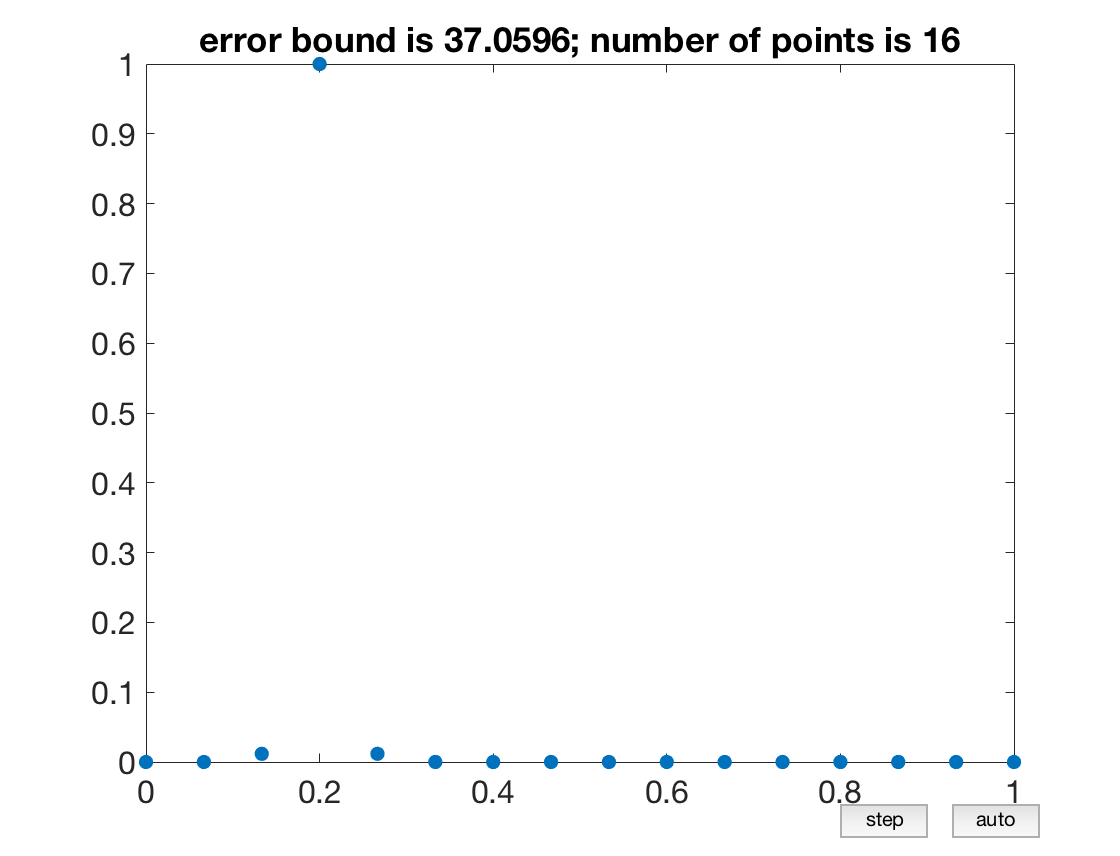
\includegraphics [width=4in]{localgui1.png}

\end{par} \vspace{1em}
\begin{par}
Step 2: add points to the peaky part
\end{par} \vspace{1em}
\begin{par}

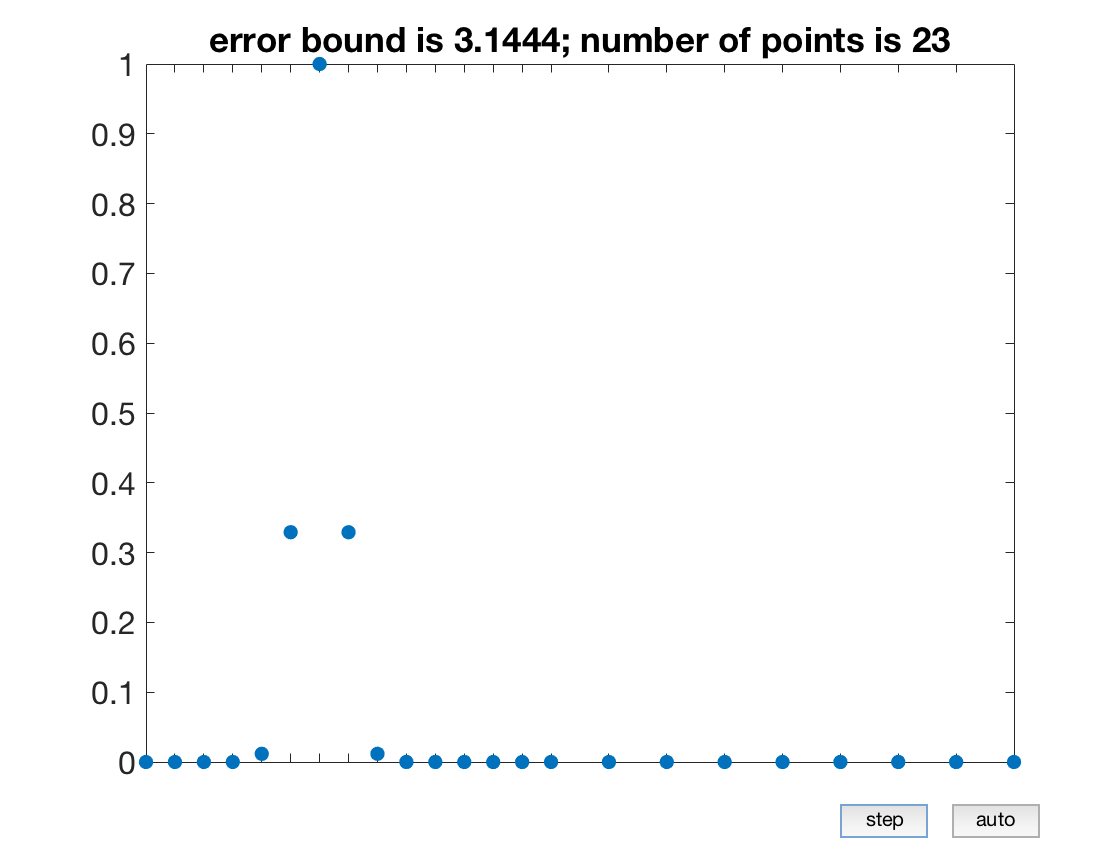
\includegraphics [width=4in]{localgui2.png}

\end{par} \vspace{1em}
\begin{par}
Step 6: after serveral iterations
\end{par} \vspace{1em}
\begin{par}

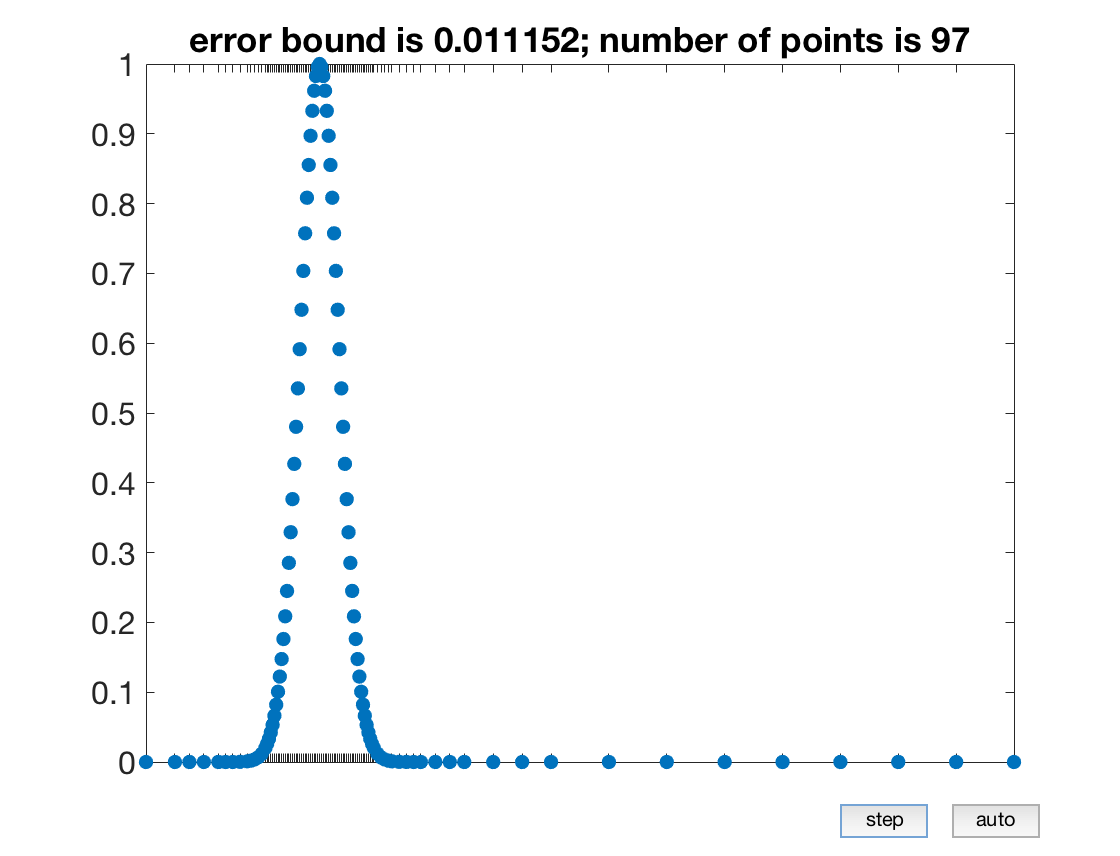
\includegraphics [width=4in]{localgui6.png}

\end{par} \vspace{1em}
\begin{par}
Step 7: reach the error tolerance
\end{par} \vspace{1em}
\begin{par}

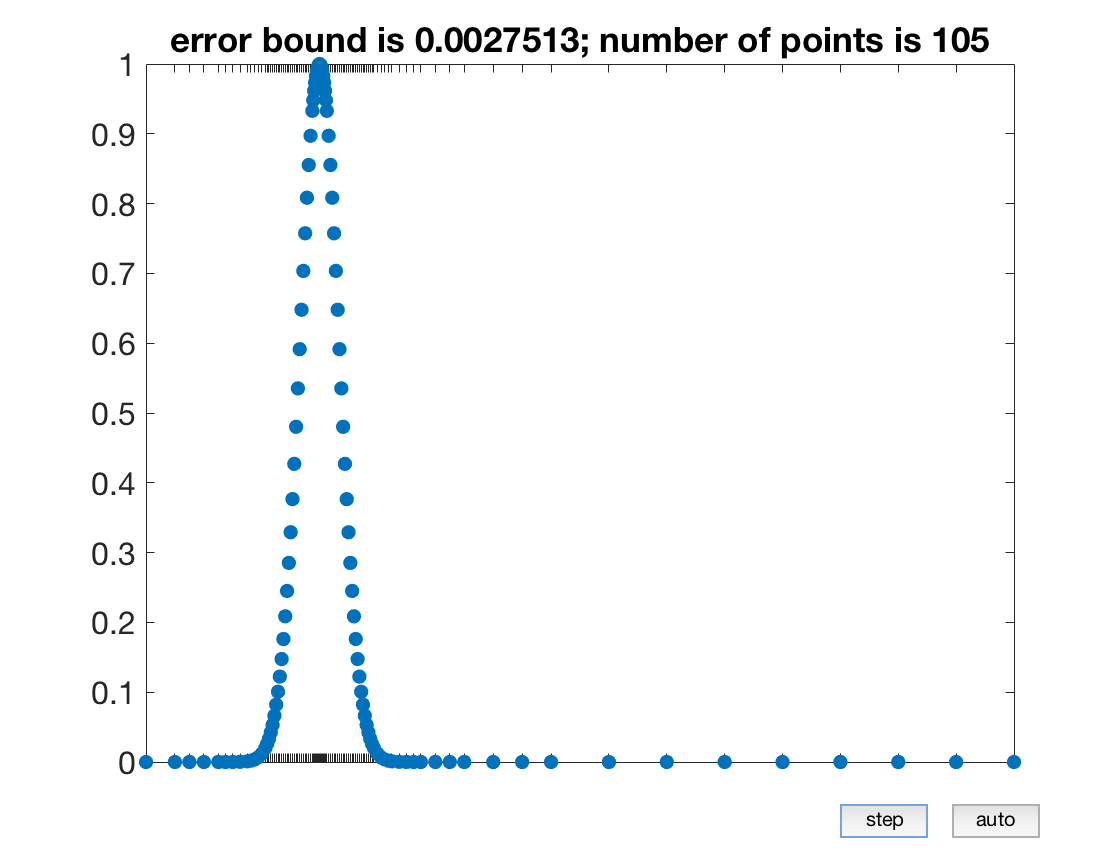
\includegraphics [width=4in]{localgui7.png}

\end{par} \vspace{1em}
\begin{par}
This process can also be reproduced by the following command: funappx\_g\_gui(@(x) exp(-1000*(x-0.2).\^{}2),0,1,1e-2,15,15);
\end{par} \vspace{1em}


\subsection*{References}

\begin{par}
[1] Sou-Cheng T. Choi, Yuhan Ding, Fred J.Hickernell, Xin Tong, "Local     Adaption for Approximation and Minimization of Univariate Functions,"     \textit{Journal of Complexity} 40, pp. 17-33, 2017.
\end{par} \vspace{1em}
\begin{par}
[2] Sou-Cheng T. Choi, Yuhan Ding, Fred J. Hickernell, Lan Jiang,     Lluis Antoni Jimenez Rugama, Xin Tong, Yizhi Zhang and Xuan Zhou,     GAIL: Guaranteed Automatic Integration Library (Version 2.2) [MATLAB     Software], 2017. Available from \begin{verbatim}GitHub\end{verbatim}.
\end{par} \vspace{1em}


\subsection*{Demos for funmin\_g}

\begin{par}

\end{par} \vspace{1em}
\begin{par}
\begin{verbatim}html\end{verbatim} \begin{verbatim}href="demo_funmin_g2.html">Comparing funmin_g with fminbnd</a\end{verbatim} \begin{verbatim}/html\end{verbatim}\%\% Find the minimum of a highly oscillating curve using \textbf{funmin\_g}
\end{par} \vspace{1em}


\subsection*{Function definition}

\begin{par}
Define a highly oscillating function as follows:
\end{par} \vspace{1em}
\begin{par}
\ensuremath{\backslash}[ f(x) = \ensuremath{\backslash}sin (10 \ensuremath{\backslash}pi x\^{}4 ) - x \ensuremath{\backslash}]
\end{par} \vspace{1em}
\begin{verbatim}
close all; clearvars; format compact; format short;
f = @(x) sin(10*pi*x.^4)-x;
\end{verbatim}


\subsection*{Function minimization}

\begin{par}
We use \textbf{funmin\_g} to approximate \ensuremath{\backslash}(f\ensuremath{\backslash}) over the interval \ensuremath{\backslash}([a,b]\ensuremath{\backslash}), where \ensuremath{\backslash}(a = 0\ensuremath{\backslash}) and \ensuremath{\backslash}(b = 2\ensuremath{\backslash}) with default parameter values:
\end{par} \vspace{1em}
\begin{verbatim}
a = 0; b = 2;
[fmin,outmin] = funmin_g(f, a, b);
\end{verbatim}


\subsection*{Plots of the function and its minimum}

\begin{par}
We plot \ensuremath{\backslash}(f(x)\ensuremath{\backslash}) and the approximate minimum returned by \textbf{funmin\_g} below. It is obvious that the approximation is not satisfactory. We compute the error by comparing to the true minimum returned by the Mathematica command, \texttt{N[Minimize[\{Sin[10 Pi x\^{}4] - x, 0 \ensuremath{<}= x \ensuremath{<}= 2\}, \{x\}],15]}.  The reason is probably that this function is not contained in the cone of functions sufficient for successful function minimization.
\end{par} \vspace{1em}
\begin{verbatim}
funmin_g_demo(fmin,outmin)
truefmin=-2.99843616266006;
truexmin=1.99843665971919;
max_abs_error = max(abs(truefmin-fmin))
\end{verbatim}

        \color{lightgray} \begin{verbatim}max_abs_error =
    0.0728
\end{verbatim} \color{black}
    
\includegraphics [width=4in]{gail_ug2_2_06.eps}


\subsection*{A fix}

\begin{par}
We can widen the cone by increasing the number of initial points given to \textbf{funmin\_g}.
\end{par} \vspace{1em}
\begin{verbatim}
inparam.a = a;
inparam.b = b;
inparam.ninit = 1000;
inparam.nmax = inparam.ninit*10;
[fmin2,outmin2] = funmin_g(f, inparam);

funmin_g_demo(fmin2,outmin2)

max_abs_error = max(abs(truefmin-fmin2))
\end{verbatim}

        \color{lightgray} \begin{verbatim}max_abs_error =
   9.3413e-09
\end{verbatim} \color{black}
    
\includegraphics [width=4in]{gail_ug2_2_07.eps}


\subsection*{References}

\begin{par}
[1] Sou-Cheng T. Choi, Yuhan Ding, Fred J.Hickernell, Xin Tong, "Local     Adaption for Approximation and Minimization of Univariate Functions,"   \textit{Journal of Complexity} 40, pp. 17-33, 2017.
\end{par} \vspace{1em}
\begin{par}
[2] Sou-Cheng T. Choi, Yuhan Ding, Fred J. Hickernell, Lan Jiang,     Lluis Antoni Jimenez Rugama, Xin Tong, Yizhi Zhang and Xuan Zhou,     GAIL: Guaranteed Automatic Integration Library (Version 2.2) [MATLAB     Software], 2017. Available from \begin{verbatim}GitHub\end{verbatim}.
\end{par} \vspace{1em}


\subsection*{Compare \textbf{funmin\_g} with \textbf{fminbnd}}

\begin{par}
Author: Xin Tong, July 2017
\end{par} \vspace{1em}


\subsection*{Function definition}

\begin{par}
Define a function with two minima as follows:
\end{par} \vspace{1em}
\begin{par}
\ensuremath{\backslash}[ f(x) = -5 \ensuremath{\backslash}exp(-100(x-0.2)\^{}2) - \ensuremath{\backslash}exp(-100(x-1)\^{}2). \ensuremath{\backslash}]
\end{par} \vspace{1em}
\begin{verbatim}
close all; clearvars; format compact; format short;
f = @(x) -5*exp((-100*(x-0.2).^2))-exp((-100.*(x-1).^2));
\end{verbatim}


\subsection*{Function minimization}

\begin{par}
We use \textbf{funmin\_g} to find the minimum of \ensuremath{\backslash}(f\ensuremath{\backslash}) over the interval \ensuremath{\backslash}([a,b]\ensuremath{\backslash}), where \ensuremath{\backslash}(a = 0\ensuremath{\backslash}) and \ensuremath{\backslash}(b = 1.5\ensuremath{\backslash}):
\end{par} \vspace{1em}
\begin{verbatim}
a = 0;
b = 1.5;
[fmin,out ] = funmin_g(f,a,b);
[xval,fval] = fminbnd(f,a,b);
\end{verbatim}


\subsection*{Plot of the function and minima}

\begin{par}
We plot \ensuremath{\backslash}(f(x)\ensuremath{\backslash}) and the global minimum value  returned by \textbf{funmin\_g} and and a local minimum by \textbf{fminbnd} below:
\end{par} \vspace{1em}
\begin{verbatim}
figure;
x = a:1e-6:b;
fminvec = fmin.*ones(size(x));
plot(x,f(x),'r-',out.intervals,[fmin,fmin],'go',xval,fval,'b*');
ylim([-6 1])
xlabel('$x$','interpreter','latex')
h_legend=legend('$f(x)$','funmin\_g','fminbnd');
set(h_legend,'interpreter','latex');
\end{verbatim}

\includegraphics [width=4in]{gail_ug2_2_08.eps}


\subsection*{References}

\begin{par}
[1] Sou-Cheng T. Choi, Yuhan Ding, Fred J.Hickernell, Xin Tong, "Local     Adaption for Approximation and Minimization of Univariate Functions,"     \textit{Journal of Complexity} 40, pp. 17-33, 2017.
\end{par} \vspace{1em}
\begin{par}
[2] Sou-Cheng T. Choi, Yuhan Ding, Fred J. Hickernell, Lan Jiang,     Lluis Antoni Jimenez Rugama, Xin Tong, Yizhi Zhang and Xuan Zhou,     GAIL: Guaranteed Automatic Integration Library (Version 2.2) [MATLAB     Software], 2017. Available from \begin{verbatim}GitHub\end{verbatim}.
\end{par} \vspace{1em}


\subsection*{Demos for integral\_g}

\begin{par}

\end{par} \vspace{1em}


\subsection*{Integrate a spiky function using \textbf{integral\_g}}

\begin{par}
Authors:  Fred Hickernell and Sou-Cheng Choi, August 2017
\end{par} \vspace{1em}


\subsection*{Function definition}

\begin{par}
This example is taken from [1], where a function is defined on \ensuremath{\backslash}( [0,1] \ensuremath{\backslash}) with twelve spikes.
\end{par} \vspace{1em}
\begin{verbatim}
close all; clear all; format compact; format short e;
[~,~,MATLABVERSION] = GAILstart(false);

xquad = 0.13579; %number used by quad to split interval into three parts
xleft = [0 xquad/2 xquad 3*xquad/2 2*xquad];
xctr = [2*xquad 1/4+xquad 1/2 3/4-xquad 1-2*xquad];
xrght = [1-2*xquad 1-3*xquad/2 1-xquad 1-xquad/2 1];
xall = [xleft xctr(2:5) xrght(2:5)]';
nnode = length(xall);

fbump = @(x) 4^3*((x.*(1-x)).^3).*((x>=0)&(x<=1)); %one bump
xplot = (0:0.002:1)'; %points to plot
spikyfun = @(x) foolfunmaker(x, @(x,c) fbump((x-c(1))/c(2)),...
    ones(nnode-1,1), [xall(1:nnode-1) diff(xall)]);
\end{verbatim}


\subsection*{Plot of the spiky function}

\begin{par}
In the following, we plot \ensuremath{\backslash}(f(x)\ensuremath{\backslash}) and show the data sampling points picked by MATLAB's built-in integration function \textbf{quad}, which explains why \textbf{quad} essentially gives the answer zero for our spiky function:
\end{par} \vspace{1em}
\begin{verbatim}
figure;
h = plot(xplot,spikyfun(xplot), 'k-', xall, zeros(nnode,1), 'k.');
axis([0 1 -0.3 1.1])
set(gca,'Ytick',-0.2:0.2:1)
legend(h,{'$f$','data'},'location','southeast')
\end{verbatim}

\includegraphics [width=4in]{gail_ug2_2_09.eps}


\subsection*{Integral approximation}

\begin{par}
We use MATLAB built-in functions and \textbf{integral\_g} [2] from GAIL [3] to integrate \ensuremath{\backslash}(f\ensuremath{\backslash}) over the unit interval:
\end{par} \vspace{1em}
\begin{verbatim}
a = 0;
b = 1;
abstol = 1e-11;
if MATLABVERSION >= 8,
    MATintegralspiky = integral(spikyfun,a,b,'AbsTol',abstol)
end
MATquadspiky = quad(spikyfun,a,b,abstol)
MATgailspiky = integral_g(spikyfun,a,b,abstol)
\end{verbatim}

        \color{lightgray} \begin{verbatim}MATintegralspiky =
   4.5714e-01
MATquadspiky =
   2.7021e-44
MATgailspiky =
   4.5714e-01
\end{verbatim} \color{black}
    

\subsection*{Compute apprroximation errors}

\begin{par}
The true integral value of the spiky function is \ensuremath{\backslash}(16/35\ensuremath{\backslash}). The following code computes absolute errors from the above approximation methods. Only \textbf{integral\_g} achieves the required accuracy with respect to the absolute tolerance of \ensuremath{\backslash}( 10\^{}\{-11\} \ensuremath{\backslash}) in this example.
\end{par} \vspace{1em}
\begin{verbatim}
integralspiky = 16/35;
if MATLABVERSION >= 8,
  abs_errors = abs(integralspiky - [MATintegralspiky, MATquadspiky, MATgailspiky])
else
  abs_errors = abs(integralspiky - [MATquadspiky, MATgailspiky])
end
if_meet_abstol = (abs_errors < abstol)
\end{verbatim}

        \color{lightgray} \begin{verbatim}abs_errors =
   6.1854e-10   4.5714e-01   1.4322e-14
if_meet_abstol =
     0     0     1
\end{verbatim} \color{black}
    

\subsection*{References}

\begin{par}
[1] Nick Clancy, Yuhan Ding, Caleb Hamilton, Fred J. Hickernell, and     Yizhi Zhang, "The Cost of Deterministic, Adaptive, Automatic     Algorithms: Cones, Not Balls," Journal of Complexity 30, pp. 21-45,     2014.
\end{par} \vspace{1em}
\begin{par}
[2] Fred J. Hickernell, Martha Razo, and Sunny Yun, "Reliable Adaptive     Numerical Integration", 2015+, working.
\end{par} \vspace{1em}
\begin{par}
[3] Sou-Cheng T. Choi, Yuhan Ding, Fred J. Hickernell, Lan Jiang,     Lluis Antoni Jimenez Rugama, Xin Tong, Yizhi Zhang and Xuan Zhou,     GAIL: Guaranteed Automatic Integration Library (Version 2.2) [MATLAB     Software], 2017. Available from \begin{verbatim}GitHub\end{verbatim}.
\end{par} \vspace{1em}


\subsection*{Demos for meanMC\_g}

\begin{par}
\begin{verbatim}html\end{verbatim} \begin{verbatim}href="count_success.html">Demo for meanMC_g</a\end{verbatim} \begin{verbatim}/html\end{verbatim}\%\% Counting the success rate of meanMC\_g  Authors: Lan Jiang and Sou-Cheng Choi, July 2017
\end{par} \vspace{1em}
\begin{par}
Define an integration problem as follows:
\end{par} \vspace{1em}
\begin{par}
\ensuremath{\backslash}[ I = \ensuremath{\backslash}int\_0\^{}1 x\^{}2 dx. \ensuremath{\backslash}]
\end{par} \vspace{1em}
\begin{par}
The analytical solution is 1/3. If we use \textbf{meanMC\_g} to estimate the integral with 1000 replications, we expect the success rate to be bigger than or equal to 1-\ensuremath{|}alpha\ensuremath{|}.
\end{par} \vspace{1em}
\begin{verbatim}
success = 0;
n = 1000;
in_param.reltol = 0; in_param.abstol = 1e-3;
in_param.alpha = 0.05; Yrand = @(n) rand(n,1).^2;
exactsol = 1/3;
for i = 1:n,
    tmu = meanMC_g(Yrand,in_param);
    check = abs(exactsol-tmu) < 1e-3;
    if check == 1,
        success = success + 1;
    end
end
disp(['Over ' num2str(n) ' replications, there are ' num2str(success) ' successes.'])
disp(['The success rate is ' num2str(success/n) ', which is larger than '...
    num2str(1-in_param.alpha) '.'])
\end{verbatim}

        \color{lightgray} \begin{verbatim}Over 1000 replications, there are 996 successes.
The success rate is 0.996, which is larger than 0.95.
\end{verbatim} \color{black}
    

\subsection*{Demos for cubMC\_g}

\begin{par}
\begin{verbatim}html\end{verbatim} \begin{verbatim}href="demo_normal_probabilities_cubMC.html">Computing normal probabilities</a\end{verbatim} \begin{verbatim}/html\end{verbatim}\%\% Estimation of normal probabilities by \textbf{cubMC\_g} Author: Lan Jiang, July 2017
\end{par} \vspace{1em}
\begin{par}
For $\bf{X}\sim N(\bf{\mu},\Sigma)$ , we will estimate the following probability:
\end{par} \vspace{1em}
\begin{par}
$$ P\left(\bf{a} \leq \bf{X} \leq \bf{b} \right) = \int_{\bf{a}}^{\bf{b}}
\frac{{\rm e}^{(\bf{x}-\bf{\mu})^t {\Sigma}^{-1}(\bf{x}-\bf{\mu})}}
{(2\pi)^{d/2}\left|{\Sigma}\right|^{1/2}}\,{\rm d}\bf{x}.$$
\end{par} \vspace{1em}
\begin{par}
We will approximate this probability using \textbf{cubMC\_g} and \textbf{meanMC\_g} GAIL methods. These are IID Monte Carlo algorithms. In order to facilitate the computations when $d$ is high (\ensuremath{\tilde{\;}}1000), we are going to apply a special transformation of the integrand proposed by Alan Genz.
\end{par} \vspace{1em}
\begin{verbatim}
function demo_normal_probabilities_cubMC
\end{verbatim}


\subsection*{Basic integration parameters set up}

\begin{par}
For all the examples, the dimension of the problem will be $d=30$. The user input tolerances are also set up below. \textit{abstol} is the absolute error tolerance, and \textit{reltol} the relative error tolerance. When \textit{reltol} is set to 0, the algorithms use pure absolute error bound, and viceversa. Finally, for simplicity we define the mean of the distribution to be $\bf{\mu}=\bf{0}$:
\end{par} \vspace{1em}
\begin{verbatim}
d = 3; % Dimension of the problem
abstol = 1e-2; % User input, absolute error bound
reltol = 0;  % User input, relative error bound
mu = zeros(d,1); % Mean of the distribution
\end{verbatim}


\subsection*{First test: $\Sigma=I_d$ (Monte Carlo cubMC\_g)}

\begin{par}
For this first example, we consider $\Sigma=I_d$, and $\bf{b}=-\bf{a}=(3.5,\dots,3.5)$. In this case, the solution of the integral is known so we can verify that the error conditions are met:
\end{par} \vspace{1em}
\begin{verbatim}
Sigma = eye(d); % We set the covariance matrix to the identity
factor = 3.5; hyperbox = [-factor*ones(1,d) ; factor*ones(1,d)]; % We define the integration limits
exactsol = (gail.stdnormcdf(factor)-gail.stdnormcdf(-factor))^d; % Exact solution of the integral

% Solution approx_prob and integration output parameters in out_param
[approx_prob,out_param] = multi_normcdf(hyperbox,mu,Sigma,abstol,reltol);
disp('Test 1: cubMC_g')
disp(['Estimated probability with cubMC_g is: ' num2str(approx_prob)])
disp(['The algorithm took ' num2str(out_param.time) ' seconds and '...
    num2str(out_param.ntot) ' points.'])
disp(['Real error was ' ...
    num2str(abs(exactsol-approx_prob))...
    ' which is less than the user input tolerance '...
    num2str(gail.tolfun(abstol,reltol,1,exactsol,'max')) '.'])
\end{verbatim}


\subsection*{Second test: $\Sigma=0.4I_d + 0.6\bf{1}\bf{1}^T$ (Monte Carlo cubMC\_g)}

\begin{par}
For this second example, we consider $\Sigma=0.4I_d + 0.6\bf{1}\bf{1}^T$ ($1$ on the diagonal, $0.6$ off the diagional), $\bf{a}=(-\infty,\dots,-\infty)$, and $\bf{b}=\sqrt{d}(U_1,\dots,U_d)$ ($\bf{b}$ is chosen randomly). The solution for this integral is known too so we can verify the real error:
\end{par} \vspace{1em}
\begin{verbatim}
sig = 0.6; Sigma = sig*ones(d,d); Sigma(1:d+1:d*d) = 1; % We set the covariance matrix
hyperbox = [-Inf*ones(1,d) ; sqrt(d)*rand(1,d)]; % We define the integration limits
[exactsol , ~] = cubMC_g(...
  @(t) prod(gail.stdnormcdf(bsxfun(@plus,hyperbox(2,:),...
  sqrt(sig)*t)/sqrt(1-sig)),2),...
  [-Inf;Inf],'normal',abstol,0);  % Exact solution of the integral

% Solution approx_prob and integration output parameters in out_param
[approx_prob,out_param] = multi_normcdf(hyperbox,mu,Sigma,abstol,reltol);
disp('Test 2: cubMC_g')
disp(['Estimated probability with cubMC_g is: ' num2str(approx_prob)])
disp(['The algorithm took ' num2str(out_param.time) ' seconds and '...
    num2str(out_param.ntot) ' points.'])
disp(['Real error was ' ...
    num2str(abs(exactsol-approx_prob))...
    ' which is less than the user input tolerance '...
    num2str(gail.tolfun(abstol,reltol,1,exactsol,'max')) '.'])
\end{verbatim}


\subsection*{Third test: $\Sigma=0.4I_d + 0.6\bf{1}\bf{1}^T$ (Monte Carlo cubMC\_g)}

\begin{par}
For this last example, we consider the same covariance matrix as before but $\bf{a}=-d/3(U_1,\dots,U_d)$, and $\bf{b}=d/3(U_{d+1},\dots,U_{2d})$ (both $\bf{a}$ and $\bf{b}$ are chosen randomly):
\end{par} \vspace{1em}
\begin{verbatim}
hyperbox = [-(d/3)*rand(1,d) ; (d/3)*rand(1,d)]; % We define the integration limits

% Solution approx_prob and integration output parameters in out_param
[approx_prob,out_param] = multi_normcdf(hyperbox,mu,Sigma,abstol,reltol);
disp('Test 3: cubMC_g')
disp(['Estimated probability with cubMC_g is: ' num2str(approx_prob)])
disp(['The algorithm took ' num2str(out_param.time) ' seconds and '...
    num2str(out_param.n) ' points.'])
\end{verbatim}


\subsection*{APPENDIX: Auxiliary function definitions}

\begin{par}
These two functions are defined for all the above test examples. \textit{multi\_normcdf} is a redefinition of cubMC\_g prepared to computed normal probabilites based on Alan Genz's transformation. \textit{f} is the function resulting from applying Alan Genz's transform that that will be called in either cubMC\_g or meanMC\_g.
\end{par} \vspace{1em}
\begin{verbatim}
function [Q,param] = multi_normcdf(hyperbox,mu,Sigma,abstol,reltol)
% multi_normcdf computes the cumulative distribution function of the
% multivariate normal distribution with mean mu, covariance matrix Sigma
% and within the region defined by hyperbox.
    hyperbox = bsxfun(@minus, hyperbox,mu');
    C = chol(Sigma)'; d = size(C,1);
    a = hyperbox(1,1)/C(1,1); b = hyperbox(2,1)/C(1,1);
    s = gail.stdnormcdf(a); e = gail.stdnormcdf(b);
    [Q,param] = cubMC_g(...
        @(x) f(s,e,hyperbox,x,C), [zeros(1,d-1);ones(1,d-1)],...
        'uniform',abstol,reltol);
end

function f_eval = f(s,e,hyperbox,w,C)
% This is the integrand resulting from applying Alan Genz's transformation,
% which is recursively defined.
    f_eval = (e-s)*ones(size(w,1),1);
    aux = ones(size(w,1),1);
    y = [];
    for i = 2:size(hyperbox,2);
        y = [y gail.stdnorminv(s+w(:,i-1).*(e-s))];
        aux = sum(bsxfun(@times,C(i,1:i-1),y),2);
        a = (hyperbox(1,i)-aux)/C(i,i);
        b = (hyperbox(2,i)-aux)/C(i,i);
        s = gail.stdnormcdf(a);
        e = gail.stdnormcdf(b);
        f_eval = f_eval .* (e-s);
    end
end
\end{verbatim}
\begin{verbatim}
end
\end{verbatim}


\subsection*{References}

\begin{par}
[1] Fred J. Hickernell, Lluis Antoni Jimenez Rugama "Reliable adaptive     cubature using digital sequences", Monte Carlo and Quasi-Monte Carlo     Methods: MCQMC, Leuven, Belgium, April 2014 (R. Cools and D. Nuyens,     eds.), Springer Proceedings in Mathematics and Statistics, vol. 163,     Springer-Verlag, Berlin, 2016, arXiv:1410.8615 [math.NA], pp.     367-383.
\end{par} \vspace{1em}
\begin{par}
[2] Fred J. Hickernell, Lan Jiang, Yuewei Liu, and Art B. Owen,     "Guaranteed conservative fixed width confidence intervals via Monte     Carlo sampling," Monte Carlo and Quasi-Monte Carlo Methods 2012     (J. Dick, F. Y. Kuo, G. W. Peters, and I. H. Sloan, eds.),     Springer-Verlag, Berlin, pp. 105-128, 2014.
\end{par} \vspace{1em}
\begin{par}
[3] Sou-Cheng T. Choi, Yuhan Ding, Fred J. Hickernell, Lan Jiang,     Lluis Antoni Jimenez Rugama, Xin Tong, Yizhi Zhang and Xuan Zhou,     GAIL: Guaranteed Automatic Integration Library (Version 2.2) [MATLAB     Software], 2017. Available from \begin{verbatim}GitHub\end{verbatim}.\%\% Demos for cubSobol\_g
\end{par} \vspace{1em}
\begin{par}

\end{par} \vspace{1em}


\subsection*{Estimation of normal probabilities by \textbf{cubSobol\_g}}

\begin{par}
Author: Lluis Antoni Jimenez Rugama, July 2017
\end{par} \vspace{1em}
\begin{par}
For $\bf{X}\sim N(\bf{\mu},\Sigma)$ , we will estimate the following probability:
\end{par} \vspace{1em}
\begin{par}
$$ P\left(\bf{a} \leq \bf{X} \leq \bf{b} \right) = \int_{\bf{a}}^{\bf{b}}
\frac{{\rm e}^{(\bf{x}-\bf{\mu})^t {\Sigma}^{-1}(\bf{x}-\bf{\mu})}}
{(2\pi)^{d/2}\left|{\Sigma}\right|^{1/2}}\,{\rm d}\bf{x}.$$
\end{par} \vspace{1em}
\begin{par}
We will approximate this probability using \textbf{cubSobol\_g} and \textbf{meanMC\_g} GAIL methods. These are quasi-Monte Carlo and IID Monte Carlo algorithms. In order to facilitate the computations when $d$ is high (\ensuremath{\tilde{\;}}1000), we are going to apply a special transformation of the integrand proposed by Alan Genz.
\end{par} \vspace{1em}
\begin{verbatim}
function demo_normal_probabilities
\end{verbatim}


\subsection*{Basic integration parameters set up}

\begin{par}
For all the examples, the dimension of the problem will be $d=30$. The user input tolerances are also set up below. \textit{abstol} is the absolute error tolerance, and \textit{reltol} the relative error tolerance. When \textit{reltol} is set to 0, the algorithms use pure absolute error bound, and viceversa. Finally, for simplicity we define the mean of the distribution to be $\bf{\mu}=\bf{0}$:
\end{par} \vspace{1em}
\begin{verbatim}
d = 30; % Dimension of the problem
abstol = 1e-3; % User input, absolute error bound
reltol = 0;  % User input, relative error bound
mu = zeros(d,1); % Mean of the distribution
\end{verbatim}


\subsection*{First test: $\Sigma=I_d$ (quasi-Monte Carlo cubSobol\_g)}

\begin{par}
For this first example, we consider $\Sigma=I_d$, and $\bf{b}=-\bf{a}=(3.5,\dots,3.5)$. In this case, the solution of the integral is known so we can verify that the error conditions are met:
\end{par} \vspace{1em}
\begin{verbatim}
Sigma = eye(d); % We set the covariance matrix to the identity
factor = 3.5; hyperbox = [-factor*ones(1,d) ; factor*ones(1,d)]; % We define the integration limits
exactsol = (gail.stdnormcdf(factor)-gail.stdnormcdf(-factor))^d; % Exact solution of the integral

% Solution approx_prob and integration output parameters in out_param
[approx_prob,out_param] = multi_normcdf(hyperbox,mu,Sigma,abstol,reltol);
disp('Test 1: cubSobol_g')
disp(['Estimated probability with cubSobol_g is: ' num2str(approx_prob)])
disp(['The algorithm took ' num2str(out_param.time) ' seconds and '...
    num2str(out_param.n) ' points.'])
disp(['Real error was ' ...
    num2str(abs(exactsol-approx_prob))...
    ' which is less than the user input tolerance '...
    num2str(gail.tolfun(abstol,reltol,1,exactsol,'max')) '.'])
\end{verbatim}


\subsection*{Second test: $\Sigma=0.4I_d + 0.6\bf{1}\bf{1}^T$ (quasi-Monte Carlo cubSobol\_g)}

\begin{par}
For this second example, we consider $\Sigma=0.4I_d + 0.6\bf{1}\bf{1}^T$ ($1$ on the diagonal, $0.6$ off the diagional), $\bf{a}=(-\infty,\dots,-\infty)$, and $\bf{b}=\sqrt{d}(U_1,\dots,U_d)$ ($\bf{b}$ is chosen randomly). The solution for this integral is known too so we can verify the real error:
\end{par} \vspace{1em}
\begin{verbatim}
sig = 0.6; Sigma = sig*ones(d,d); Sigma(1:d+1:d*d) = 1; % We set the covariance matrix
hyperbox = [-Inf*ones(1,d) ; sqrt(d)*rand(1,d)]; % We define the integration limits
[exactsol , ~] = cubSobol_g(...
  @(t) prod(gail.stdnormcdf(bsxfun(@plus,hyperbox(2,:),...
  sqrt(sig)*t)/sqrt(1-sig)),2),...
  [-Inf;Inf],'normal',abstol/10^3,0);  % Exact solution of the integral

% Solution approx_prob and integration output parameters in out_param
[approx_prob,out_param] = multi_normcdf(hyperbox,mu,Sigma,abstol,reltol);
disp('Test 2: cubSobol_g')
disp(['Estimated probability with cubSobol_g is: ' num2str(approx_prob)])
disp(['The algorithm took ' num2str(out_param.time) ' seconds and '...
    num2str(out_param.n) ' points.'])
disp(['Real error was ' ...
    num2str(abs(exactsol-approx_prob))...
    ' which is less than the user input tolerance '...
    num2str(gail.tolfun(abstol,reltol,1,exactsol,'max')) '.'])
\end{verbatim}


\subsection*{Third test: $\Sigma=0.4I_d + 0.6\bf{1}\bf{1}^T$ (quasi-Monte Carlo cubSobol\_g)}

\begin{par}
For this last example, we consider the same covariance matrix as before but $\bf{a}=-d/3(U_1,\dots,U_d)$, and $\bf{b}=d/3(U_{d+1},\dots,U_{2d})$ (both $\bf{a}$ and $\bf{b}$ are chosen randomly):
\end{par} \vspace{1em}
\begin{verbatim}
hyperbox = [-(d/3)*rand(1,d) ; (d/3)*rand(1,d)]; % We define the integration limits

% Solution approx_prob and integration output parameters in out_param
[approx_prob,out_param] = multi_normcdf(hyperbox,mu,Sigma,abstol,reltol);
disp('Test 3: cubSobol_g')
disp(['Estimated probability with cubSobol_g is: ' num2str(approx_prob)])
disp(['The algorithm took ' num2str(out_param.time) ' seconds and '...
    num2str(out_param.n) ' points.'])
\end{verbatim}


\subsection*{Third test with IID Monte Carlo (Monte Carlo meanMC\_g)}

\begin{par}
We repeat the third test but we use the IID Monte Carlo algorithm instead:
\end{par} \vspace{1em}
\begin{verbatim}
C = chol(Sigma)'; % Alan Genz's transform parameters
a = hyperbox(1,1)/C(1,1); b = hyperbox(2,1)/C(1,1); % Alan Genz's transform parameters
s = gail.stdnormcdf(a); e = gail.stdnormcdf(b); % Alan Genz's transform parameters

% Solution approx_prob and integration output parameters in out_param
[approx_prob,out_param] = meanMC_g(@(n) f(s,e,hyperbox,rand(n,d-1),C),...
    abstol,reltol,'tbudget',5000);
disp('Test 3: meanMC_g')
disp(['Estimated probability with meanMC_g is: ' num2str(approx_prob)])
disp(['The algorithm took ' num2str(out_param.time) ' seconds and '...
    num2str(out_param.n) ' points.'])
\end{verbatim}


\subsection*{APPENDIX: Auxiliary function definitions}

\begin{par}
These two functions are defined for all the above test examples. \textit{multi\_normcdf} is a redefinition of cubSobol\_g prepared to computed normal probabilites based on Alan Genz's transformation. \textit{f} is the function resulting from applying Alan Genz's transform that that will be called in either cubSobol\_g or meanMC\_g.
\end{par} \vspace{1em}
\begin{verbatim}
function [p,out, y, kappanumap] = multi_normcdf(hyperbox,mu,Sigma,...
        abstol,reltol)
% multi_normcdf computes the cumulative distribution function of the
% multivariate normal distribution with mean mu, covariance matrix Sigma
% and within the region defined by hyperbox.
    hyperbox = bsxfun(@minus, hyperbox,mu');
    C = chol(Sigma)'; d = size(C,1);
    a = hyperbox(1,1)/C(1,1); b = hyperbox(2,1)/C(1,1);
    s = gail.stdnormcdf(a); e = gail.stdnormcdf(b);
    [p, out, y, kappanumap] = cubSobol_g(...
        @(x) f(s,e,hyperbox,x,C), [zeros(1,d-1);ones(1,d-1)],...
        'uniform',abstol,reltol);
end

function f_eval = f(s,e,hyperbox,w,C)
% This is the integrand resulting from applying Alan Genz's transformation,
% which is recursively defined.
    f_eval = (e-s)*ones(size(w,1),1);
    aux = ones(size(w,1),1);
    y = [];
    for i = 2:size(hyperbox,2);
        y = [y gail.stdnorminv(s+w(:,i-1).*(e-s))];
        aux = sum(bsxfun(@times,C(i,1:i-1),y),2);
        a = (hyperbox(1,i)-aux)/C(i,i);
        b = (hyperbox(2,i)-aux)/C(i,i);
        s = gail.stdnormcdf(a);
        e = gail.stdnormcdf(b);
        f_eval = f_eval .* (e-s);
    end
end
\end{verbatim}
\begin{verbatim}
end
\end{verbatim}


\subsection*{References}

\begin{par}
[1] Fred J. Hickernell, Lluis Antoni Jimenez Rugama "Reliable adaptive     cubature using digital sequences", Monte Carlo and Quasi-Monte Carlo     Methods: MCQMC, Leuven, Belgium, April 2014 (R. Cools and D. Nuyens,     eds.), Springer Proceedings in Mathematics and Statistics, vol. 163,     Springer-Verlag, Berlin, 2016, arXiv:1410.8615 [math.NA], pp.     367-383.
\end{par} \vspace{1em}
\begin{par}
[2] Fred J. Hickernell, Lan Jiang, Yuewei Liu, and Art B. Owen,     "Guaranteed conservative fixed width confidence intervals via Monte     Carlo sampling," Monte Carlo and Quasi-Monte Carlo Methods 2012     (J. Dick, F. Y. Kuo, G. W. Peters, and I. H. Sloan, eds.),     Springer-Verlag, Berlin, pp. 105-128, 2014.
\end{par} \vspace{1em}
\begin{par}
[3] Sou-Cheng T. Choi, Yuhan Ding, Fred J. Hickernell, Lan Jiang,     Lluis Antoni Jimenez Rugama, Xin Tong, Yizhi Zhang and Xuan Zhou,     GAIL: Guaranteed Automatic Integration Library (Version 2.2) [MATLAB     Software], 2017. Available from \begin{verbatim}GitHub\end{verbatim}.\% TEST\_CUBSOBOL\_G This is the driver script to test cubSobol\_g algorithm
\end{par} \vspace{1em}
\begin{verbatim}
%using seven integrands of dimensions up to 8
%clear all;close all;clc;
function [ut_abserr,ut_relerr,abstol,reltol] = Test_cubSobol_g
%[
dimsize = 3;
indexsize = 2;
abstol = 1e-3;
reltol = abstol;
format long
in_param.measure  = 'uniform';
disp('');
disp(horzcat('Dim  ', ' FcnIdx ',  '      Q    ','         f_true     ',...
    '          Err      ','      Sample Used    ', '         Stats  '));
disp(        '-----------------------------------------------------------------------------------------------------');
ut_abserr = nan(dimsize,indexsize);
ut_relerr = nan(dimsize,indexsize);
for dim=1:dimsize
  in_param.dim =dim;%the function dimension
  startingpoint = zeros(1,in_param.dim);%the lower limits of the integral
  endingpoint = ones(1,in_param.dim);%the upper limits of the integral
  hyperbox = [startingpoint;endingpoint];% the integration interval
  in_param.abstol = abstol;% the absolute tolerance
  in_param.reltol = reltol;% the relative tolerance
  in_param.alpha = 1e-2;% the uncertainty
  in_param.nSig = 1e4;% the sample size to estimate sigma
  in_param.n1 = 1e4;% the initial sample size to estimate Q
  %in_param.fudge =1.2;% standard deviation inflation factor
  in_param.timebudget = 300;% time budget
  in_param.nbudget = 1e10;% sample budget
  alpha = ones(1,in_param.dim);
  beta = 1./ (1:in_param.dim);
  r=2; % three coefficients in genz_test_fun and genz_test_fun_true
  for index=1:indexsize % index refers to different integrands in genz_test_fun
    test_function = @(x)genz_test_fun(x,index,in_param.dim,alpha,beta,r);
    % the test function
    f_true = genz_test_fun_true (hyperbox,index,in_param.dim,alpha,beta,r);
    % true integral of the test function
    [Q,out_param]=cubSobol_g(test_function,hyperbox,in_param);
    % the results by using cubLattice_g
    abserr = abs(Q-f_true);% the absolute error
    relerr = abs((Q-f_true)/f_true);% the relative error
    numstr=horzcat(num2str(dim), '     ', num2str(index), '       ',...
        num2str(Q,'%10.5e'), '       ', num2str(f_true,'%10.5e'),...
        '       ', num2str(abserr,'%10.5e'),...
        '         ', num2str(out_param.n));
    % print the results
    if abserr > in_param.abstol && relerr > in_param.reltol,
    %if both absolute error and relative error does not meet tolerance
      disp([numstr,'            NoErrMet']);% mark it as "both err exceed"
    elseif abserr < in_param.abstol && relerr > in_param.reltol,
        % if only relative error does not meet the tolerance
        disp([numstr,'             AbsErrMet']);% mark it as "rel err exceed"
    elseif abserr > in_param.abstol && relerr < in_param.reltol,
        %if only the absolute error does not meet the tolerance
        disp([numstr,'            RelErrMet']);% mark it as "abs err exceed"
    else
        disp([numstr,'             BothErrMet']);% otherwise disp "OK"
    end
    ut_abserr(dim,index) = abserr;
    ut_relerr(dim,index) = relerr;
  end
end
end
\end{verbatim}


\subsection*{The following output was obtained on 2014-10-13  by Lan Jiang}

\begin{par}
Dim   FcnIdx       Q            f\_true             Error            Sample Used        status ---------------------------------------------------------------------------------------------- 1     1       8.41429e-01       8.41471e-01       4.16988e-05         975445             BothErrMet 1     2       7.85471e-01       7.85398e-01       7.25717e-05         1236277             BothErrMet 1     3       3.75266e-01       3.75000e-01       2.65681e-04         2129675             BothErrMet 1     4       7.46756e-01       7.46824e-01       6.76680e-05         1728700             BothErrMet 1     5       6.32161e-01       6.32121e-01       4.03169e-05         1462142             BothErrMet 1     6       1.71795e+00       1.71828e+00       3.29683e-04         2997628             BothErrMet 1     7       1.38083e+00       1.38039e+00       4.39163e-04         4339991             BothErrMet 2     1       4.96824e-01       4.96751e-01       7.24267e-05         3649273             BothErrMet 2     2       7.28163e-01       7.28296e-01       1.33307e-04         1179211             BothErrMet 2     3       1.01966e-01       1.01852e-01       1.14565e-04         707289     AbsErrMet 2     4       6.89122e-01       6.88992e-01       1.30139e-04         1604731             BothErrMet 2     5       4.97274e-01       4.97440e-01       1.65640e-04         1241193             BothErrMet Warning: At step 2, tried to evaluate at 27050414 samples, which is more than the remaining 16945370 samples. We will use all the sample left to estimate the mean. \ensuremath{>} In meanMC\_g\ensuremath{>}meanMC\_g\_err at 493   In meanMC\_g\ensuremath{>}meanmctolfun at 243   In meanMC\_g at 208   In cubMC\_g at 211   In Test\_cubMC\_g at 30 2     6       1.11489e+00       1.11469e+00       2.08576e-04         16965382             BothErrMet 2     7       1.80862e+00       1.80819e+00       4.32649e-04         10925304             BothErrMet 3     1       6.21012e-02       6.23593e-02       2.58075e-04         6206320     AbsErrMet 3     2       6.62509e-01       6.62570e-01       6.02562e-05         1193449             BothErrMet 3     3       2.17371e-02       2.17014e-02       3.57372e-05         160438     AbsErrMet 3     4       6.20919e-01       6.20903e-01       1.52024e-05         1596268             BothErrMet 3     5       3.82965e-01       3.83055e-01       8.95927e-05         1042167             BothErrMet Warning: At step 2, tried to evaluate at 27836133 samples, which is more than the remaining 18770218 samples. We will use all the sample left to estimate the mean. \ensuremath{>} In meanMC\_g\ensuremath{>}meanMC\_g\_err at 493   In meanMC\_g\ensuremath{>}meanmctolfun at 243   In meanMC\_g at 208   In cubMC\_g at 211   In Test\_cubMC\_g at 30 3     6       4.40912e-01       4.40984e-01       7.16979e-05         18790230             BothErrMet 3     7       2.16887e+00       2.16831e+00       5.59135e-04         28582950             BothErrMet 4     1       -3.52095e-01       -3.51764e-01       3.31374e-04         6517309             BothErrMet 4     2       5.88689e-01       5.88680e-01       9.02213e-06         1225452             BothErrMet 4     3       3.76752e-03       3.80556e-03       3.80333e-05         40451     AbsErrMet 4     4       5.43599e-01       5.43373e-01       2.25590e-04         1516358             BothErrMet 4     5       2.86912e-01       2.86844e-01       6.78729e-05         853151             BothErrMet 4     6       1.25321e-01       1.25251e-01       7.07149e-05         11047422             BothErrMet 4     7       2.16562e+00       2.16593e+00       3.11327e-04         93662781             BothErrMet 5     1       -6.49227e-01       -6.49331e-01       1.03821e-04         4553095             BothErrMet 5     2       5.13536e-01       5.13409e-01       1.27207e-04         1212257             BothErrMet 5     3       5.44026e-04       5.67130e-04       2.31041e-05         20012     AbsErrMet 5     4       4.64590e-01       4.64603e-01       1.29513e-05         1455926             BothErrMet 5     5       2.09824e-01       2.09952e-01       1.28909e-04         680797             BothErrMet 5     6       2.77841e-02       2.77308e-02       5.33210e-05         3955141     AbsErrMet Warning: At step 2, tried to evaluate at 363333179 samples, which is more than the remaining 156107201 samples. We will use all the sample left to estimate the mean. \ensuremath{>} In meanMC\_g\ensuremath{>}meanMC\_g\_err at 493   In meanMC\_g\ensuremath{>}meanmctolfun at 243   In meanMC\_g at 208   In cubMC\_g at 211   In Test\_cubMC\_g at 30 5     7       1.13488e+00       1.13532e+00       4.41697e-04         156127213             BothErrMet 6     1       -7.69317e-01       -7.69376e-01       5.96515e-05         2903377             BothErrMet 6     2       4.41269e-01       4.41474e-01       2.04762e-04         1134235             BothErrMet 6     3       8.33814e-05       7.34937e-05       9.88770e-06         20012     AbsErrMet 6     4       3.90190e-01       3.90227e-01       3.73760e-05         1342631             BothErrMet 6     5       1.51006e-01       1.50939e-01       6.71353e-05         508574             BothErrMet 6     6       5.35235e-03       5.02927e-03       3.23080e-04         998551     AbsErrMet Warning: At step 2, tried to evaluate at 369500174 samples, which is more than the remaining 138997141 samples. We will use all the sample left to estimate the mean. \ensuremath{>} In meanMC\_g\ensuremath{>}meanMC\_g\_err at 493   In meanMC\_g\ensuremath{>}meanmctolfun at 243   In meanMC\_g at 208   In cubMC\_g at 211   In Test\_cubMC\_g at 30 6     7       -2.32827e+00       -2.32730e+00       9.70403e-04         139017153             BothErrMet 7     1       -6.97541e-01       -6.97824e-01       2.82984e-04         4242250             BothErrMet 7     2       3.75388e-01       3.75484e-01       9.57243e-05         1067298             BothErrMet 7     3       8.01023e-06       8.42590e-06       4.15666e-07         20012     AbsErrMet 7     4       3.23245e-01       3.23235e-01       9.80560e-06         1195993             BothErrMet 7     5       1.06979e-01       1.06978e-01       1.26088e-06         359100             BothErrMet 7     6       8.80028e-04       7.72320e-04       1.07708e-04         434550     AbsErrMet 7     7       -1.10547e+01       -1.10568e+01       2.12771e-03         97127597     RelErrMet 8     1       -4.66861e-01       -4.67036e-01       1.74775e-04         7976409             BothErrMet 8     2       3.16567e-01       3.16602e-01       3.49663e-05         943146             BothErrMet 8     3       9.37483e-07       8.66209e-07       7.12746e-08         20012     AbsErrMet 8     4       2.64938e-01       2.64801e-01       1.37326e-04         1044264             BothErrMet 8     5       7.49463e-02       7.49531e-02       6.81415e-06         254752             BothErrMet 8     6       5.80123e-04       1.02833e-04       4.77290e-04         20012     AbsErrMet 8     7       -3.06063e+01       -3.06091e+01       2.80834e-03         41618674     RelErrMet
\end{par} \vspace{1em}
\begin{verbatim}
end
\end{verbatim}



\end{document}
    
